\documentclass[oneside,a4paper,spanish,links]{amca}

\usepackage{graphicx}
\usepackage{amsmath,amssymb,bm}
\usepackage{booktabs,array,longtable,tabularx}
\usepackage{fancyvrb}
\usepackage[section]{placeins}
\usepackage{xurl}
\usepackage{microtype}

\graphicspath{{../figures/}}
\setcounter{tocdepth}{2}
\setcounter{secnumdepth}{3}
\emergencystretch=2em
\renewcommand{\contentsname}{CONTENIDO}
\renewcommand{\listfigurename}{ÍNDICE DE FIGURAS}
\newcolumntype{Y}{>{\raggedright\arraybackslash}X}

\title{INFORME INTEGRAL DE RESULTADOS DEL MODELO ESTRUCTURAL,\\
ROTODINÁMICO Y SÍSMICO DE UN AEROGENERADOR}
\englishtitle{COMPREHENSIVE RESULTS REPORT FOR THE STRUCTURAL,\\
ROTORDYNAMIC AND SEISMIC MODEL OF A WIND TURBINE}
\author{Nicolás A. Useche Castillo}
\affil{Departamento de Ingeniería Mecánica, Universidad de los Andes, Bogotá D.C., Colombia,\\
n.useche@uniandes.edu.co}

\hypersetup{
  pdftitle={Informe integral de resultados del modelo estructural, rotodinámico y sísmico},
  pdfauthor={Nicolás A. Useche Castillo},
  colorlinks=true,
  linkcolor=blue,
  citecolor=blue,
  urlcolor=blue
}

\begin{document}
\vspace{3cm}
\maketitle

\begin{keywords}
turbina eólica, elementos finitos, viga de Timoshenko,
conversión de mallas, modos rígidos, frecuencias naturales, giroscopía, Campbell,
transformación multiblade, excitación sísmica, problema de autovalores.
\end{keywords}

\begin{abstract}
Este informe presenta e interpreta los resultados del modelo estructural,
rotodinámico y sísmico de un aerogenerador. Se describe la conversión de la malla
heredada, la formulación del elemento de viga de Timoshenko tridimensional, la
condensación por restricciones multipunto y la incorporación de masas rígidas. El
espectro del elemento libre aislado contiene exactamente seis modos de cuerpo rígido y
seis frecuencias naturales deformacionales; el ensamblaje global libre conserva seis
modos rígidos, mientras que la base fija elimina los modos nulos. Se interpretan además
el equilibrio con gravedad y centrifugación, la giroscopía, el amortiguamiento de
Rayleigh, la inserción de cargas aerodinámicas, la transformación multiblade, el problema
cuadrático de autovalores, el diagrama de Campbell y la respuesta sísmica integrada con
Newmark. Cada resultado se acompaña de su error relativo o criterio esperado. Los
parámetros de tren, amortiguamiento y excitación sísmica empleados son casos de
referencia numérica; no constituyen una predicción calibrada de una turbina comercial.

\vspace{6pt}
\noindent\textbf{Abstract.} This report presents and interprets the results of a
structural, rotordynamic and seismic wind-turbine model. It describes legacy-mesh
conversion, the three-dimensional Timoshenko beam formulation, exact multi-point
condensation and rigid-mass insertion. The isolated free element contains exactly six
rigid-body modes and six positive deformational natural frequencies; the complete free
assembly retains six global rigid-body modes, whereas the fixed-base model has no null
modes. The report also explains equilibrium under gravity and centrifugal loading,
gyroscopic coupling, Rayleigh damping, aerodynamic-load insertion, multiblade
transformation, the quadratic eigenvalue problem, Campbell tracking and Newmark seismic
integration. Every result is reported together with its relative error or expected
numerical target. Drivetrain, damping and earthquake inputs are numerical reference
cases rather than a calibrated commercial-turbine prediction.
\end{abstract}

\tableofcontents
\clearpage
\listoffigures
\clearpage

\section*{NOMENCLATURA Y CONVENCIONES}
\addcontentsline{toc}{section}{Nomenclatura y convenciones}
\begin{center}
\small
\begin{tabularx}{\textwidth}{@{}p{0.19\textwidth}Y@{}}
\toprule
\textbf{Símbolo} & \textbf{Definición} \\
\midrule
$\bm q$, $\dot{\bm q}$, $\ddot{\bm q}$ & desplazamiento, velocidad y aceleración generalizados \\
$\bm M$ & matriz de masa consistente \\
$\bm C_s$, $\bm C_a$, $\bm G$ & amortiguamiento estructural, amortiguamiento aerodinámico y matriz giroscópica \\
$\bm K_e$, $\bm K_g$, $\bm K_\Omega$, $\bm K_a$ & rigidez elástica, geométrica, centrífuga y tangente aerodinámica \\
$\bm T_c$, $\bm P$ & transformación de restricciones y transformación multiblade compuesta \\
$\bm R_{\mathrm{full}}$, $\bm\Gamma_{\mathrm{eff}}$, $\bm\Gamma_{\mathrm{kin}}$ & influencia del terreno en coordenadas completas, efectiva y cinemática \\
$\bm f_a$, $\bm K_a$, $\bm C_a$ & carga aerodinámica y sus tangentes respecto a posición y velocidad \\
$\mu$, $s$, $\omega$, $f$ & autovalor conservativo, raíz temporal compleja, frecuencia angular y frecuencia cíclica \\
$\Omega$, $\psi$ & velocidad angular y azimut del rotor \\
$\bm D$, $\bm K$ & operador total de velocidad y rigidez tangente del punto operativo \\
MPC / MBC & restricción multipunto / transformación multiblade \\
QEP / MAC & problema cuadrático de autovalores / criterio de correlación modal \\
\bottomrule
\end{tabularx}
\end{center}

Salvo indicación contraria, todas las magnitudes se expresan en unidades SI. La
formulación de vigas y la comprobación del límite esbelto siguen la base clásica
de elementos finitos \citep{reddy2006}; la dinámica rotatoria y giroscópica se
interpreta con \citet{meirovitch1997}, \citet{geradin2015}, \citet{yoo1995} y
\citet{chung2002}; la cinemática rígido--flexible con \citet{shabana2013}; la
transformación multiblade con \citet{bir2008}; y la integración temporal con la
familia de métodos descrita por \citet{newmark1971}.

\clearpage
\section{Conclusión ejecutiva}

La cadena de cálculo parte de los datos heredados, construye un modelo de vigas Timoshenko 3D con masa consistente, impone restricciones rígidas exactas, incorpora masas espaciales, resuelve el equilibrio con gravedad y centrifugación, forma los operadores dinámicos, obtiene los autovalores del sistema rotante y finalmente integra la respuesta sísmica multicomponente con Newmark. El informe se concentra en las magnitudes calculadas, en el significado físico de cada una y en su comparación con el valor analítico o el orden numérico esperado.

La conclusión científicamente defendible es doble:

\begin{enumerate}
\item \textbf{Sí puede afirmarse} que la discretización representa un sistema conectado, que sus operadores cumplen las propiedades mecánicas esperadas y que las soluciones convergen hacia referencias conocidas con errores cuantificados.
\item \textbf{Todavía no puede afirmarse} que los desplazamientos, frecuencias operativas, esfuerzos de viento o respuestas sísmicas sean predicciones calibradas de una turbina comercial concreta. Faltan rigidez y amortiguamiento medidos del tren, offsets reales de centros de masa, coeficientes aerodinámicos, una cimentación calibrada y una demanda sísmica normativa.
\end{enumerate}

La frase ``el caso primitivo tiene únicamente seis frecuencias naturales'' debe precisarse. El elemento de dos nodos tiene 12 coordenadas: aparecen \textbf{exactamente seis modos de cuerpo rígido con frecuencia cero} y \textbf{exactamente seis modos deformacionales con frecuencia positiva}. No hay 12 frecuencias elásticas independientes ni modos espurios adicionales. En el modelo global libre--libre conectado también existen exactamente seis modos rígidos globales, pero después de ellos hay muchos modos flexibles. Al fijar la base desaparecen los seis ceros.

\section{Alcance físico y lectura de las métricas}

No todas las cifras tienen el mismo alcance. Las frecuencias, desplazamientos, reacciones y fuerzas internas son respuestas del modelo definido; los errores relativos indican cuánto se aparta un cálculo de una referencia conocida; y los criterios esperados fijan la precisión necesaria para interpretar el resultado sin que el error de discretización domine la comparación.

\begingroup
\small
\renewcommand{\arraystretch}{1.16}
\begin{center}
\begin{tabularx}{\textwidth}{@{}YYY@{}}
\toprule
\textbf{Resultado} & \textbf{Qué representa} & \textbf{Alcance} \\
\midrule
Frecuencias y formas modales & propiedades dinámicas del modelo linealizado & dependen de masa, rigidez, apoyo y punto operativo \\
Campbell y amortiguamiento modal & evolución de las ramas con la velocidad & usa azimut congelado y un espectro parcial \\
Respuesta sísmica & incremento dinámico alrededor del equilibrio & usa un movimiento sintético, no un sismo de diseño \\
Error relativo & distancia adimensional al valor de referencia & mide exactitud numérica, no incertidumbre física \\
Valor esperado & orden, tolerancia o referencia analítica & permite decidir si la resolución es suficiente \\
Carga de viento & fuerza generalizada dependiente del estado & la interfaz existe, pero en el caso físico actual es nula \\
\bottomrule
\end{tabularx}
\end{center}
\endgroup

Para una magnitud escalar $x$ con referencia $x_{\mathrm{ref}}$, se usa

\[
\varepsilon_{\mathrm{rel}}
=\frac{|x-x_{\mathrm{ref}}|}
{\max\!\left(|x_{\mathrm{ref}}|,\epsilon\right)}.
\]

Cuando se comparan matrices o vectores se emplea la norma euclídea o de Frobenius en numerador y denominador. Un criterio como $\varepsilon_{\mathrm{rel}}\leq10^{-3}$ significa un error máximo de 0.1\%; no significa que los parámetros físicos de la turbina tengan esa precisión.

\section{Proceso completo de conversión de la malla heredada}

\subsection{Datos de partida y transformación}

La conversión toma las coordenadas, conectividades, ejes auxiliares, secciones, masas e inercias de Version 0 y los transforma una sola vez a estructuras MAT/JSON en unidades SI. El análisis moderno opera sobre esos datos ya convertidos; por tanto, no modifica la geometría mientras ensambla las matrices.

Los datos crudos de Version 0 son:

\begin{itemize}
\item \texttt{coordinates}\allowbreak{}: 138 filas × 3 coordenadas;
\item \texttt{connectivity}\allowbreak{}: 137 filas × 4 columnas \nolinkurl{[id_elemento, tipo_heredado, nodo_I, nodo_J]};
\item \texttt{coorP1aux}\allowbreak{}, \texttt{coorP2aux}\allowbreak{}, \texttt{coorP3aux}\allowbreak{}: 36 × 3 cada uno;
\item 55 secciones convertidas a SI;
\item masas e inercias de góndola y cubo en un JSON trazable.
\end{itemize}

Cada pala tiene 35 elementos. Por eso solo se usan las filas 1--35 del arreglo auxiliar correspondiente; la fila 36 se conserva como dato heredado, pero no se asigna artificialmente.

\subsection{Clasificación y filtrado de conectividad}

La conversión de \nolinkurl{model.build_model} conserva todos los nodos y clasifica los elementos por el tipo heredado:

\begingroup
\small
\renewcommand{\arraystretch}{1.16}
\begin{center}
\begin{tabularx}{\textwidth}{@{}YYYY@{}}
\toprule
\textbf{Tipo heredado} & \textbf{IDs} & \textbf{Tratamiento moderno} & \textbf{Cantidad activa} \\
\midrule
1 & 1--19 & Torre flexible; sección igual al ID heredado & 19 \\
2 & 20--124 & Tres palas flexibles, 35 elementos por pala & 105 \\
3 & 134--137 & Conectores de penalización retirados & 0 \\
4 & 125--133 & Transiciones flexibles heredadas; sección 20 & 9 \\
\bottomrule
\end{tabularx}
\end{center}
\endgroup

Los cuatro tipo 3 eran un enlace góndola--cubo y tres enlaces cubo--raíz. No se mantuvieron como vigas extremadamente rígidas porque una penalización contamina el condicionamiento y puede crear modos numéricos. Su función cinemática se reemplazó por MPC exactas donde correspondía y por un constitutivo flexible de tren entre los maestros 129 y 130. Los nueve tipo 4 sí permanecieron: aportan 7.1905 m y 26,488.80 kg, pero su significado físico sigue siendo una hipótesis heredada, no una identificación del eje o de los cojinetes.

La correspondencia de estaciones de pala es explícita:

\begingroup
\scriptsize
\renewcommand{\arraystretch}{1.16}
\begin{center}
\begin{tabularx}{\textwidth}{@{}YYYYY@{}}
\toprule
\textbf{Pala} & \textbf{IDs de elemento heredado} & \textbf{Estación} & \textbf{Sección moderna} & \textbf{Auxiliar} \\
\midrule
1 & 20--54 & \texttt{id-19}\allowbreak{} & \texttt{20+estación}\allowbreak{} & \texttt{coorP1aux}\allowbreak{} \\
2 & 55--89 & \texttt{id-54}\allowbreak{} & \texttt{20+estación}\allowbreak{} & \texttt{coorP2aux}\allowbreak{} \\
3 & 90--124 & \texttt{id-89}\allowbreak{} & \texttt{20+estación}\allowbreak{} & \texttt{coorP3aux}\allowbreak{} \\
\bottomrule
\end{tabularx}
\end{center}
\endgroup

No se regeneraron coordenadas ni se interpoló una geometría nueva: la malla física final es la malla heredada convertida, con \textbf{138 nodos y 133 elementos flexibles activos}.

\begin{figure}[!htbp]
\centering
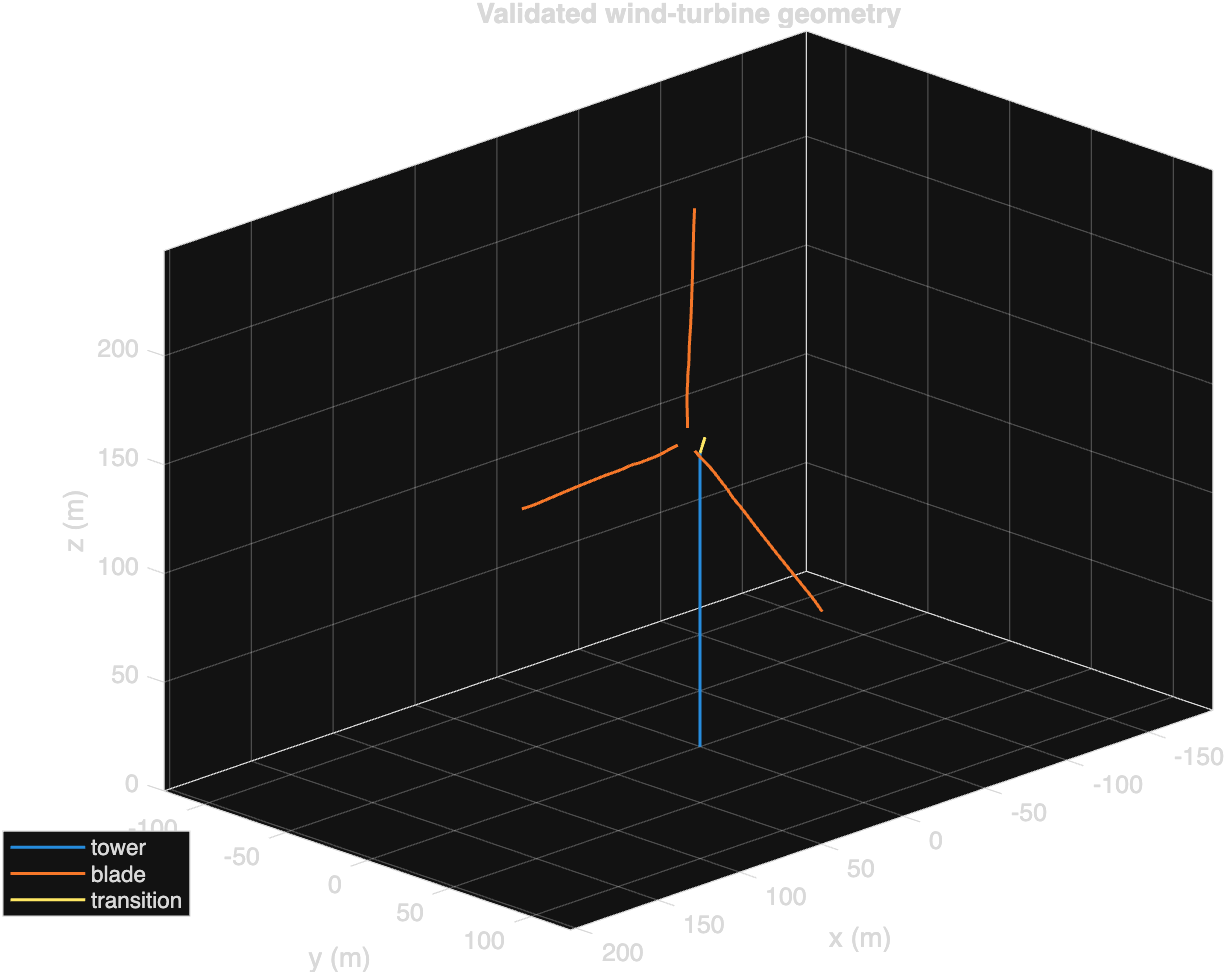
\includegraphics[width=\textwidth,height=0.69\textheight,keepaspectratio]{01_geometria_modelo.png}
\caption{Geometría heredada convertida. Se conservan torre, tres palas, góndola/rotor y transiciones; se eliminan solo los cuatro conectores de penalización.}
\label{fig:resultado-origen-01}
\end{figure}

\begin{figure}[!htbp]
\centering
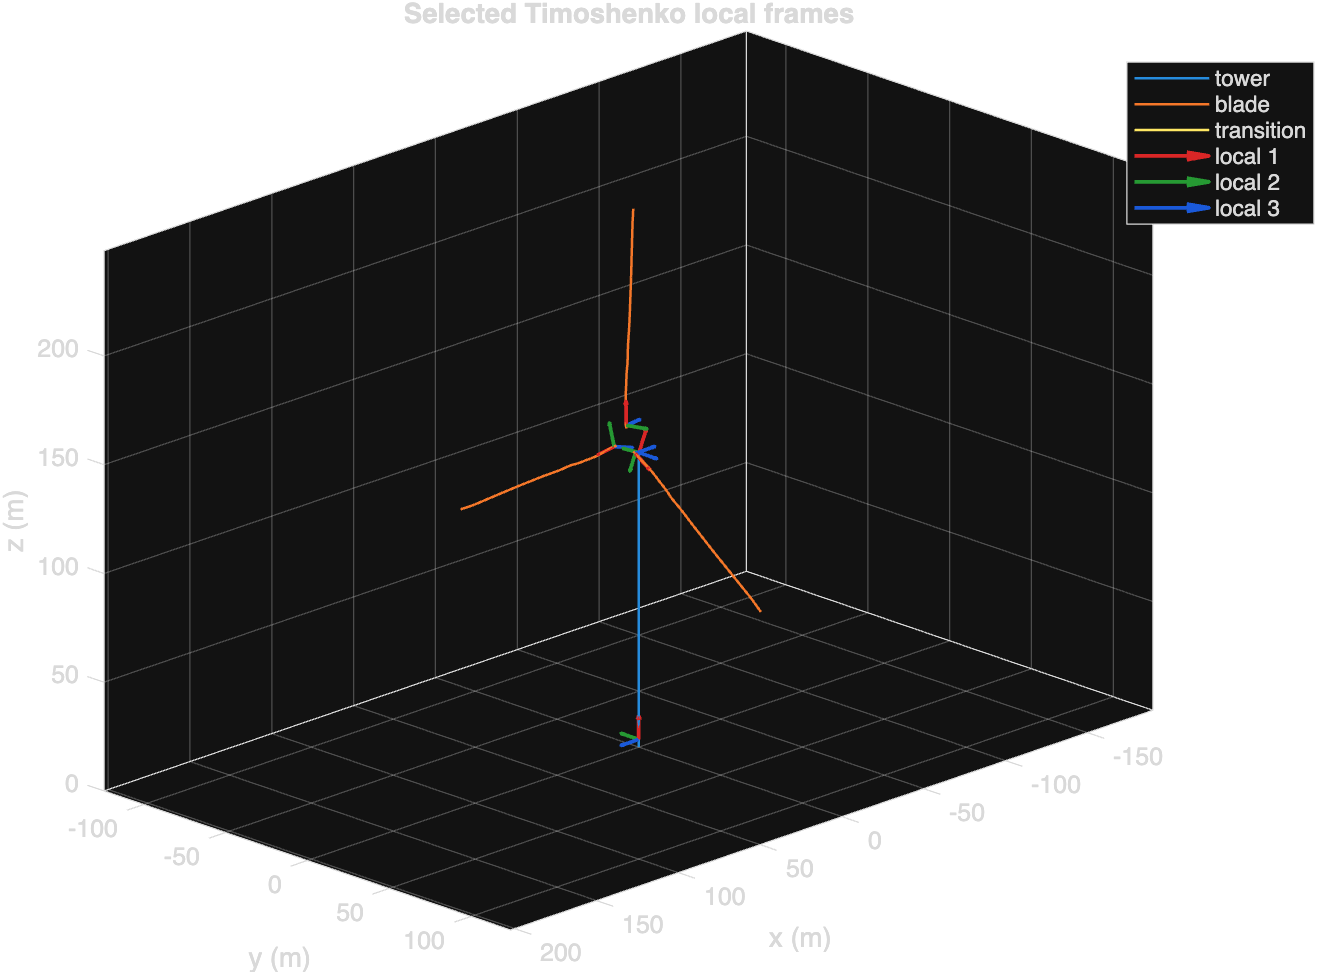
\includegraphics[width=\textwidth,height=0.69\textheight,keepaspectratio]{02_ejes_locales.png}
\caption{Ejes locales obtenidos con auxiliares independientes P1/P2/P3. La orientación no se infiere copiando la de una sola pala.}
\label{fig:resultado-origen-02}
\end{figure}

\begin{figure}[!htbp]
\centering
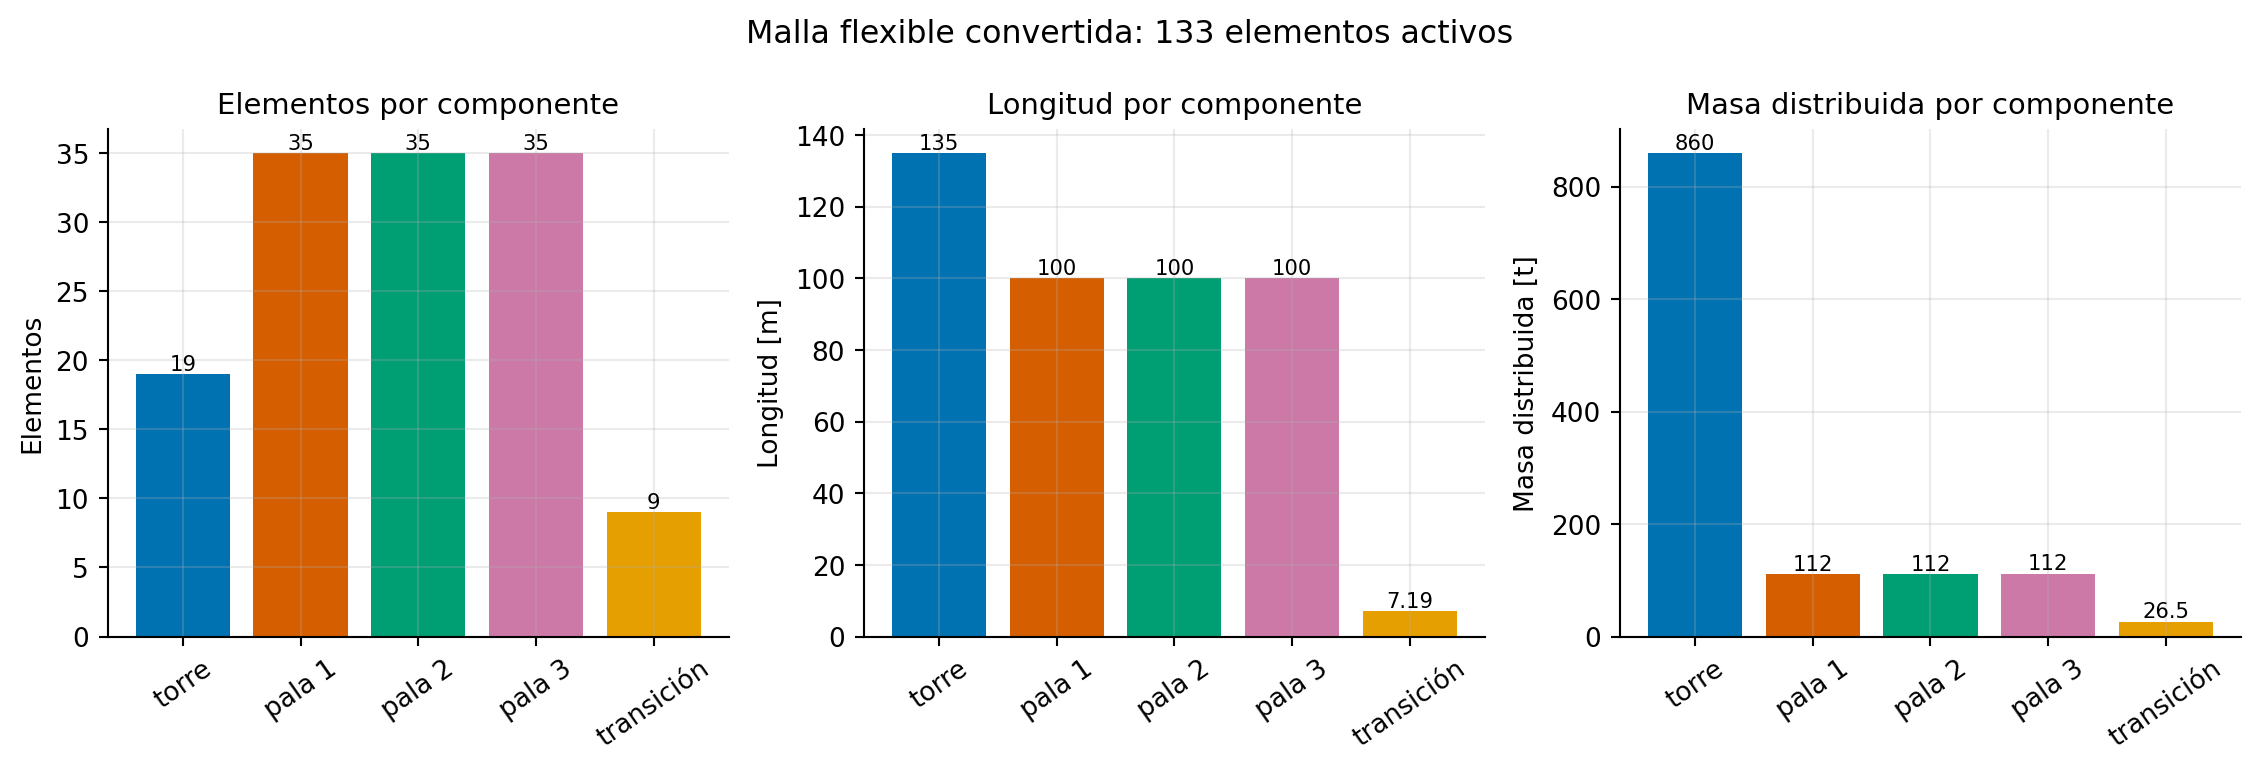
\includegraphics[width=\textwidth,height=0.69\textheight,keepaspectratio]{03_topologia_malla.png}
\caption{Recuento, longitud y masa distribuida por componente. Las 105 vigas de pala se dividen en tres conjuntos homólogos de 35.}
\label{fig:resultado-origen-03}
\end{figure}

\subsection{Conversión de secciones}

Las secciones 1--20 corresponden a torre/transición. Se obtienen a partir de \nolinkurl{secc_torre} y las constantes heredadas \texttt{E=2.1e11 Pa}\allowbreak{}, \texttt{nu=0.3}\allowbreak{} y \nolinkurl{rho=7850 kg/m³}. Las secciones 21--55 son las 35 estaciones de pala. Para ellas se conservan directamente las seis rigideces generalizadas \texttt{EA, GAy, GAz, GJ, EIy, EIz}\allowbreak{}; no se inventan un módulo y un área equivalentes.

Version 0 entrega para la masa de pala las columnas \texttt{AXIALD}\allowbreak{}, \texttt{TORDEN}\allowbreak{}, \texttt{INERT2}\allowbreak{} e \texttt{INERT3}\allowbreak{}. Como \texttt{TORDEN=0}\allowbreak{} en todas las estaciones, el dato importado importado deja \texttt{Jx=NaN}\allowbreak{} y obliga a elegir una regla explícita. La configuración empleada usa el teorema de ejes perpendiculares,

\[
J_x=J_y+J_z,
\]

sin intentar deducirlo de \texttt{EA}\allowbreak{}, \texttt{GJ}\allowbreak{} o un módulo efectivo. Version 0 tampoco entrega offsets del centroide; se documenta \texttt{ycg=zcg=0}\allowbreak{} como supuesto.

\subsection{Distinción entre conversión y convergencia de malla}

La conversión anterior reproduce la topología disponible. El estudio de convergencia es un análisis separado: usa una \textbf{viga uniforme sintética de 12 m} discretizada con 1, 2, 4, 8, 16, 32 y 64 elementos. Esta separación es importante: el refinamiento sintético caracteriza el elemento sin inventar estaciones adicionales dentro de la turbina heredada. No se ha realizado todavía una campaña de refinamiento geométrico de la turbina completa con propiedades interpoladas.

\section{Formulación elemental Timoshenko 3D}

\subsection{Cinemática, ejes y energía}

Cada nodo tiene seis GDL ordenados como tres traslaciones y tres rotaciones. Para el elemento de dos nodos, $\bm q_e$ tiene 12 componentes. El eje local $\bm e_1$ va de I a J. El vector hacia el punto auxiliar se proyecta sobre el plano normal a $\bm e_1$ para definir $\bm e_3$, y la base dextrógira se completa con $\bm e_2=\bm e_3\times\bm e_1$.

La deformación generalizada reúne axial, dos cortantes, torsión y dos curvaturas. La energía se escribe como

\[
U_e=\frac{1}{2}\int_0^L
\bm\varepsilon(\bm q_e)^T\bm C_{\mathrm{sec}}
\bm\varepsilon(\bm q_e)\,\mathrm dx,
\]

donde $\bm C_{\mathrm{sec}}$ contiene las seis rigideces generalizadas positivas de la sección. La matriz elemental resulta de

\[
\bm K_e=\int_0^L\bm B^T\bm C_{\mathrm{sec}}\bm B\,\mathrm dx,
\qquad
\bm\varepsilon=\bm B\bm q_e.
\]

La formulación cerrada exacta se usa en los resultados de la turbina. La integración selectiva emplea dos puntos de Gauss para los términos normales y uno para cortante, y se usa en el estudio de convergencia espacial.

La masa consistente integra traslación del centroide, inercia rotacional y el acoplamiento que produciría una excentricidad. No se diagonaliza de forma silenciosa.

\subsection{Demostración de los seis modos del elemento primitivo}

La demostración no se basa solo en observar una gráfica. Se usaron cuatro argumentos complementarios sobre un elemento sintético bien condicionado de longitud 5 m:

\begingroup
\small
\renewcommand{\arraystretch}{1.16}
\begin{center}
\begin{tabularx}{\textwidth}{@{}YYY@{}}
\toprule
\textbf{Propiedad primitiva} & \textbf{Valor} & \textbf{Unidad} \\
\midrule
Longitud \texttt{L}\allowbreak{} & 5 & m \\
Rigidez axial \texttt{EA}\allowbreak{} & \texttt{2.1e9}\allowbreak{} & N \\
Rigideces de cortante \texttt{GAy}\allowbreak{}, \texttt{GAz}\allowbreak{} & \texttt{4.0e8}\allowbreak{}, \texttt{3.0e8}\allowbreak{} & N \\
Rigidez torsional \texttt{GJ}\allowbreak{} & \texttt{1.5e8}\allowbreak{} & N\,$\cdot$\,m$^2$ \\
Rigideces de flexión \texttt{EIy}\allowbreak{}, \texttt{EIz}\allowbreak{} & \texttt{8.0e7}\allowbreak{}, \texttt{6.0e7}\allowbreak{} & N\,$\cdot$\,m$^2$ \\
Masa lineal \texttt{m}\allowbreak{} & 25 & kg/m \\
Inercias lineales \texttt{Jx}\allowbreak{}, \texttt{Jy}\allowbreak{}, \texttt{Jz}\allowbreak{} & 2.0, 1.2, 1.4 & kg\,$\cdot$\,m \\
Offset del centro de masa \texttt{ycg}\allowbreak{}, \texttt{zcg}\allowbreak{} & 0, 0 & m \\
\bottomrule
\end{tabularx}
\end{center}
\endgroup

Estos valores no representan una sección particular de la turbina: forman un caso unitario reproducible, positivo y sin excentricidad, elegido para aislar la estructura algebraica del elemento.

\begin{enumerate}
\item \textbf{Conteo cinemático.} Hay 12 coordenadas nodales y seis deformaciones independientes. Un movimiento euclídeo 3D posee tres traslaciones y tres rotaciones; por tanto, el subespacio rígido esperado tiene dimensión 6.
\item \textbf{Construcción explícita.} Se construyó $Q\in\mathbb{R}^{12\times6}$ con tres traslaciones uniformes y tres rotaciones infinitesimales, usando $u(x)=t+\theta\times x$ y la misma rotación $\theta$ en ambos nodos. El residuo energético normalizado fue $\lVert KQ\rVert/(\lVert K\rVert\lVert Q\rVert)=2.691\times10^{-18}$.
\end{enumerate}

En bloques de tres componentes y con el orden nodal $q_e=[u_i,\theta_i,u_j,\theta_j]^T$, la base rígida utilizada es

\[
Q=\begin{bmatrix}
I_3 & -[x_i]_\times\\
0   & I_3\\
I_3 & -[x_j]_\times\\
0   & I_3
\end{bmatrix},
\qquad
u_k=t+\theta\times x_k=t-[x_k]_\times\theta.
\]

Para el sistema local primitivo se tomó $x_i=0$ y $x_j=L e_1$. Las seis columnas de $Q$ son linealmente independientes, no producen deformación y por eso deben pertenecer al núcleo de $K$. La SVD demuestra además que el núcleo no contiene ninguna dirección adicional.

\begin{enumerate}
\setcounter{enumi}{2}
\item \textbf{Rango--nulidad.} La SVD normalizada de \texttt{K}\allowbreak{} muestra seis valores singulares materiales y seis nulos: \texttt{rank(K)=6}\allowbreak{}, \texttt{nullity(K)=6}\allowbreak{}. Como la matriz de masa es definida positiva por Cholesky, el problema generalizado no puede ocultar coordenadas sin masa. En la corrida reproducida, \texttt{cholFlag=0}\allowbreak{} y \texttt{min(eig(M))=1.5311}\allowbreak{}, ambos consistentes con \texttt{M}\allowbreak{} definida positiva.
\item \textbf{Espectro generalizado.} Al resolver $\bm K\bm\phi_i=\mu_i\bm M\bm\phi_i$ sin formar $\bm M^{-1}$ aparecen seis valores numéricamente nulos, todos con $|f|\leq1.596\times10^{-5}\,\mathrm{Hz}$, por debajo de la tolerancia $10^{-4}\,\mathrm{Hz}$, y luego seis frecuencias positivas. No aparece ningún autovalor materialmente negativo. Los modos se normalizan con $\bm\phi_i^H\bm M\bm\phi_i=1$.
\end{enumerate}

Aquí $\mu=\omega^2$ y, para los autovalores positivos, $f=\sqrt{\mu}/(2\pi)$. Para representar perturbaciones cercanas a cero se conserva el signo de $\mu$ y se grafica $\operatorname{sign}(\mu)\sqrt{|\mu|}/(2\pi)$; este recurso gráfico no convierte los ceros de redondeo en frecuencias físicas.

\begingroup
\small
\renewcommand{\arraystretch}{1.16}
\begin{center}
\begin{tabularx}{\textwidth}{@{}YYY@{}}
\toprule
\textbf{Grupo} & \textbf{Frecuencias [Hz]} & \textbf{Interpretación} \\
\midrule
Modos 1--6 & magnitud máxima \texttt{1.596e-5}\allowbreak{} & ceros numéricos: 3 traslaciones + 3 rotaciones \\
Modos 7--12 & 248.467, 289.364, 783.567, 933.509, 954.930, 1010.603 & seis deformaciones elásticas independientes \\
\bottomrule
\end{tabularx}
\end{center}
\endgroup

Los signos negativos que aparecen en algunos ceros del CSV no representan una inestabilidad: son perturbaciones de redondeo de autovalores cuya magnitud está muchos órdenes por debajo del primer modo flexible.

\begin{figure}[!htbp]
\centering
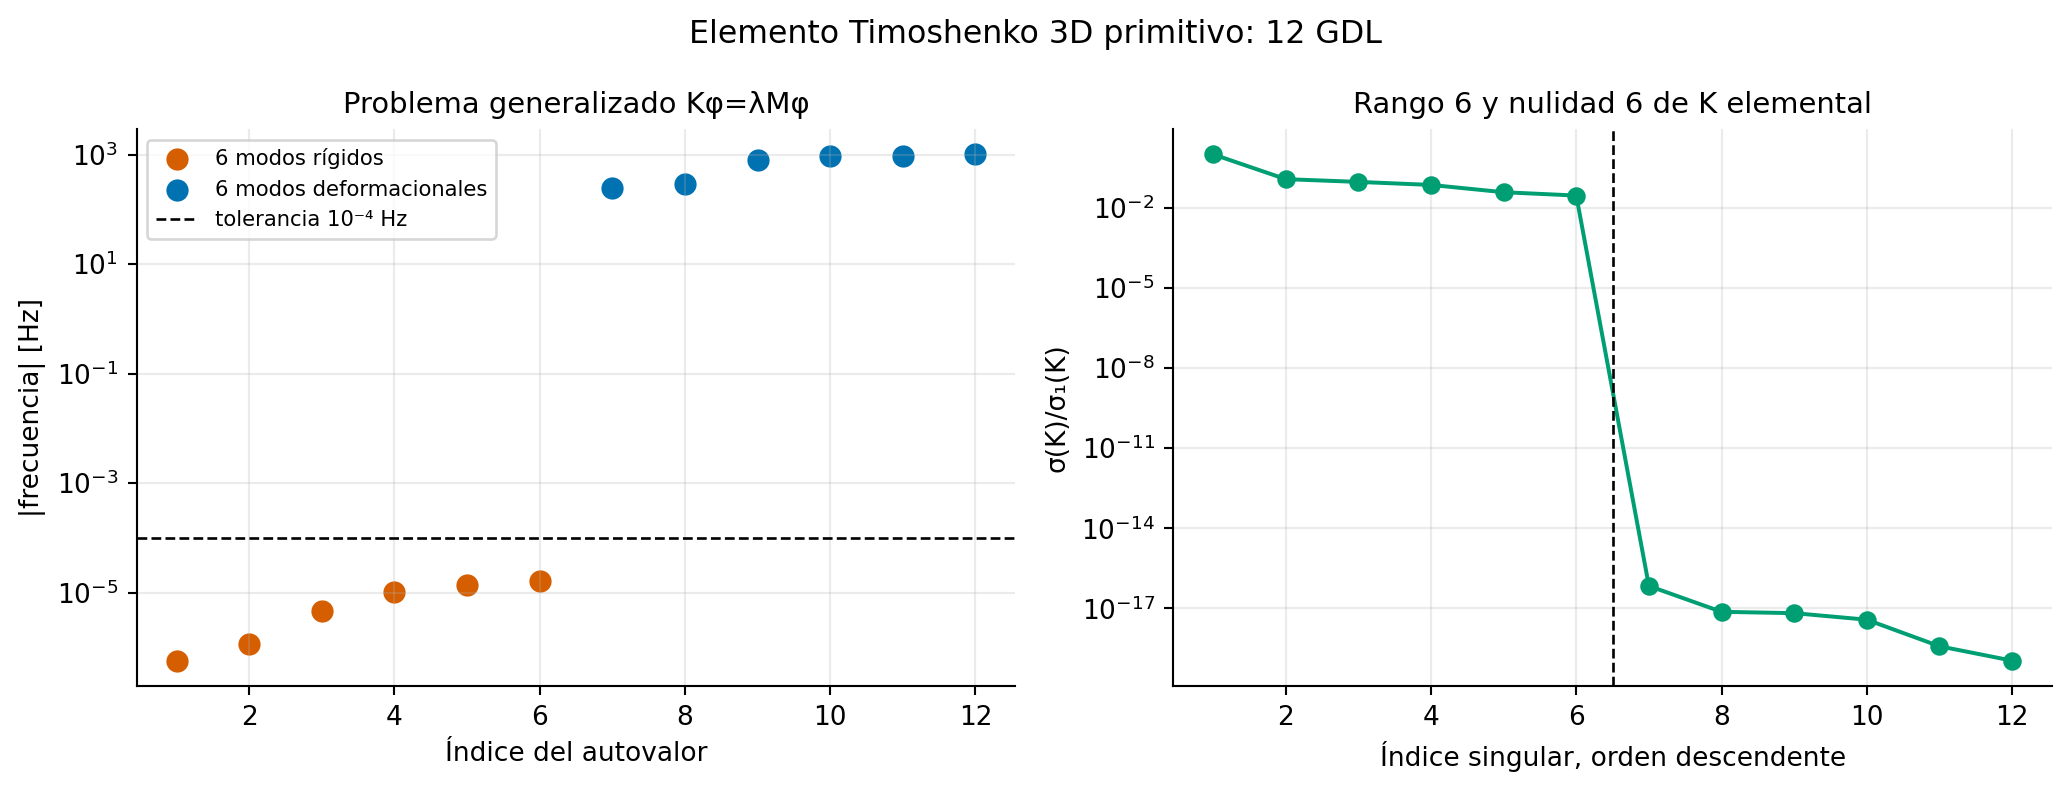
\includegraphics[width=\textwidth,height=0.69\textheight,keepaspectratio]{04_espectro_elemento_primitivo.png}
\caption{A la izquierda se separan los seis ceros de los seis modos deformacionales; a la derecha la SVD demuestra rango 6 y nulidad 6.}
\label{fig:resultado-origen-04}
\end{figure}

\subsection{Extensión a los elementos de la turbina y al modelo global}

El mismo conteo rango--nulidad aplicado a los 133 elementos activos produjo seis direcciones rígidas en cada uno, aun cuando cambian su longitud, orientación y propiedades. La conclusión no depende del elemento sintético ni de una dirección privilegiada.

Para el sistema global se construyó el campo rígido de todos los nodos, se lo proyectó mediante las MPC y se comprobaron energía y compatibilidad. El modelo libre--libre usado para este estudio incluye el constitutivo de tren de referencia para que los maestros 129 y 130 formen un único sistema conectado.

\begingroup
\scriptsize
\renewcommand{\arraystretch}{1.16}
\begin{center}
\begin{tabularx}{\textwidth}{@{}YYYYY@{}}
\toprule
\textbf{Caso} & \textbf{Coordenadas} & \textbf{Ceros} & \textbf{Máximo \nolinkurl{|f_cero|}} & \textbf{Primera frecuencia flexible} \\
\midrule
Elemento primitivo & 12 & 6 & \texttt{1.596e-5 Hz}\allowbreak{} & \texttt{248.467 Hz}\allowbreak{} \\
Turbina conectada libre--libre & 810 & 6 & \texttt{9.662e-7 Hz}\allowbreak{} & \texttt{0.372022 Hz}\allowbreak{} \\
Misma turbina con base fija & 804 & 0 & 0 & \texttt{0.167768 Hz}\allowbreak{} \\
\bottomrule
\end{tabularx}
\end{center}
\endgroup

En el caso libre--libre, el residuo rígido de energía fue \texttt{2.788e-19}\allowbreak{} y el de compatibilidad con \texttt{Tc}\allowbreak{}, \texttt{3.317e-17}\allowbreak{}. El séptimo autovalor ya es flexible. Al retirar los seis GDL de apoyo del nodo 1, ninguno de los 18 autovalores menores evaluados es nulo. Esto demuestra simultáneamente conectividad global y ausencia de mecanismos espurios dentro del rango examinado.

\begin{figure}[!htbp]
\centering
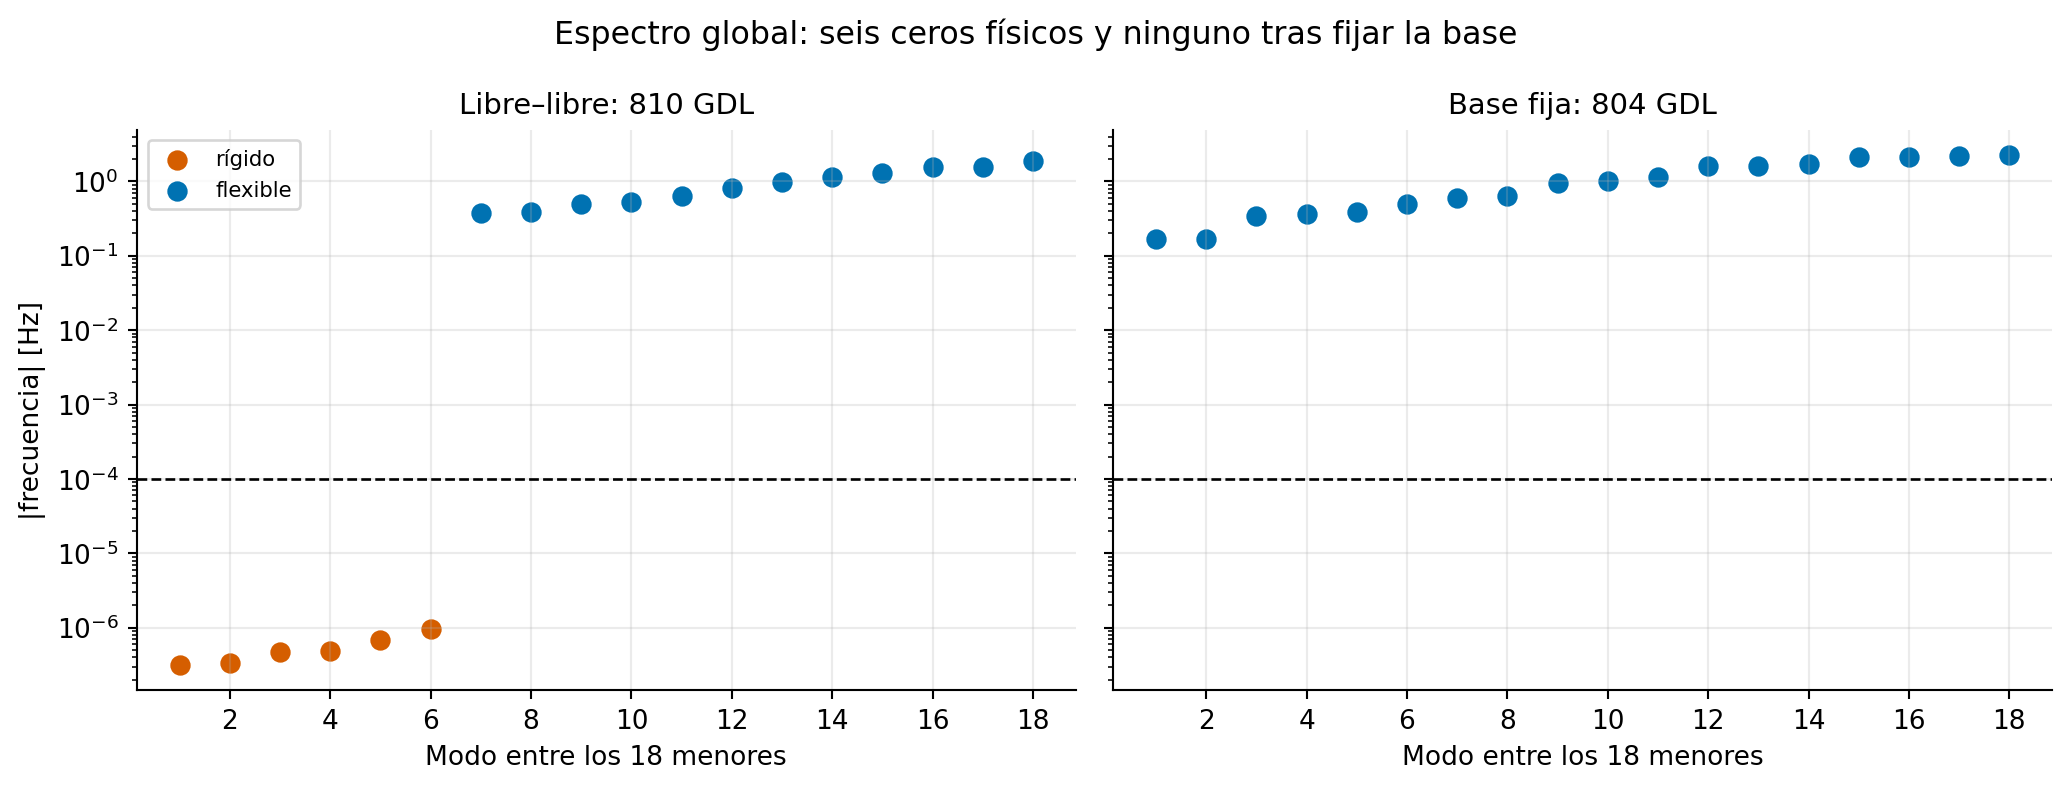
\includegraphics[width=\textwidth,height=0.69\textheight,keepaspectratio]{05_espectro_global_modos_rigidos.png}
\caption{Seis ceros en el ensamblaje libre--libre y cero mecanismos después de empotrar la base.}
\label{fig:resultado-origen-05}
\end{figure}

\section{Restricciones exactas, grados de libertad y masas}

\subsection{MPC y apoyo}

La relación cinemática entre las coordenadas nodales completas y las independientes se escribe

\[
\bm q_{\mathrm{full}}=\bm T_c\,\bar{\bm q},
\qquad
\bar{\bm M}=\bm T_c^T\bm M_{\mathrm{full}}\bm T_c,
\qquad
\bar{\bm K}=\bm T_c^T\bm K_{\mathrm{full}}\bm T_c.
\]

El nodo 129 es maestro de la góndola y el 130 maestro del rotor. Las raíces 21, 57 y 93 son esclavas del nodo 130 con sus brazos geométricos. Cada raíz elimina seis coordenadas dependientes: \texttt{828-18=810}\allowbreak{}. La base fija elimina después las seis coordenadas del nodo 1: quedan 804 GDL de análisis.

$\bm T_c$ tiene tamaño $828\times810$, 846 entradas no nulas y rango numérico 810. La condensación elimina solamente las 18 coordenadas esclavas y preserva el brazo rígido entre el cubo y cada raíz. No se usa una rigidez de penalización, de modo que no se introduce una frecuencia artificial asociada a un resorte excesivamente rígido.

\begin{figure}[!htbp]
\centering
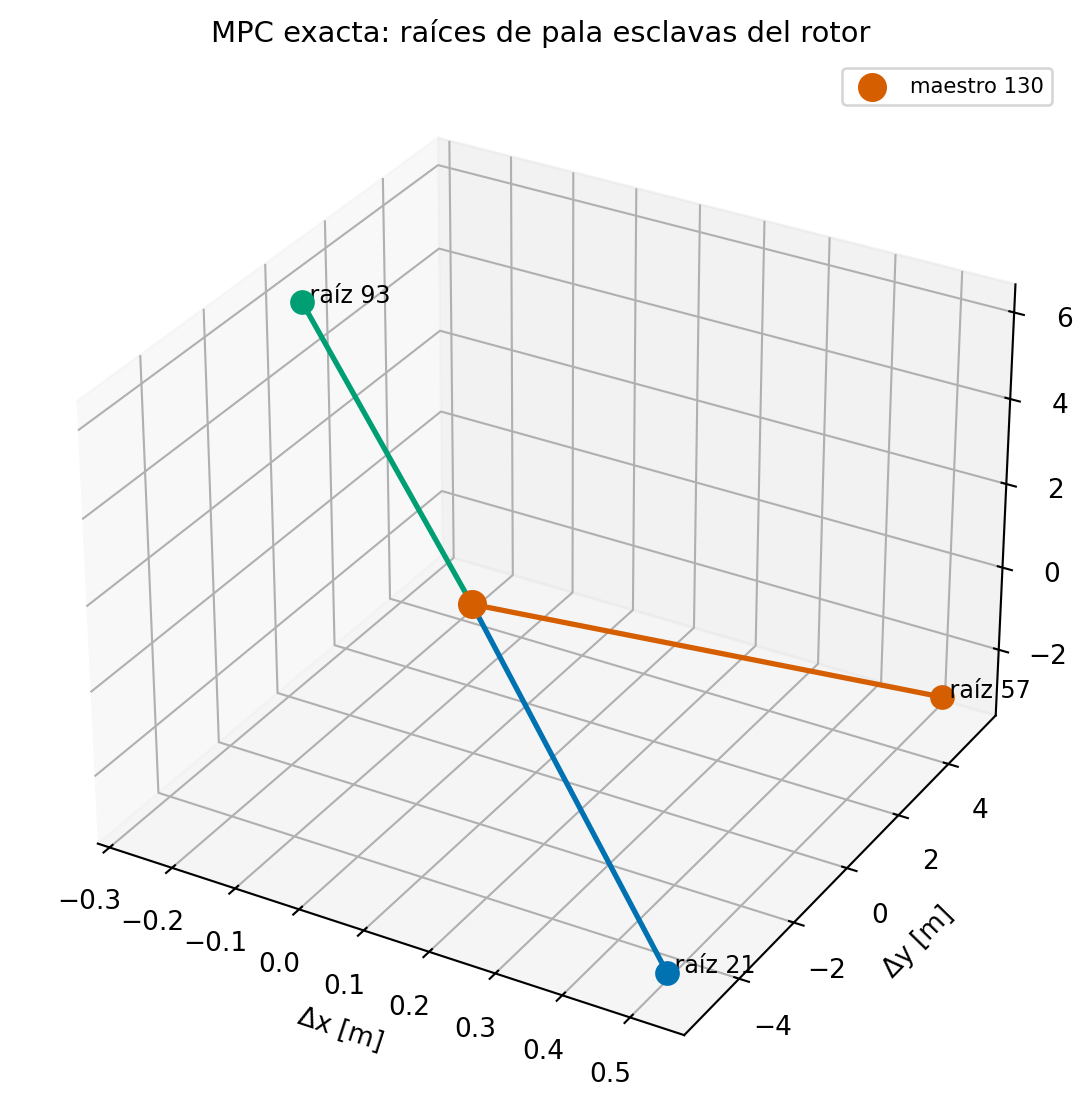
\includegraphics[width=\textwidth,height=0.69\textheight,keepaspectratio]{10_geometria_restricciones_mpc.png}
\caption{Brazos desde el maestro del rotor hacia las tres raíces esclavas.}
\label{fig:resultado-origen-10}
\end{figure}

\begin{figure}[!htbp]
\centering
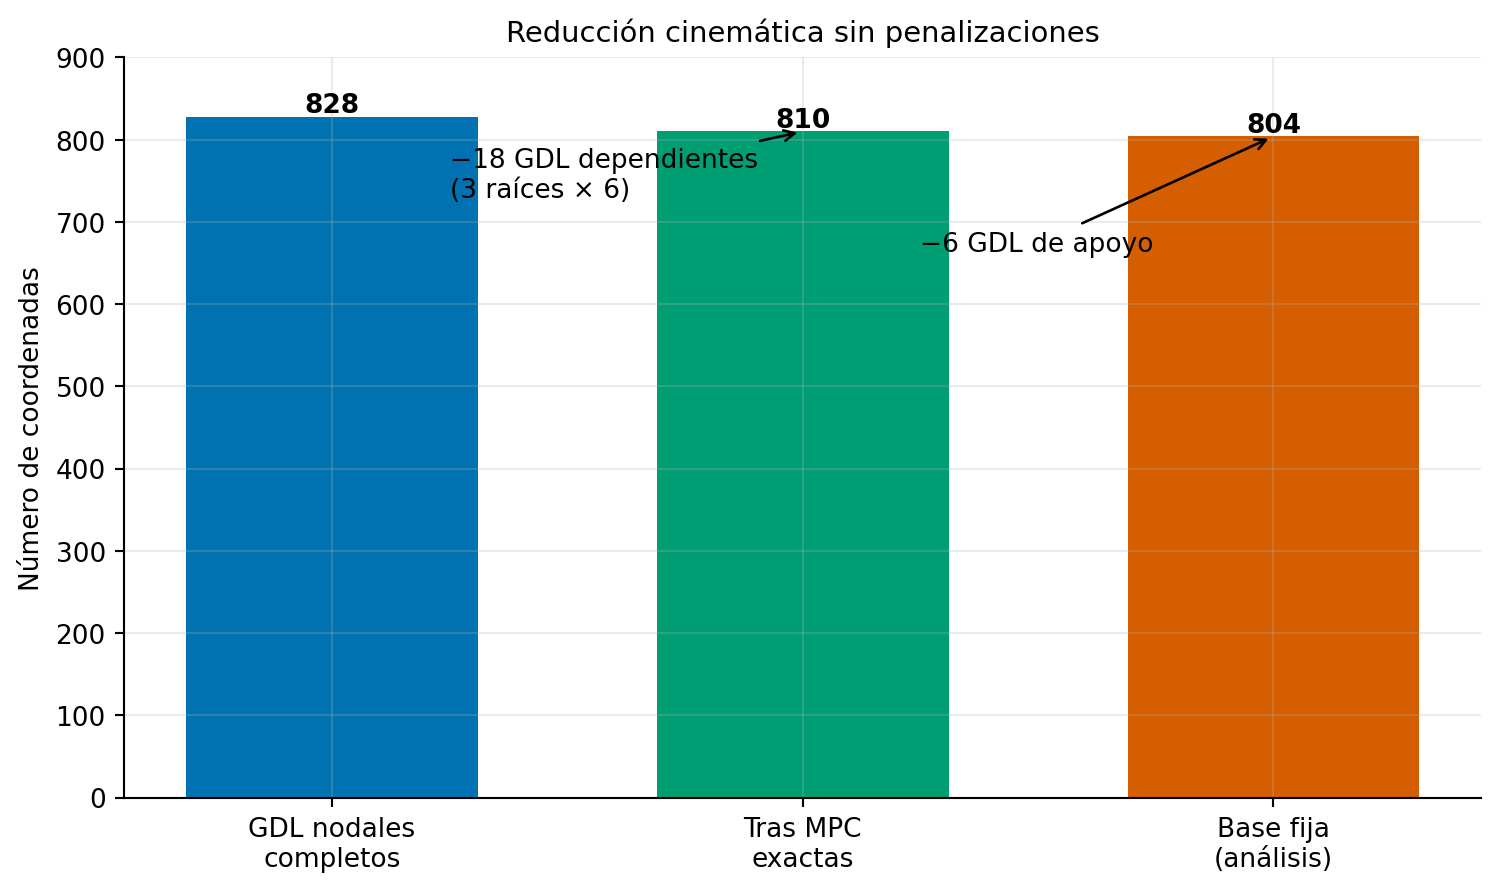
\includegraphics[width=\textwidth,height=0.69\textheight,keepaspectratio]{11_reduccion_grados_libertad.png}
\caption{Paso de 828 GDL nodales a 810 independientes y 804 de análisis.}
\label{fig:resultado-origen-11}
\end{figure}

\subsection{Masas distribuidas y cuerpos rígidos}

\begingroup
\small
\renewcommand{\arraystretch}{1.16}
\begin{center}
\begin{tabularx}{\textwidth}{@{}YY@{}}
\toprule
\textbf{Contribución} & \textbf{Masa [kg]} \\
\midrule
Torre & 859,784.72 \\
Pala 1 & 111,605.61 \\
Pala 2 & 111,608.51 \\
Pala 3 & 111,623.52 \\
Transiciones & 26,488.80 \\
Góndola & 1,184,500.00 \\
Cubo & 196,000.00 \\
\textbf{Total} & \textbf{2,601,611.15} \\
\bottomrule
\end{tabularx}
\end{center}
\endgroup

La masa distribuida suma 1,221,111.15 kg y los cuerpos rígidos 1,380,500 kg. El CG global calculado es \nolinkurl{[0.460663, 2.251e-6, 113.886566] m}. La orientación de la góndola conserva el tensor completo, incluido \texttt{Jxz=1.551199e6 kg\,$\cdot$\,m$^2$}\allowbreak{}. Los offsets \texttt{rCG}\allowbreak{} se mantienen en cero porque el legado no proporciona un dato disponible; esta colocalización es una hipótesis visible.

\begin{figure}[!htbp]
\centering
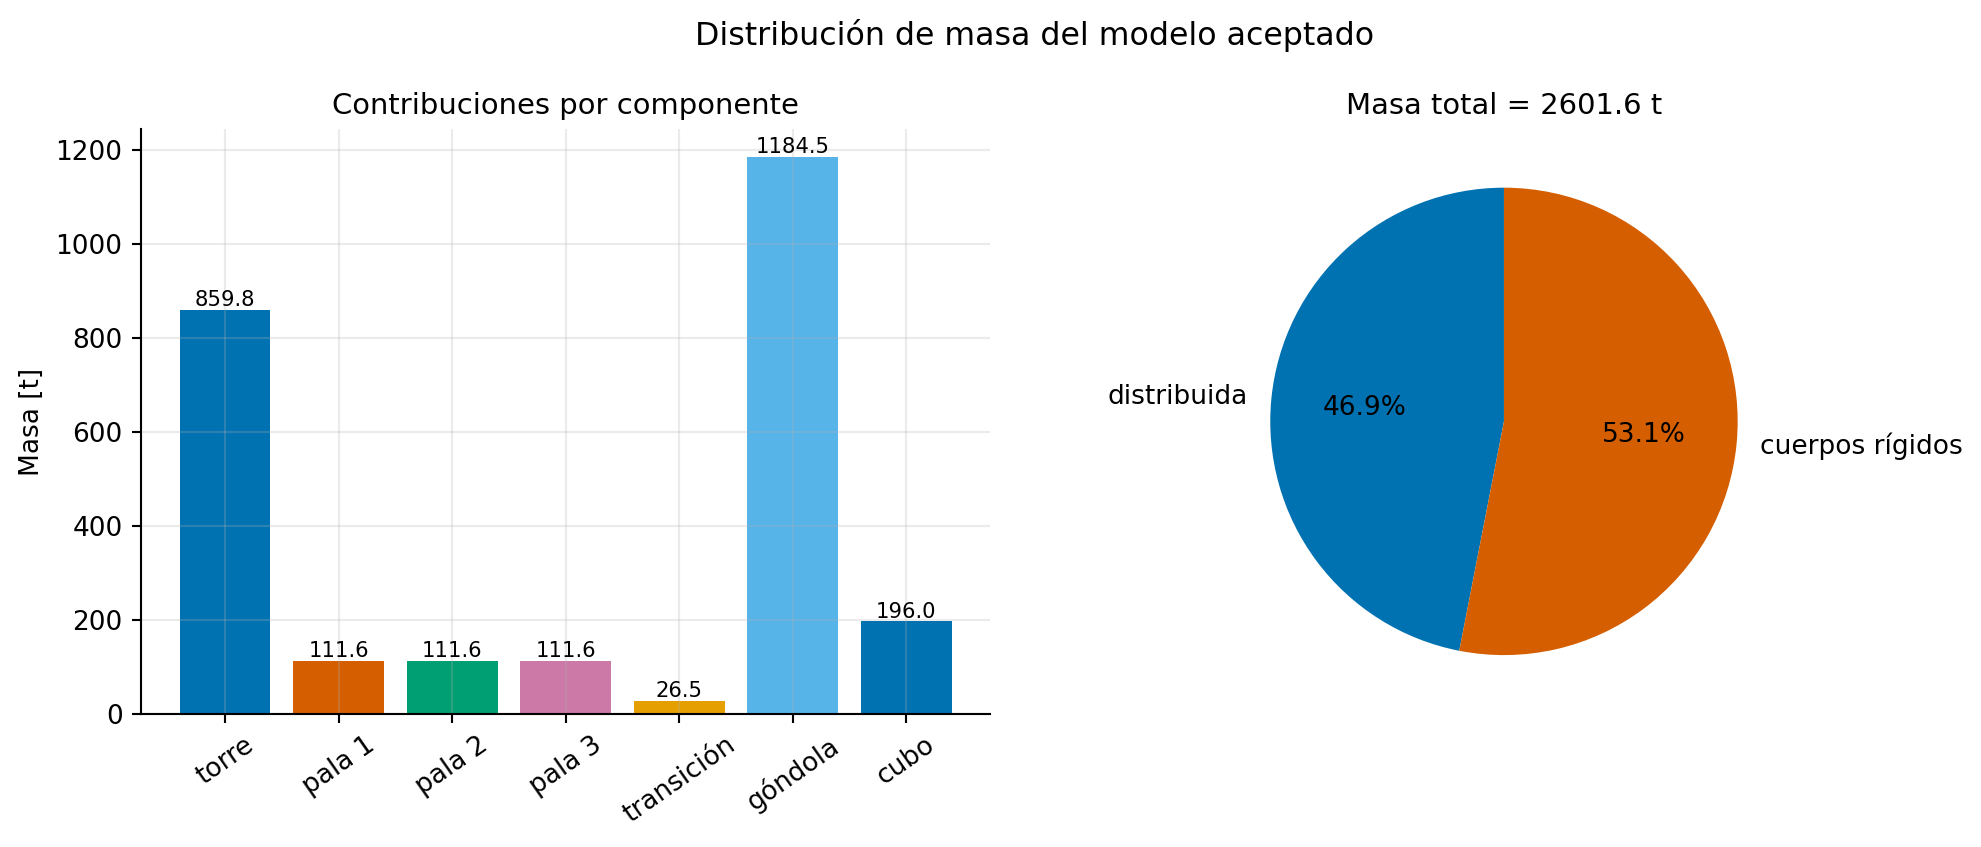
\includegraphics[width=\textwidth,height=0.69\textheight,keepaspectratio]{12_descomposicion_masa.png}
\caption{La góndola domina la masa concentrada; la masa flexible sigue siendo una fracción importante y se integra elemento a elemento.}
\label{fig:resultado-origen-12}
\end{figure}

\subsection{Sensibilidad a la formulación de masa}

La matriz consistente es la opción de producción. HRZ se implementó solo como comparación. Ambas conservan la masa total, pero HRZ cambia levemente el CG y las frecuencias: en ocho modos de torre la diferencia máxima fue 1.0738\% y el MAC mínimo después de asociar ramas fue 0.911563. Por ello, las frecuencias publicadas en el resto del informe corresponden a la masa consistente; HRZ se muestra únicamente como sensibilidad a la redistribución de masa.

\begin{figure}[!htbp]
\centering
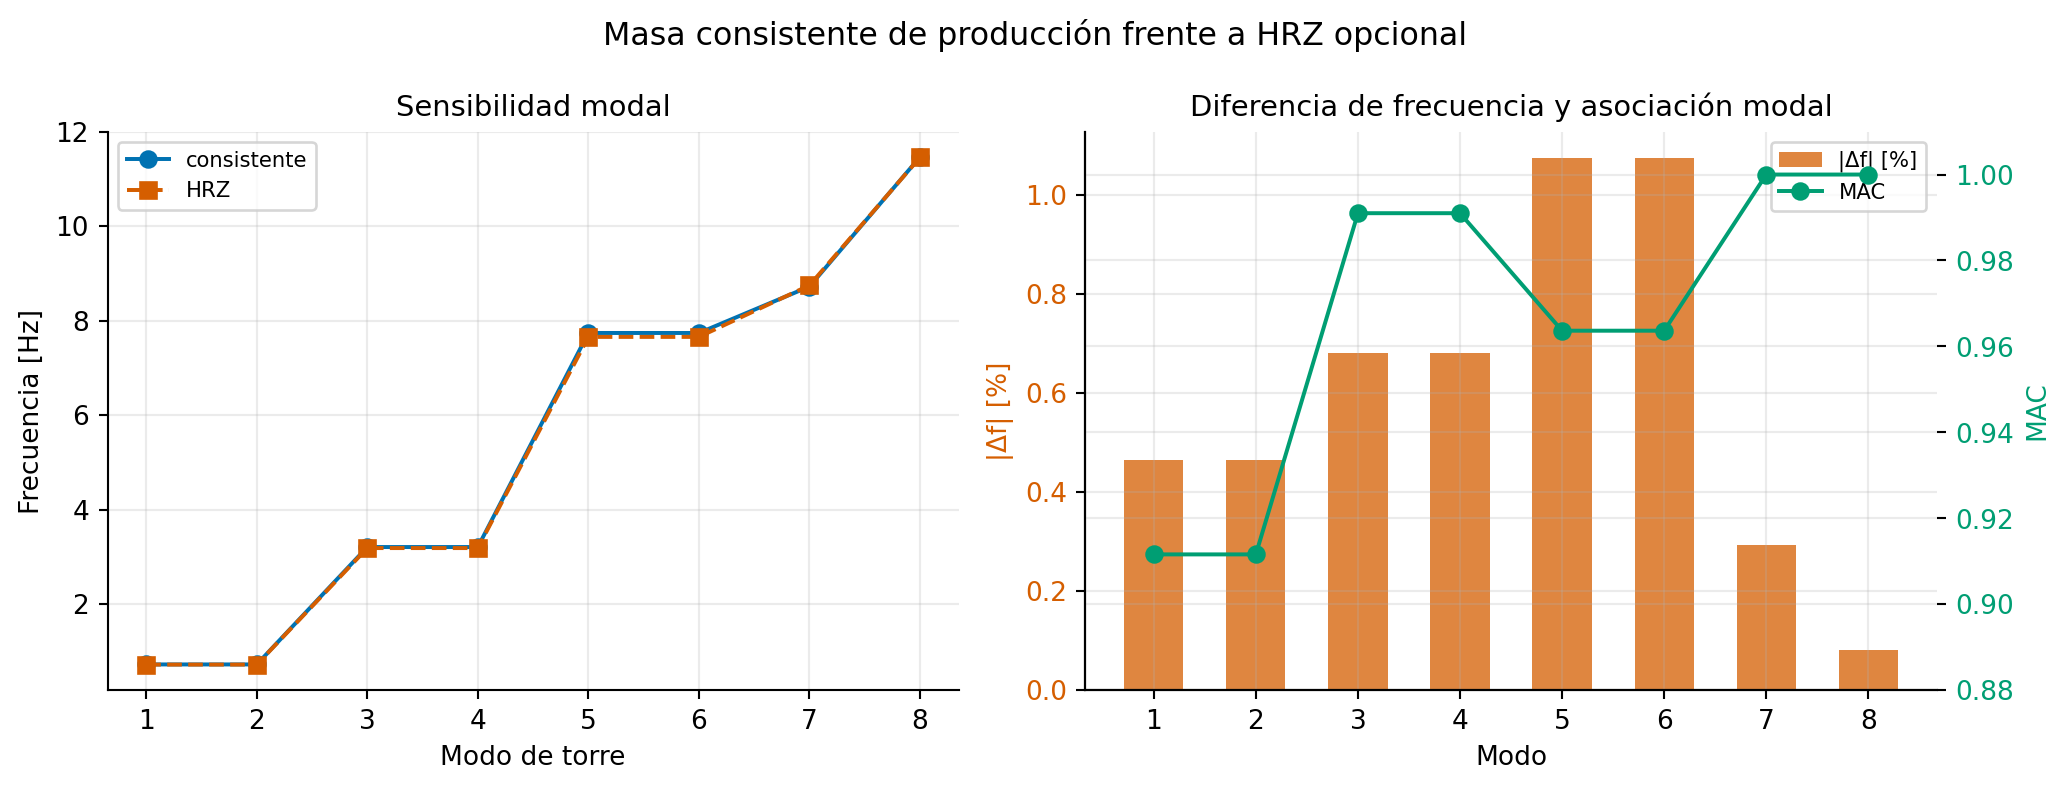
\includegraphics[width=\textwidth,height=0.69\textheight,keepaspectratio]{13_comparacion_masa_consistente_hrz.png}
\caption{HRZ conserva la masa traslacional, pero altera la distribución y por tanto el espectro. La diferencia cuantifica sensibilidad, no incertidumbre física completa.}
\label{fig:resultado-origen-13}
\end{figure}

\section{Convergencia espacial y resultados de subsistemas}

\subsection{Caso analítico de viga uniforme}

El caso usa una viga uniforme de 12 m, integración selectiva y referencias analíticas para desplazamiento de punta y frecuencias de flexión. A 64 elementos se obtuvo:

\begingroup
\small
\renewcommand{\arraystretch}{1.16}
\begin{center}
\begin{tabularx}{\textwidth}{@{}YYYY@{}}
\toprule
\textbf{Magnitud} & \textbf{Resultado} & \textbf{Error relativo} & \textbf{Criterio esperado} \\
\midrule
Desplazamiento de punta & \texttt{9.59944e-6 m}\allowbreak{} & \texttt{6.103e-5}\allowbreak{} & \texttt{1e-3}\allowbreak{} \\
Primera frecuencia & \texttt{6.02046 Hz}\allowbreak{} & \texttt{3.643e-5}\allowbreak{} & \texttt{1e-3}\allowbreak{} \\
Segunda frecuencia & \texttt{37.75024 Hz}\allowbreak{} & \texttt{5.838e-4}\allowbreak{} & \texttt{1e-3}\allowbreak{} \\
\bottomrule
\end{tabularx}
\end{center}
\endgroup

Con un único elemento, la segunda frecuencia es \texttt{3.248743e6 Hz}\allowbreak{}. Ese valor no es una frecuencia física de la viga: la discretización de un elemento no puede representar la segunda forma de flexión y el autovector disponible se vuelve dominantemente cortante. Su descenso monótono hacia la referencia al refinar es precisamente la evidencia relevante. El primer modo y el desplazamiento también convergen sin mostrar bloqueo por cortante en el régimen probado.

\begin{figure}[!htbp]
\centering
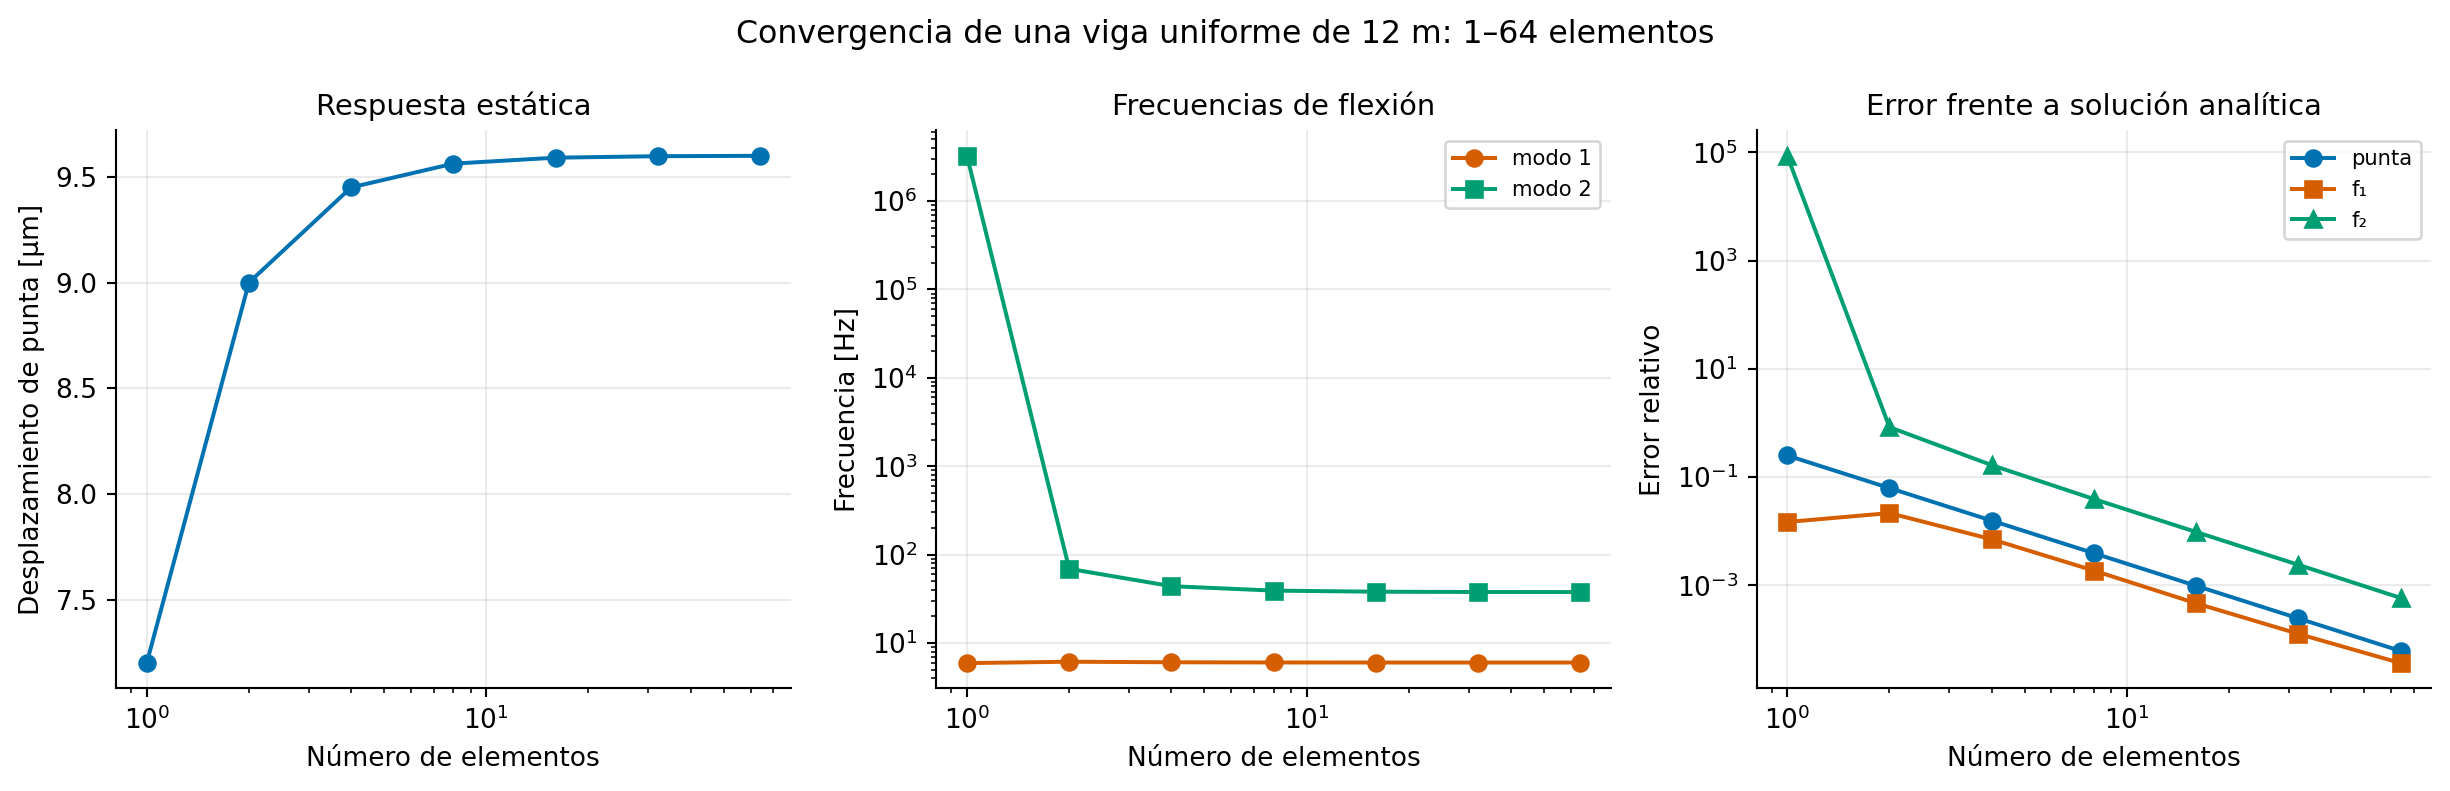
\includegraphics[width=\textwidth,height=0.69\textheight,keepaspectratio]{07_convergencia_malla_detallada.png}
\caption{Desplazamiento, frecuencias y errores relativos frente a las soluciones analíticas para 1--64 elementos.}
\label{fig:resultado-origen-07}
\end{figure}

\subsection{Voladizos aislados}

La torre y cada pala se extrajeron del modelo y se empotraron en su raíz. Así se obtienen frecuencias propias de cada componente antes de ensamblar la turbina:

\begingroup
\small
\renewcommand{\arraystretch}{1.16}
\begin{center}
\begin{tabularx}{\textwidth}{@{}YYYY@{}}
\toprule
\textbf{Subsistema} & \textbf{Longitud [m]} & \textbf{Masa [kg]} & \textbf{Primera frecuencia [Hz]} \\
\midrule
Torre & 135.0000 & 859,784.72 & 0.7196683 \\
Pala 1 & 100.0820 & 111,605.61 & 0.4194612 \\
Pala 2 & 100.0821 & 111,608.51 & 0.4194880 \\
Pala 3 & 100.0899 & 111,623.52 & 0.4194551 \\
\bottomrule
\end{tabularx}
\end{center}
\endgroup

La dispersión relativa máxima entre frecuencias homólogas de las tres palas es \texttt{1.674e-4}\allowbreak{} (0.01674\%), frente a un criterio esperado de \texttt{1e-3}\allowbreak{} (0.1\%). La pequeña diferencia es coherente con las diferencias heredadas de geometría y masa; no indica una separación modal significativa entre palas.

\begin{figure}[!htbp]
\centering
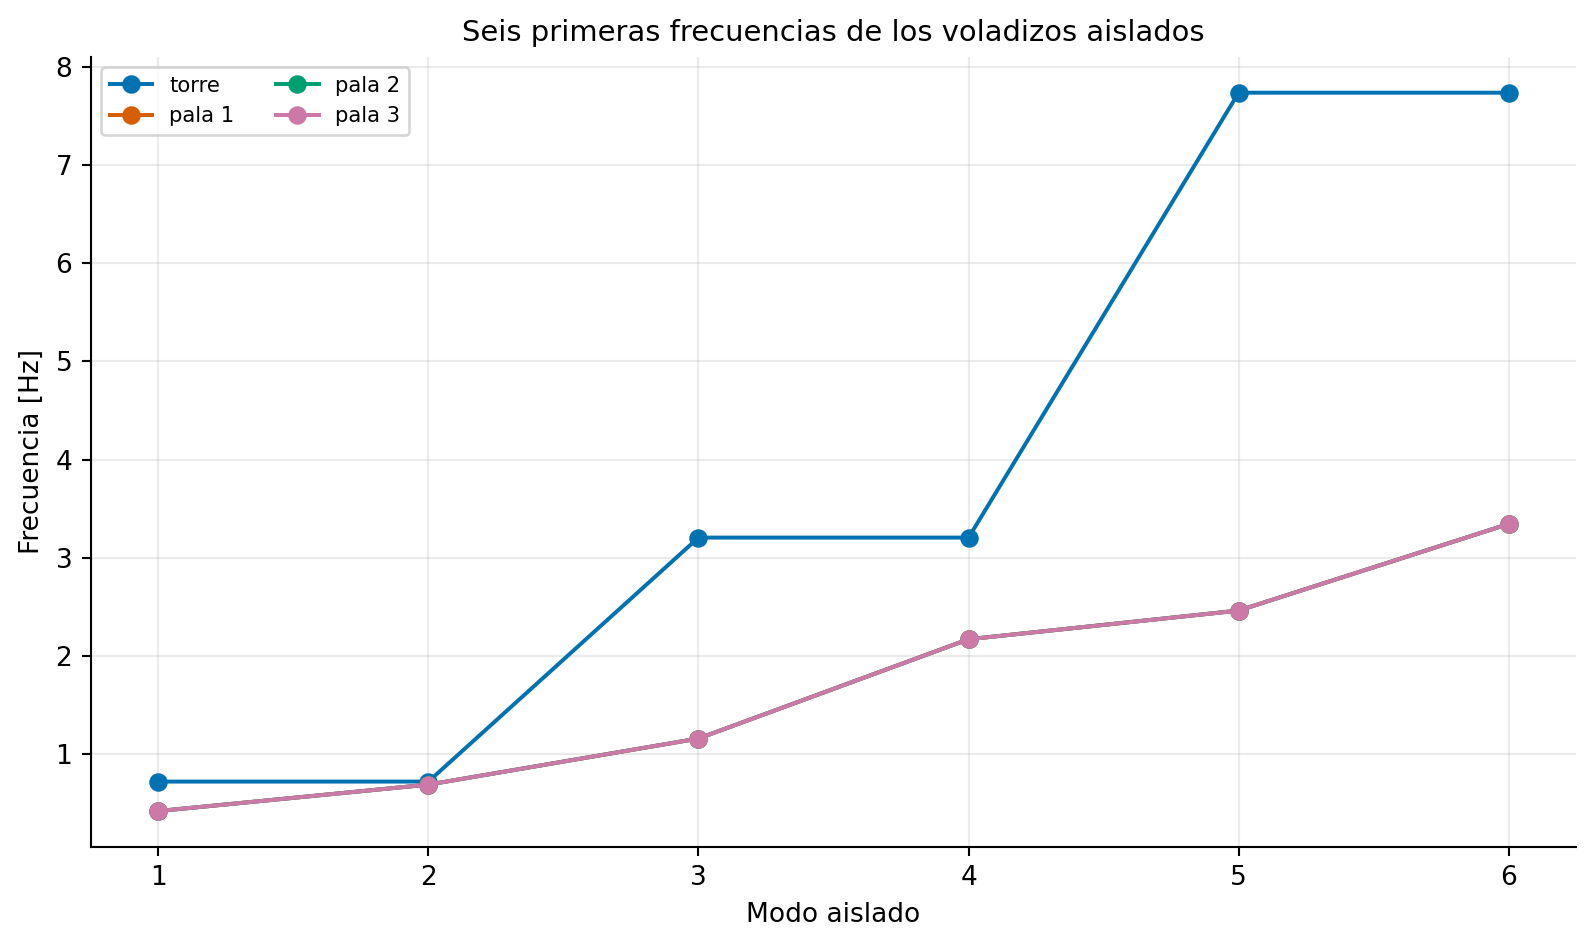
\includegraphics[width=\textwidth,height=0.69\textheight,keepaspectratio]{08_frecuencias_subsistemas_aislados.png}
\caption{Seis primeras frecuencias de torre y palas como voladizos aislados.}
\label{fig:resultado-origen-08}
\end{figure}

\begin{figure}[!htbp]
\centering
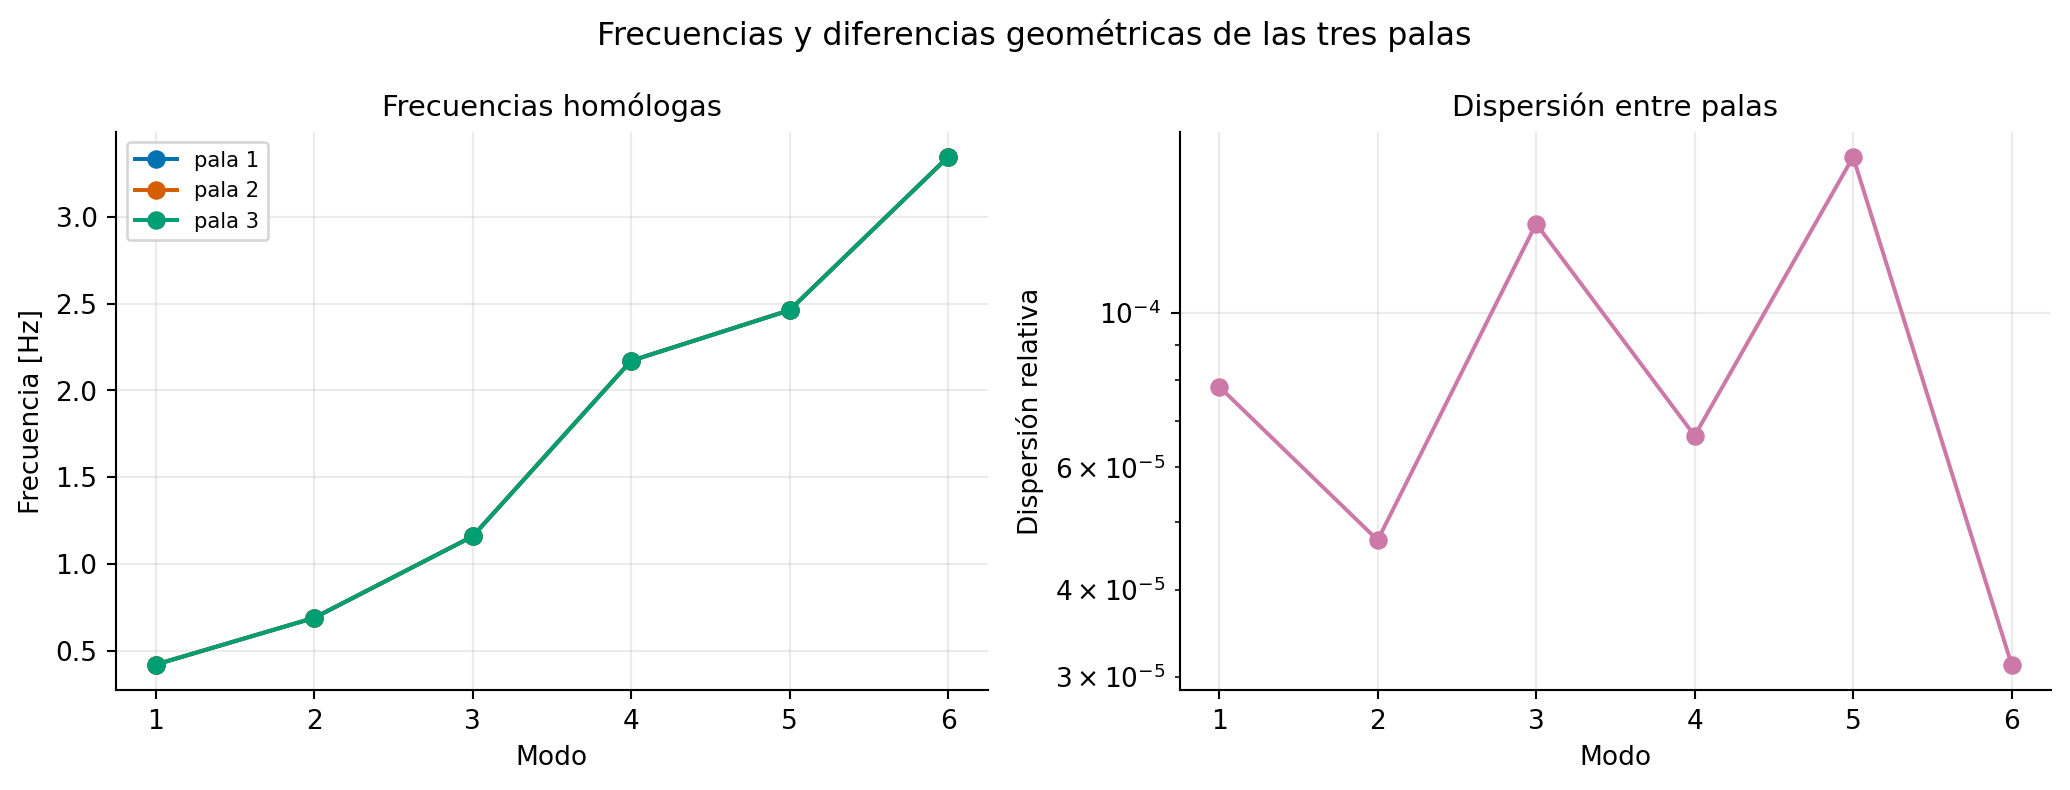
\includegraphics[width=\textwidth,height=0.69\textheight,keepaspectratio]{09_equivalencia_modal_palas.png}
\caption{Coincidencia de frecuencias homólogas y dispersión relativa por modo.}
\label{fig:resultado-origen-09}
\end{figure}

Estas frecuencias no son las de la turbina completa: no incluyen masas rígidas, tren, gravedad, giro ni acoplamiento torre--rotor.

\section{Equilibrio estático, gravedad y centrifugación}

El equilibrio usa una descripción corrotacional. En cada iteración se actualiza el marco del elemento, se separa el movimiento rígido y se evalúa la energía Timoshenko sobre la deformación local. Para una velocidad prescrita $\Omega$, la ecuación no lineal es

\[
\bm r(\bm q;\Omega)
=\bm f_{\mathrm{int}}(\bm q)
-\bm f_g
-\bm f_c(\bm q;\Omega)
-\bm f_a(\bm q,\dot{\bm q})
=\bm 0 .
\]

La actualización de Newton resuelve

\[
\bm K_T(\bm q_k;\Omega)\,\Delta\bm q_k=-\bm r_k,
\qquad
\bm q_{k+1}=\bm q_k+\eta_k\Delta\bm q_k,
\]

donde $0<\eta_k\leq1$ procede de la búsqueda lineal. La continuación $0\rightarrow6\rightarrow12$ RPM reutiliza el estado anterior y evita aplicar de una vez toda la carga centrífuga.

\begingroup
\scriptsize
\renewcommand{\arraystretch}{1.16}
\begin{center}
\begin{tabularx}{\textwidth}{@{}YYYYYY@{}}
\toprule
\textbf{RPM} & \textbf{Iteraciones} & \textbf{Residuo relativo} & \textbf{Criterio esperado} & \textbf{$u_{\max}$ [m]} & \textbf{$\lVert\bm f_c\rVert$ [MN]} \\
\midrule
0 & 5 & \texttt{8.984e-9}\allowbreak{} & $\leq10^{-8}$ & 1.39153 & 0 \\
6 & 5 & \texttt{3.641e-9}\allowbreak{} & $\leq10^{-8}$ & 1.40993 & 0.5466 \\
12 & 6 & \texttt{6.586e-9}\allowbreak{} & $\leq10^{-8}$ & 1.46241 & 2.1867 \\
\bottomrule
\end{tabularx}
\end{center}
\endgroup

La fuerza centrífuga cumple $\bm f_c\propto\Omega^2$: al duplicar la velocidad de 6 a 12 RPM su norma se cuadruplica. La norma de la carga gravitacional es $1.195738\times10^7$ N. El axial de compresión en la base de la torre cambia de aproximadamente $-25.190$ MN a $-25.305$ MN entre 0 y 12 RPM, mientras el máximo axial de tracción en palas crece de 0.573 MN a 7.565 MN. El incremento de $u_{\max}$, de 1.3915 m a 1.4624 m, refleja la combinación entre gravedad, rigidez geométrica y tracción centrífuga.

\begin{figure}[!htbp]
\centering
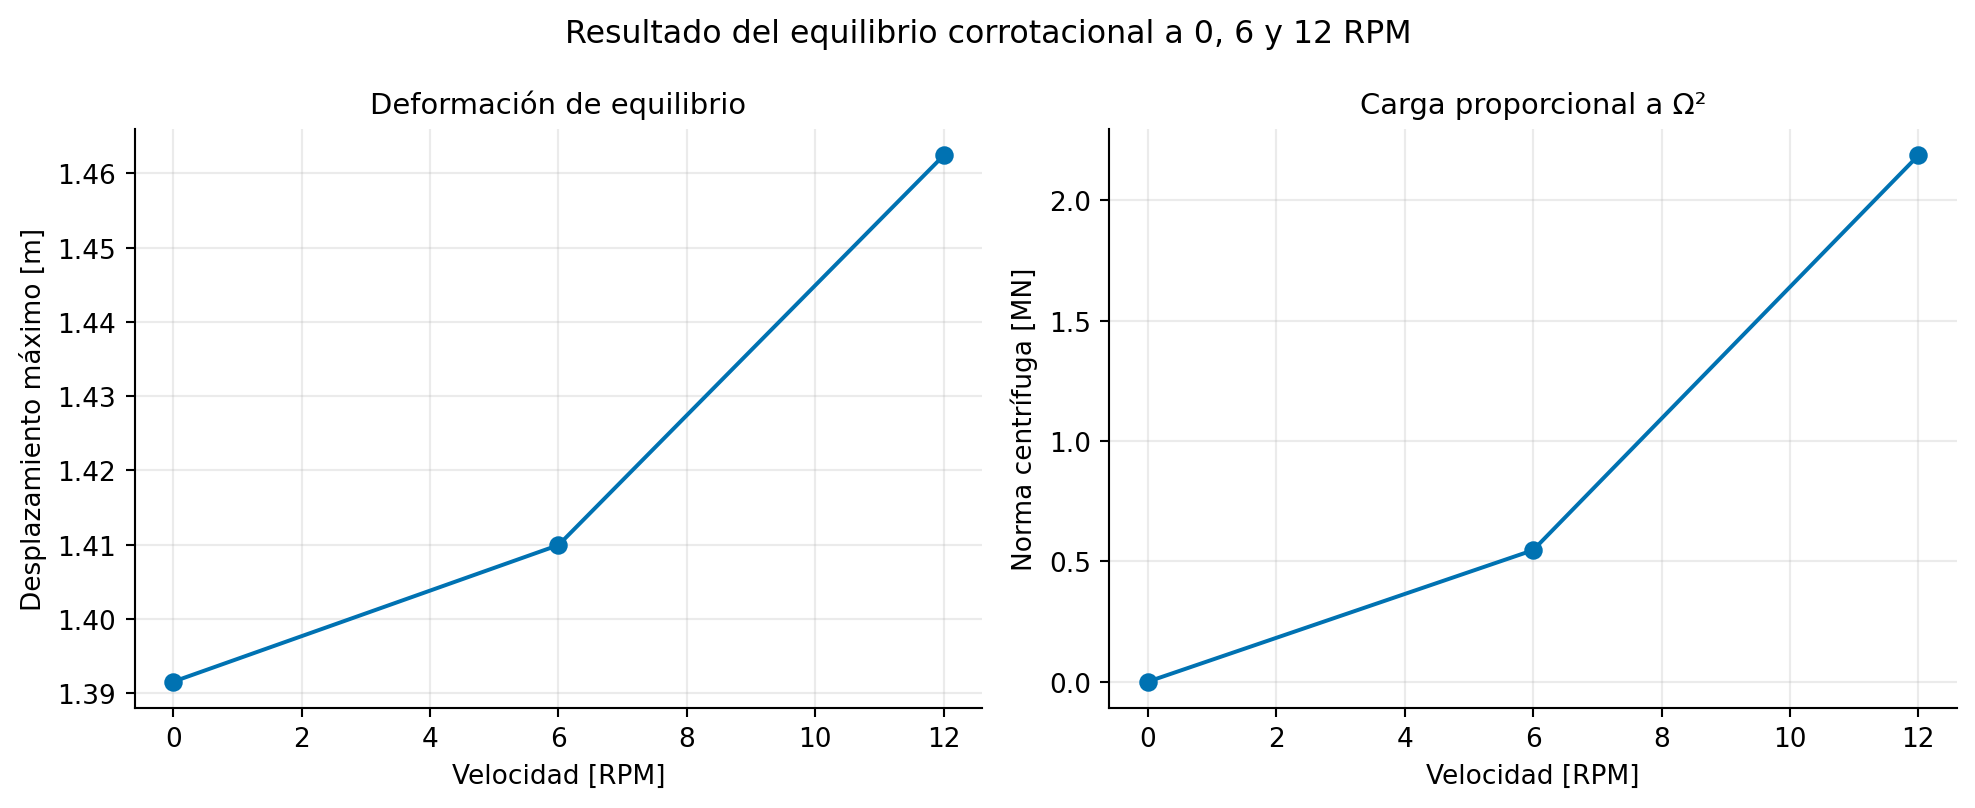
\includegraphics[width=\textwidth,height=0.69\textheight,keepaspectratio]{14_equilibrio_por_velocidad.png}
\caption{Desplazamiento máximo de equilibrio y norma de la carga centrífuga para las tres velocidades prescritas.}
\label{fig:resultado-origen-14}
\end{figure}

\begin{figure}[!htbp]
\centering
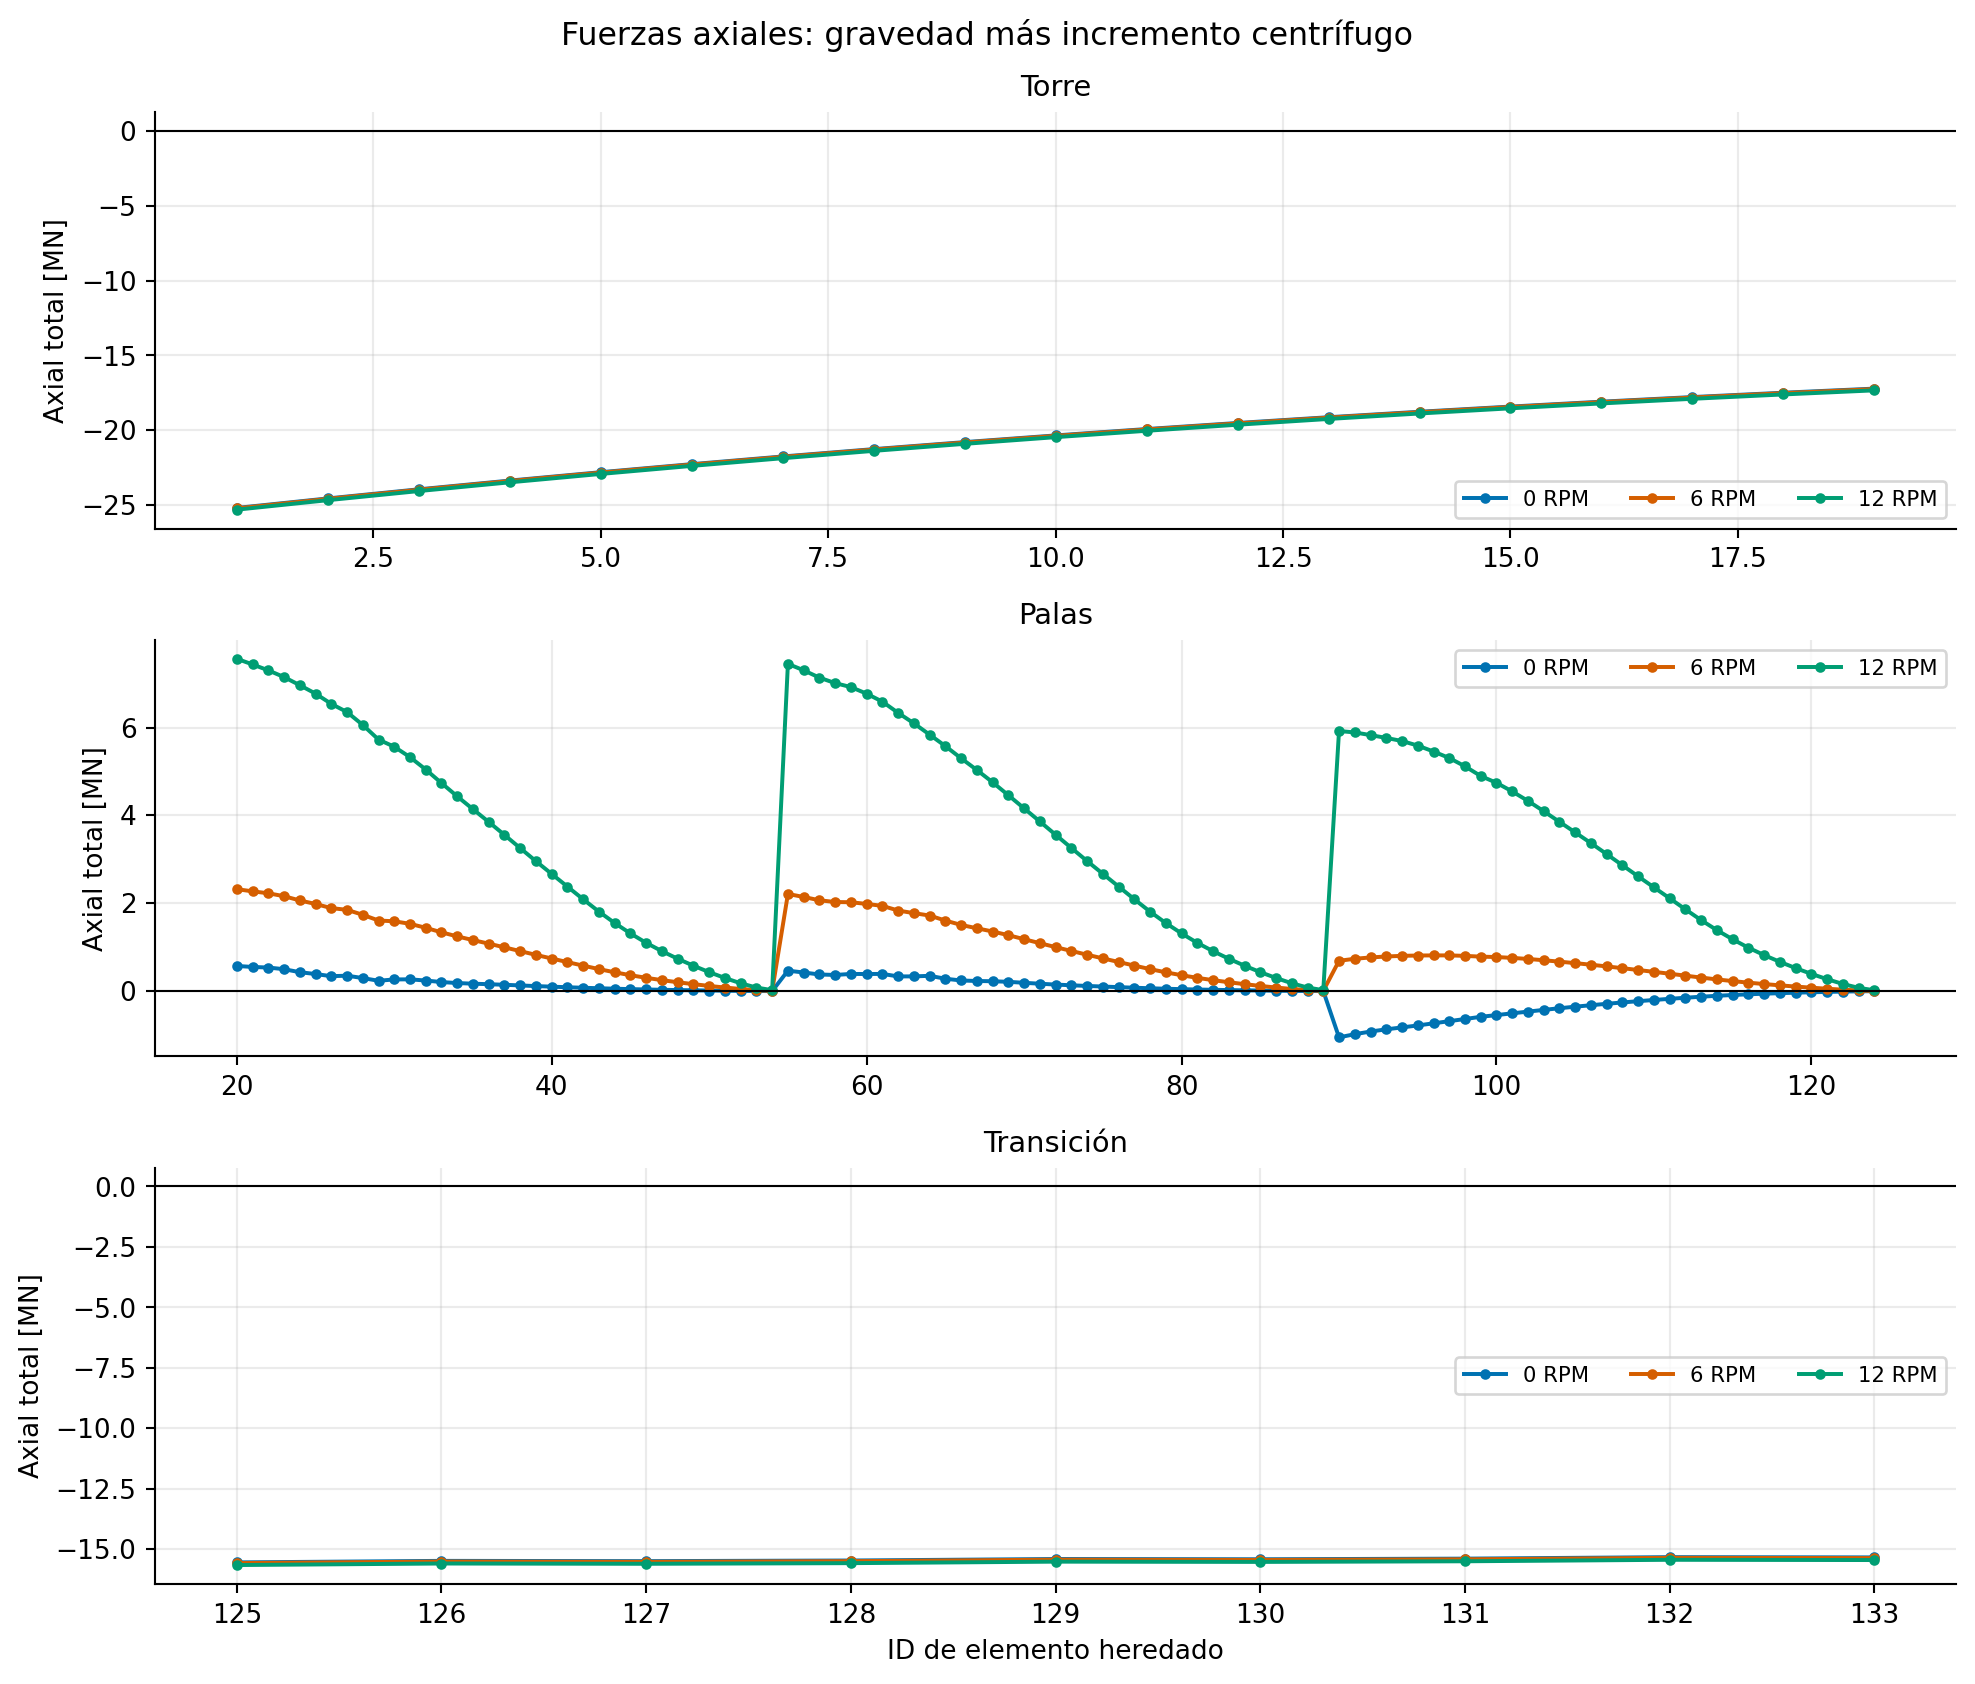
\includegraphics[width=\textwidth,height=0.69\textheight,keepaspectratio]{15_fuerzas_axiales_equilibrio.png}
\caption{Axiales totales por torre, palas y transiciones para 0, 6 y 12 RPM.}
\label{fig:resultado-origen-15}
\end{figure}

En los resultados actuales la contribución centrífuga a la tangente está incluida en $\bm K_g$; por esa convención $\bm K_\Omega=\bm0$ y no se suma una segunda vez. La velocidad del rotor es prescrita: no se obtiene de un balance entre torque aerodinámico y generador.

\section{Operadores dinámicos, amortiguamiento y aerodinámica}

\subsection{Giroscopía}

La giroscopía de cada pala se integra con la cinemática Timoshenko y el cubo aporta su matriz espacial. Torre, góndola y cimentación no rotan. El operador entra en la parte proporcional a velocidad de la ecuación linealizada,

\[
\bm M\ddot{\bm q}+(\bm C+\bm G)\dot{\bm q}+\bm K\bm q=\bm f(t),
\qquad
\bm G^T=-\bm G,
\qquad
\bm v^T\bm G\bm v=0.
\]

Así, $\bm G$ modifica las frecuencias y acopla direcciones, pero no disipa energía. A 12 RPM:

\begin{itemize}
\item \nolinkurl{||G_distribuida||_F = 1.718598e5};
\item \nolinkurl{||G_cubo||_F = 5.063984e6};
\item normas por pala: 99,209.622; 99,219.879; 99,240.373;
\item dispersión relativa entre palas: \texttt{3.0992e-4}\allowbreak{}.
\end{itemize}

La contribución del cubo es aproximadamente 29.5 veces la norma distribuida de las palas. El crecimiento lineal con $\Omega$ explica por qué el desdoblamiento modal aparece progresivamente en el Campbell, aun sin aplicar viento.

\begin{figure}[!htbp]
\centering
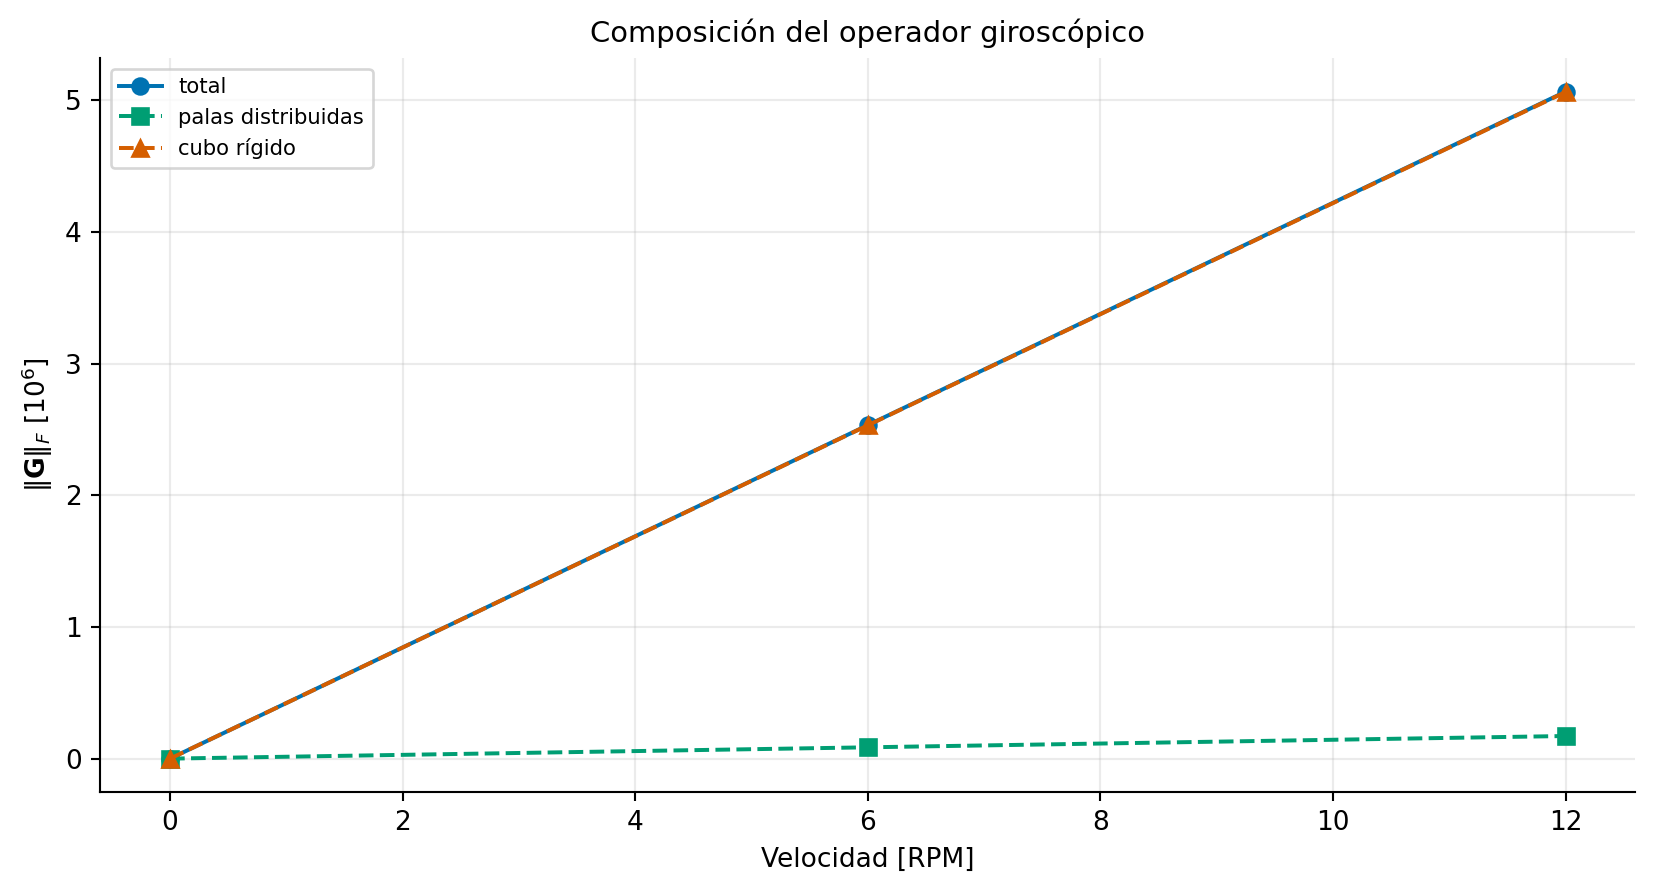
\includegraphics[width=\textwidth,height=0.69\textheight,keepaspectratio]{16_operador_giroscopico.png}
\caption{Crecimiento lineal y composición de la norma del operador giroscópico; el cubo rígido domina sobre la contribución distribuida.}
\label{fig:resultado-origen-16}
\end{figure}

\subsection{Amortiguamiento Rayleigh}

El modelo adopta 1\% de amortiguamiento en 0.2 y 2.0 Hz y obtiene

\[
\bm C_R=\alpha\bm M+\beta\bm K_e,
\qquad
\zeta(\omega)=\frac12\left(\frac{\alpha}{\omega}+\beta\omega\right),
\]

con $\alpha=0.02284794657\;\mathrm{s}^{-1}$ y $\beta=0.001446863119\;\mathrm{s}$. El valor esperado en ambos puntos de anclaje es $\zeta=0.01$ y el error absoluto calculado es $1.735\times10^{-18}$. La rigidez de referencia es $\bm K_e$, no la tangente operativa completa. El 1\% es un supuesto de cálculo y no procede de una identificación modal experimental.

\begin{figure}[!htbp]
\centering
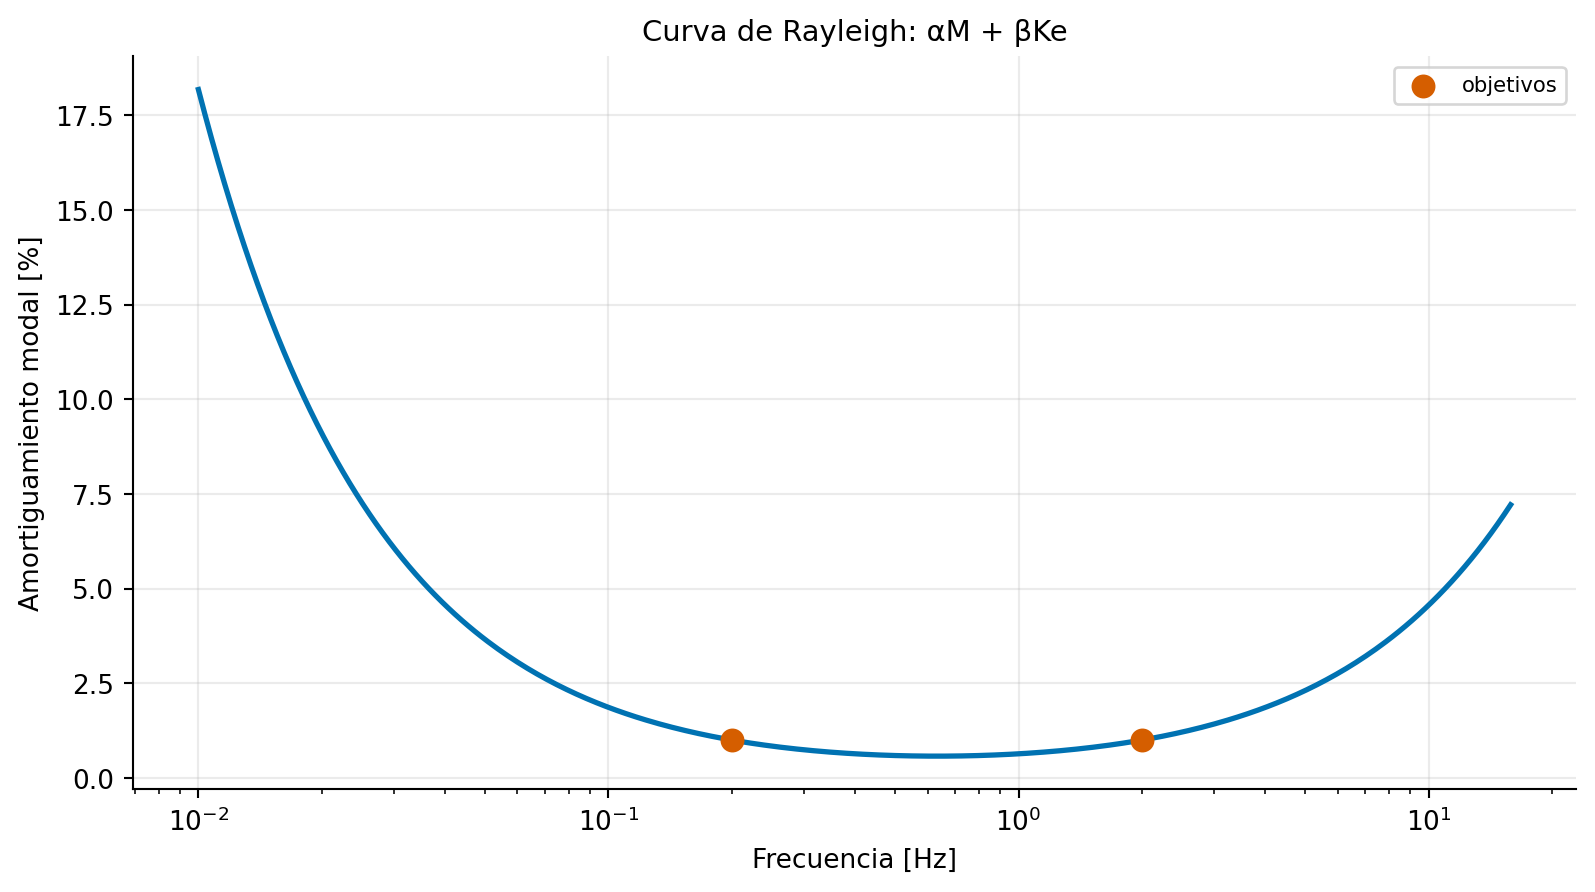
\includegraphics[width=\textwidth,height=0.69\textheight,keepaspectratio]{17_amortiguamiento_rayleigh.png}
\caption{La curva pasa por los dos valores adoptados de 1\%, pero fuera de ellos el amortiguamiento es una extrapolación del modelo de Rayleigh.}
\label{fig:resultado-origen-17}
\end{figure}

\subsection{Inserción de cargas de viento y alcance actual}

El solver admite una fuerza aerodinámica generalizada no lineal $\bm f_a(\bm q,\dot{\bm q},t)$, evaluada en el equilibrio junto con gravedad y centrifugación. Al linealizar alrededor del estado operativo $(\bm q_0,\dot{\bm q}_0)$ se definen

\[
\bm K_a=-\left.\frac{\partial\bm f_a}{\partial\bm q}\right|_0,
\qquad
\bm C_a=-\left.\frac{\partial\bm f_a}{\partial\dot{\bm q}}\right|_0,
\]

de forma que ambos operadores pasan al lado izquierdo:

\[
\bm D=\bm C_s+\bm C_a+\bm G,
\qquad
\bm K=\bm K_e+\bm K_g+\bm K_\Omega+\bm K_a.
\]

Si el modelo externo suministra tangentes analíticas se usan directamente. En caso contrario, cada columna se calcula por diferencias centrales,

\[
(\bm K_a)_{:,j}\simeq-
\frac{\bm f_a(\bm q_0+h_j\bm e_j,\dot{\bm q}_0)
-\bm f_a(\bm q_0-h_j\bm e_j,\dot{\bm q}_0)}{2h_j},
\]

con una expresión análoga para $\bm C_a$ perturbando la velocidad. La razón de errores entre pasos $h$ y $h/2$ fue 4.000, igual al valor esperado para una diferencia central de segundo orden; los errores relativos de las tangentes de referencia fueron $3.583\times10^{-8}$ y $3.397\times10^{-8}$.

Sin embargo, \textbf{en todos los resultados físicos de este informe} se tiene $\bm f_a=\bm0$, $\bm K_a=\bm0$ y $\bm C_a=\bm0$ porque no se proporcionaron coeficientes aerodinámicos. No hay velocidad o dirección de viento, densidad del aire, perfil vertical, turbulencia, ráfaga, polares, BEM, control de pitch o yaw, empuje ni torque aerodinámico. Por tanto, el equilibrio, Campbell y sismo presentados incluyen giro prescrito, gravedad y centrifugación, pero \textbf{no una carga de viento} ni combinación sismo--viento.

\section{MBC, problema cuadrático y Campbell}

\subsection{Transformación multiblade físicamente homóloga}

Antes de mezclar armónicos, cada pala se expresa en marcos locales homólogos. Si $\bm z$ contiene coordenadas colectivas, coseno y seno, la transformación dependiente del azimut es

\[
\bm q=\bm P(t)\bm z,
\qquad
\bm P=\bm H\bm T_B.
\]

Al derivar $\bm q$ aparecen $\dot{\bm P}$ y $\ddot{\bm P}$; por eso los operadores transformados no son una simple congruencia:

\[
\bar{\bm M}=\bm P^T\bm M\bm P,
\]

\[
\bar{\bm D}=\bm P^T
(\bm D\bm P+2\bm M\dot{\bm P}),
\]

\[
\bar{\bm K}=\bm P^T
(\bm K\bm P+\bm D\dot{\bm P}+\bm M\ddot{\bm P}).
\]

Las métricas se comparan con la precisión esperada de las operaciones y de las diferencias finitas: ortogonalidad de $\bm H$, $1.377\times10^{-16}$ frente a $10^{-12}$; identidad $\bm P^{-1}\bm P$, $7.160\times10^{-16}$ frente a $10^{-12}$; derivada primera, $4.811\times10^{-11}$ frente a $10^{-8}$; derivada segunda, $2.101\times10^{-6}$ frente a $2\times10^{-5}$; y reconstrucción, $2.781\times10^{-16}$ frente a $10^{-12}$. Estos errores son mucho menores que las variaciones modales interpretadas en el Campbell.

\subsection{QEP y equivalencia a velocidad cero}

En cada velocidad se linealiza alrededor del equilibrio y se resuelve el problema cuadrático de autovalores (QEP)

\[
\bm Q(s)\bm\phi
=\left(s^2\bm M+s\bm D+\bm K\right)\bm\phi=\bm0,
\qquad s=\sigma+\mathrm i\omega_d .
\]

No se forma $\bm M^{-1}$. El polinomio se convierte en el lápiz generalizado

\[
\begin{bmatrix}
\bm0&\bm I\\
-\bm K&-\bm D
\end{bmatrix}
\begin{bmatrix}\bm\phi\\s\bm\phi\end{bmatrix}
=s
\begin{bmatrix}
\bm I&\bm0\\
\bm0&\bm M
\end{bmatrix}
\begin{bmatrix}\bm\phi\\s\bm\phi\end{bmatrix}.
\]

Los 804 GDL producen un lápiz de orden 1608. El solucionador disperso extrae 28 raíces próximas al origen; se reporta un representante con parte imaginaria positiva de cada uno de los 12 pares físicos y cuatro raíces sirven de margen de selección. Para cada raíz,

\[
f_d=\frac{|\operatorname{Im}s|}{2\pi},
\qquad
f_n=\frac{|s|}{2\pi},
\qquad
\zeta=-\frac{\operatorname{Re}s}{|s|}.
\]

La distancia normalizada del par calculado a la ecuación original es

\[
\rho_i=
\frac{\|\bm Q(s_i)\bm\phi_i\|_2}
{\left(|s_i|^2\|\bm M\|_2+|s_i|\|\bm D\|_2+
\|\bm K\|_2\right)\|\bm\phi_i\|_2}.
\]

A 0 RPM, el problema conservativo y la formulación MBC coinciden con error relativo $3.452\times10^{-13}$; el valor esperado es menor que $10^{-6}$. Al anular el amortiguamiento, el QEP recupera las frecuencias conservativas con error $6.112\times10^{-13}$. El máximo $\rho_i$ fue $2.505\times10^{-16}$ frente al criterio $10^{-8}$; el residuo adjunto fue $7.494\times10^{-14}$, el error de pares conjugados fue cero y la parte fuera de diagonal biortogonal fue $7.602\times10^{-11}$ frente a $10^{-6}$.

\begin{figure}[!htbp]
\centering
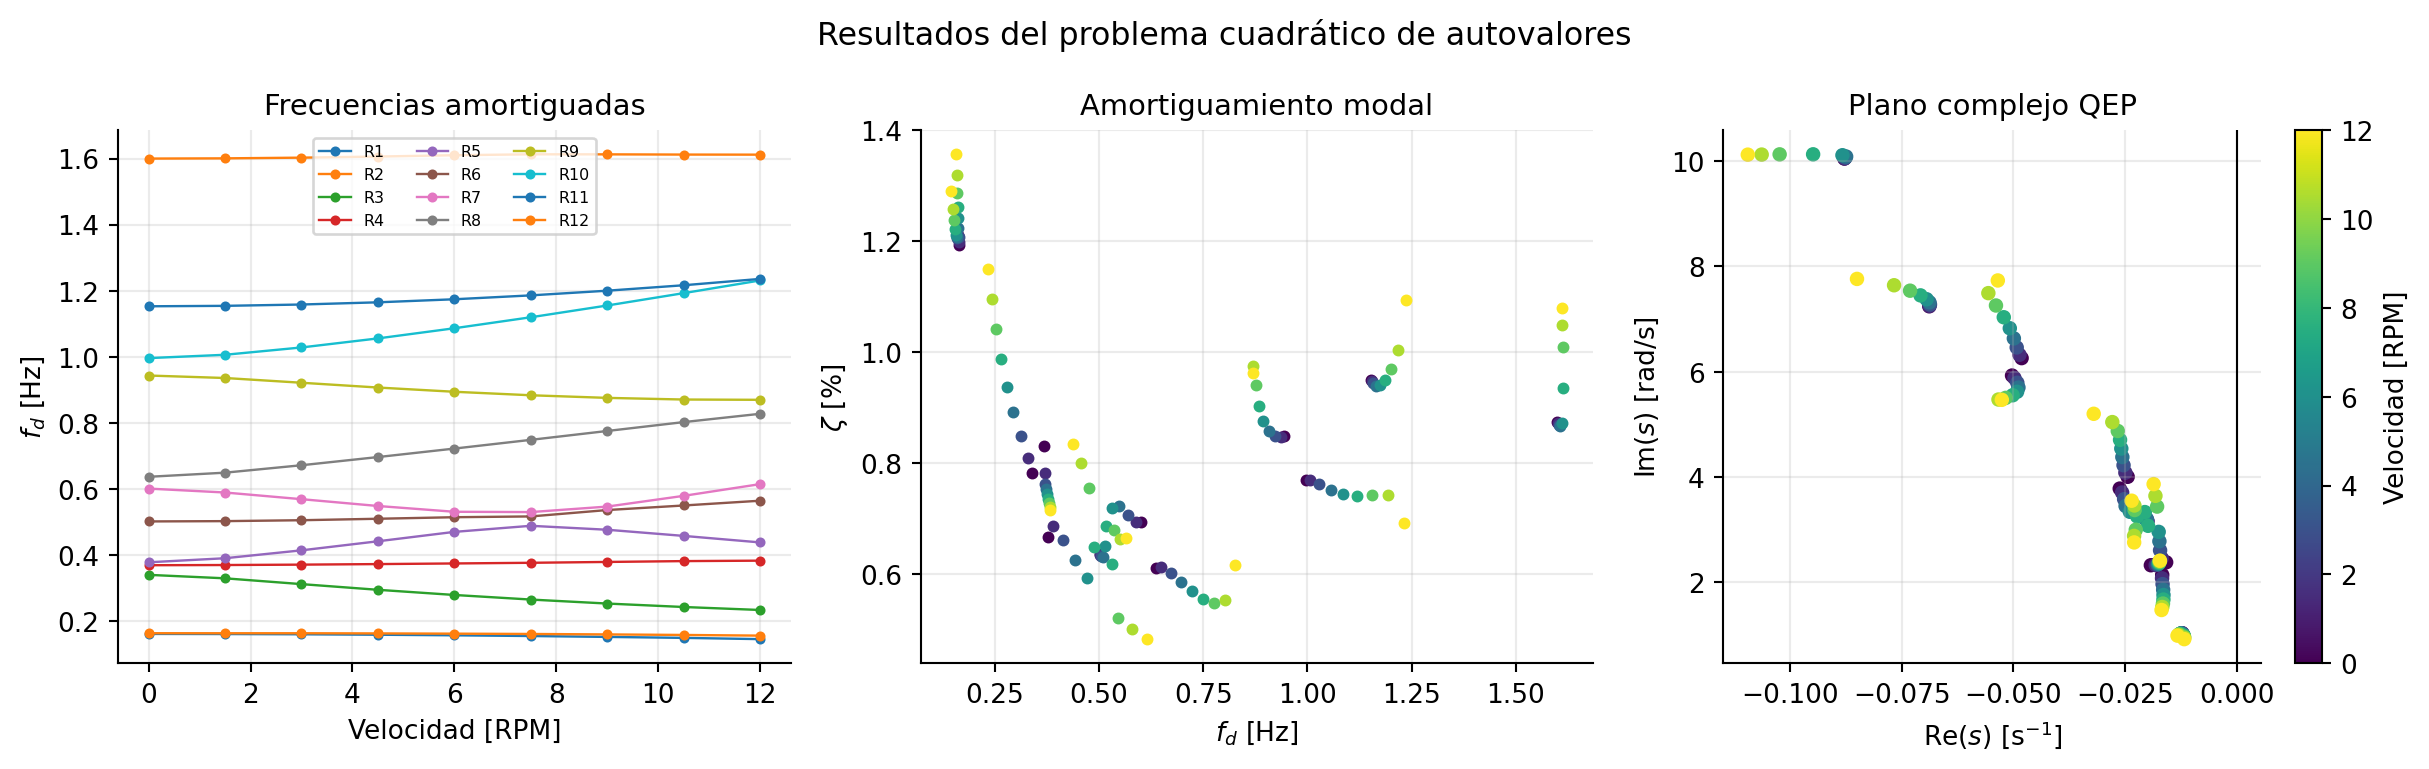
\includegraphics[width=\textwidth,height=0.69\textheight,keepaspectratio]{21_calidad_qep.png}
\caption{Frecuencias amortiguadas, razones de amortiguamiento y raíces del QEP en el plano complejo. La ubicación de cada raíz determina $f_d$ y $\zeta$.}
\label{fig:resultado-origen-21}
\end{figure}

La máxima parte real de las raíces extraídas fue $-1.181\times10^{-2}\;\mathrm{s}^{-1}$, correspondiente a la rama 1 a 12 RPM. Por tanto, ninguna de las 12 ramas calculadas crece exponencialmente. Esto no certifica la estabilidad del espectro completo, pues solo se extrajeron 28 de las 1608 raíces del lápiz.

\subsection{Diagrama Campbell y seguimiento}

El Campbell usa nueve velocidades entre 0 y 12 RPM y sigue 12 ramas. Dos modos en velocidades consecutivas se asocian mediante

\[
\operatorname{MAC}_{ij}
=\frac{|\bm\phi_i^H\bm M\bm\phi_j|^2}
{(\bm\phi_i^H\bm M\bm\phi_i)
(\bm\phi_j^H\bm M\bm\phi_j)}.
\]

Fuera de dobletes casi degenerados, el MAC mínimo fue 0.8289 frente al valor esperado 0.80. En los dobletes se comparan subespacios mediante ángulos principales; el mínimo fue 0.9693 frente a 0.95. Esta distinción evita interpretar como pérdida de continuidad una rotación arbitraria de la base dentro del mismo subespacio modal.

\begin{figure}[!htbp]
\centering
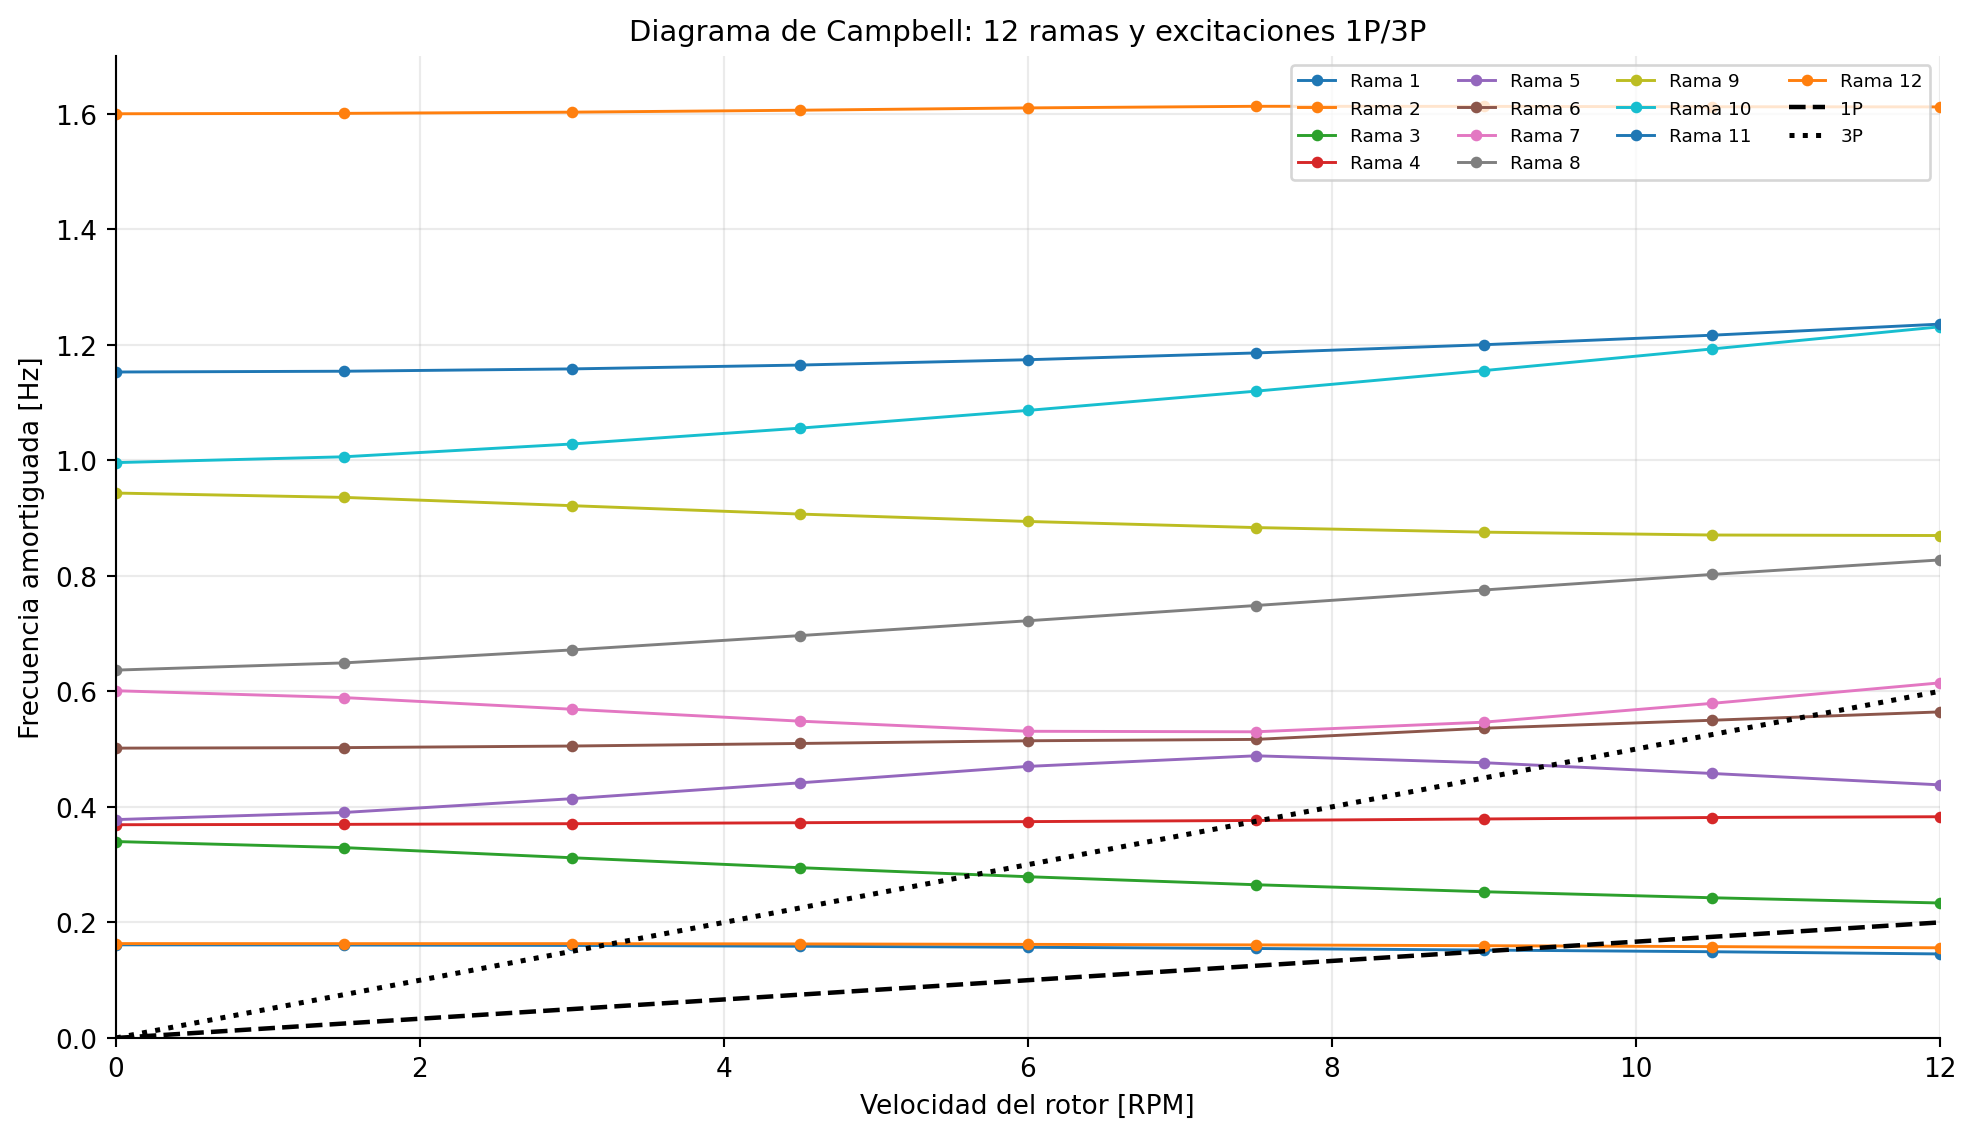
\includegraphics[width=\textwidth,height=0.69\textheight,keepaspectratio]{19_diagrama_campbell.png}
\caption{Doce ramas sobre nueve velocidades; las rectas 1P y 3P representan las frecuencias de paso del rotor y de tres palas.}
\label{fig:resultado-origen-19}
\end{figure}

Las frecuencias de excitación cinemática son

\[
f_{1P}=\frac{\mathrm{RPM}}{60},
\qquad
f_{3P}=3\,\frac{\mathrm{RPM}}{60}.
\]

A 0 RPM, las 12 ramas cubren de 0.161234 a 1.599818 Hz. A 12 RPM las frecuencias amortiguadas son:

\[
\begin{aligned}
\bm f_d(12\ \mathrm{RPM})={}&
\{0.145471,\ 0.156113,\ 0.233688,\ 0.382958,\ 0.438185,\ 0.564397,\\
&0.614622,\ 0.827431,\ 0.869749,\ 1.230962,\ 1.235641,\ 1.611690\}
\ \mathrm{Hz}.
\end{aligned}
\]

La razón de amortiguamiento calculada en el barrido varía entre 0.483\% y 1.357\%. La interpolación lineal identifica coincidencias 1P con las ramas 1 y 2 a 9.119 y 9.549 RPM, y coincidencias 3P con las ramas 1--6 a 3.200, 3.264, 5.655, 7.532, 9.425 y 11.118 RPM. Son \textbf{candidatos de resonancia}, no resonancias críticas: faltan las amplitudes de excitación, el viento, el control y un criterio de margen.

El Campbell está congelado en un azimut de referencia. No es un análisis de Floquet ni reproduce por sí solo la periodicidad completa de una turbina en rotación.

\subsection{Formas modales recuperadas}

Las seis formas siguientes son las primeras ramas exportadas del caso integral. La deformación está amplificada para hacer visible el patrón; no representa una amplitud física.

\begin{figure}[!htbp]
\centering
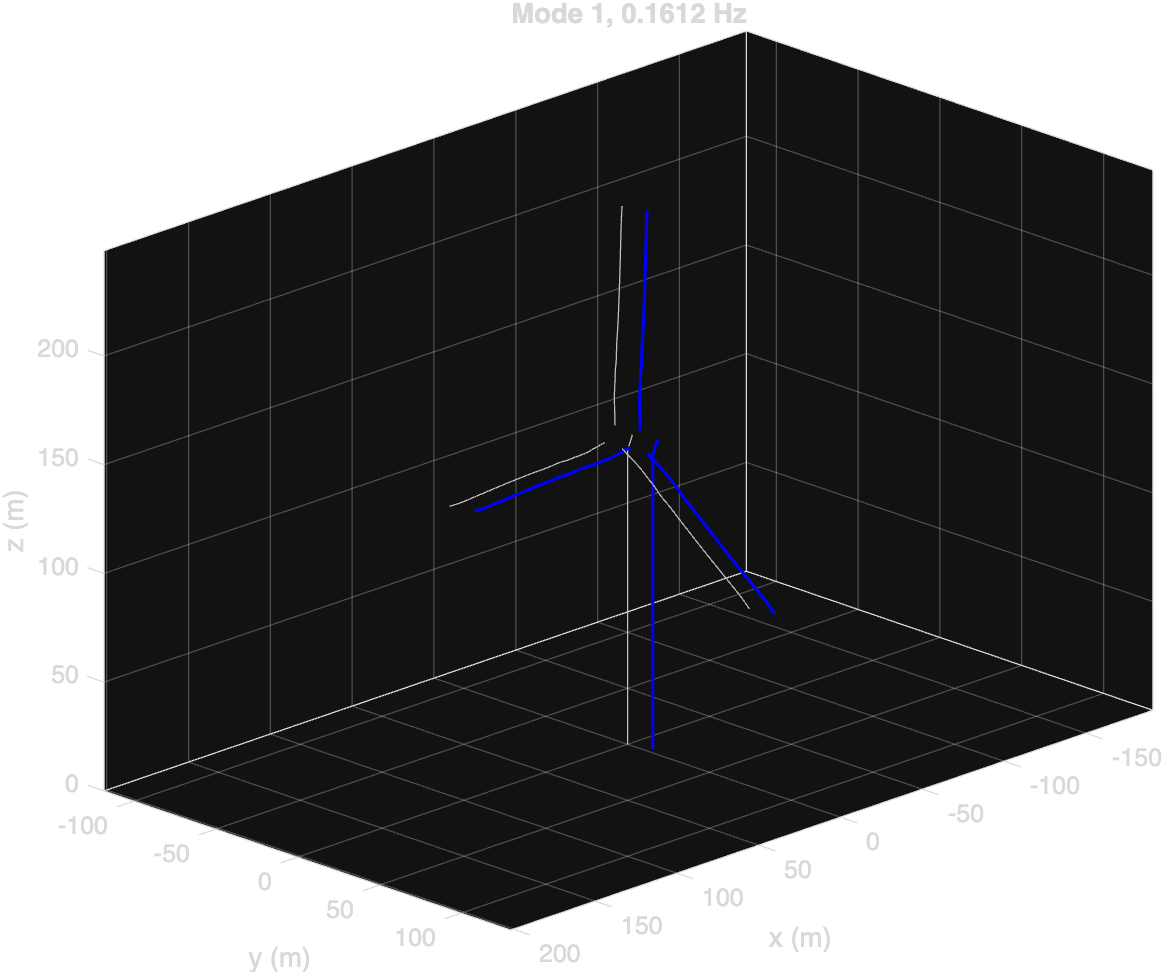
\includegraphics[width=\textwidth,height=0.69\textheight,keepaspectratio]{34_forma_modal_01.png}
\caption{Forma modal 1 a 0 RPM: primera rama del tren de potencia, 0.161234 Hz. La amplitud se normaliza y amplifica solo para visualización.}
\label{fig:resultado-origen-34}
\end{figure}

\begin{figure}[!htbp]
\centering
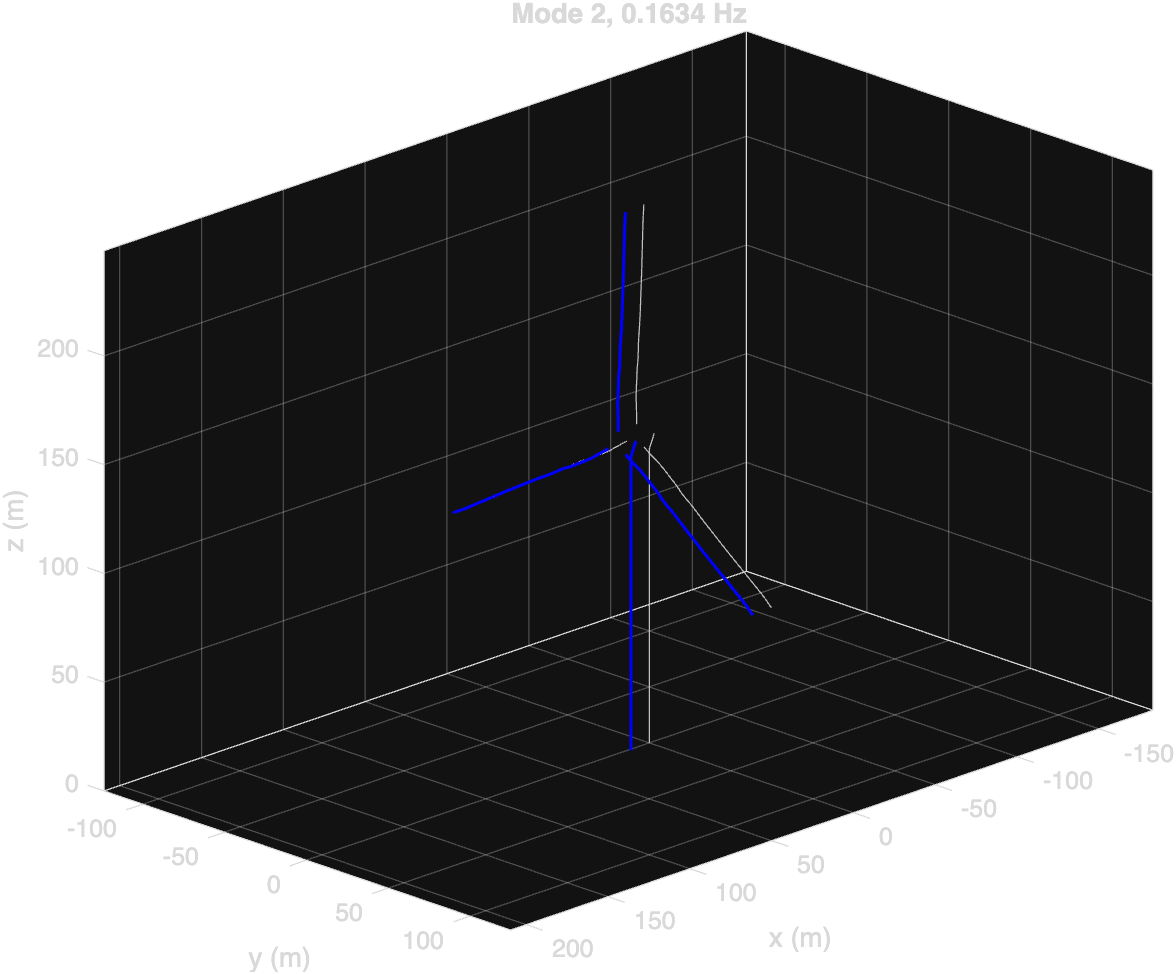
\includegraphics[width=\textwidth,height=0.69\textheight,keepaspectratio]{35_forma_modal_02.png}
\caption{Forma modal 2 a 0 RPM: segunda rama del tren de potencia, 0.163378 Hz. La amplitud mostrada no es una respuesta física.}
\label{fig:resultado-origen-35}
\end{figure}

\begin{figure}[!htbp]
\centering
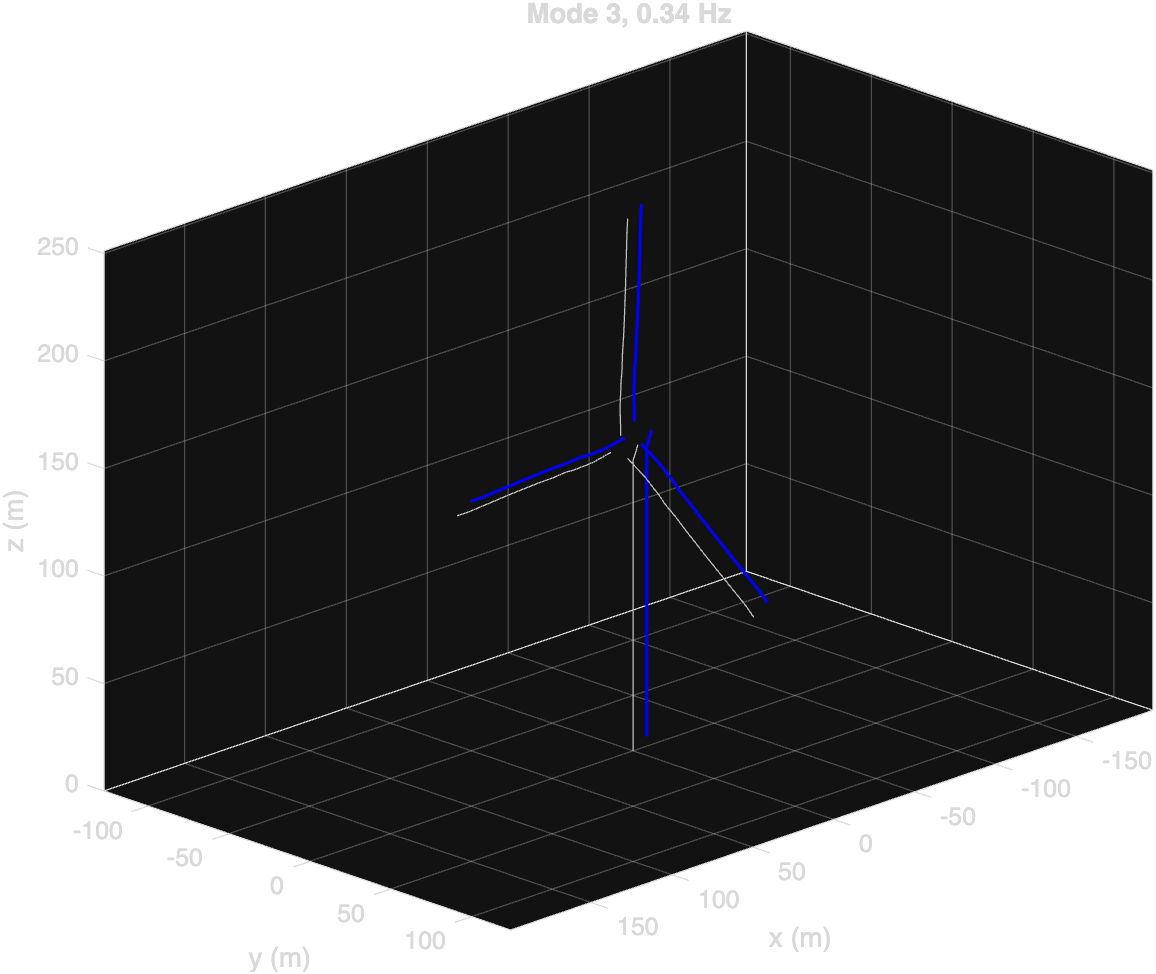
\includegraphics[width=\textwidth,height=0.69\textheight,keepaspectratio]{36_forma_modal_03.png}
\caption{Forma modal 3 a 0 RPM: rama dominada por palas, 0.340023 Hz.}
\label{fig:resultado-origen-36}
\end{figure}

\begin{figure}[!htbp]
\centering
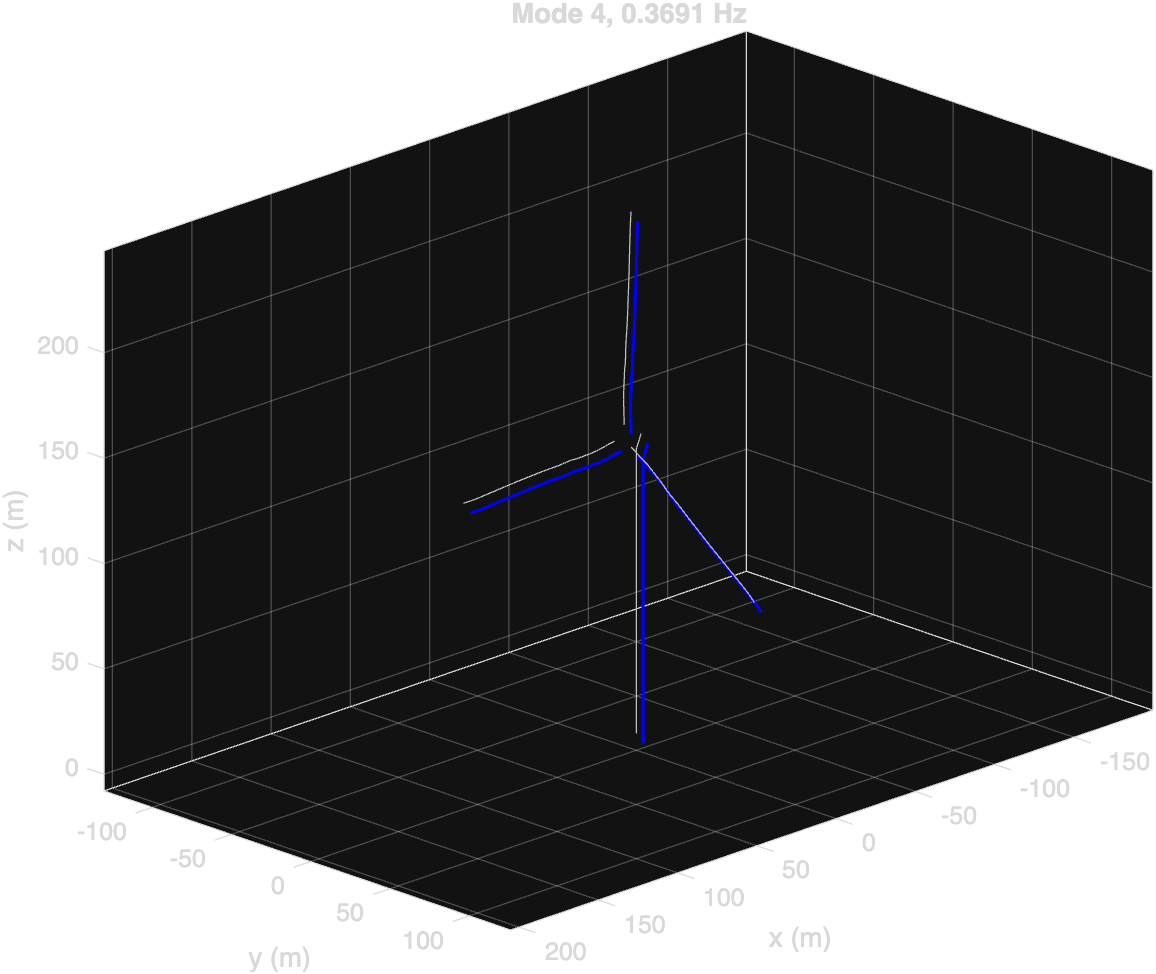
\includegraphics[width=\textwidth,height=0.69\textheight,keepaspectratio]{37_forma_modal_04.png}
\caption{Forma modal 4 a 0 RPM: rama dominada por palas, 0.369133 Hz.}
\label{fig:resultado-origen-37}
\end{figure}

\begin{figure}[!htbp]
\centering
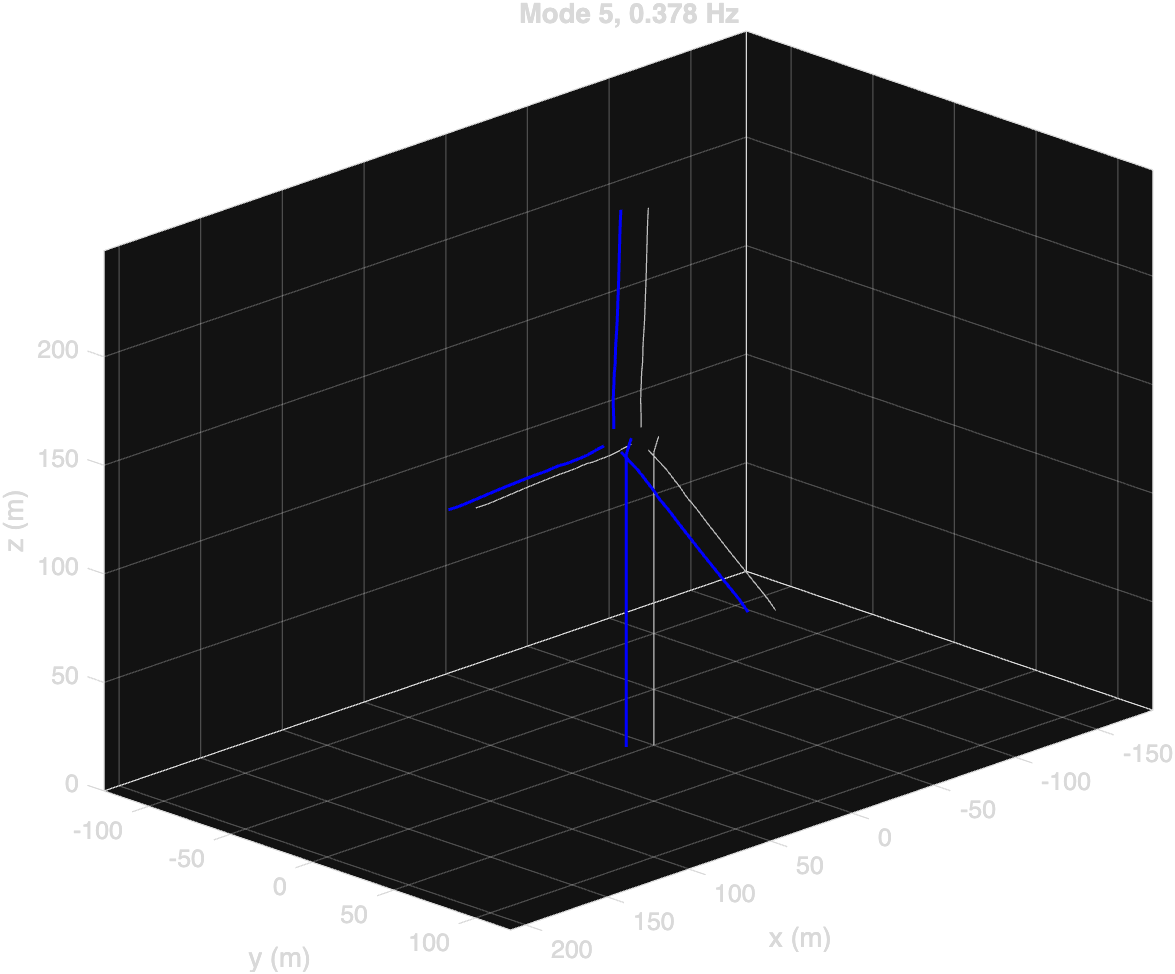
\includegraphics[width=\textwidth,height=0.69\textheight,keepaspectratio]{38_forma_modal_05.png}
\caption{Forma modal 5 a 0 RPM: rama dominada por palas, 0.378025 Hz.}
\label{fig:resultado-origen-38}
\end{figure}

\begin{figure}[!htbp]
\centering
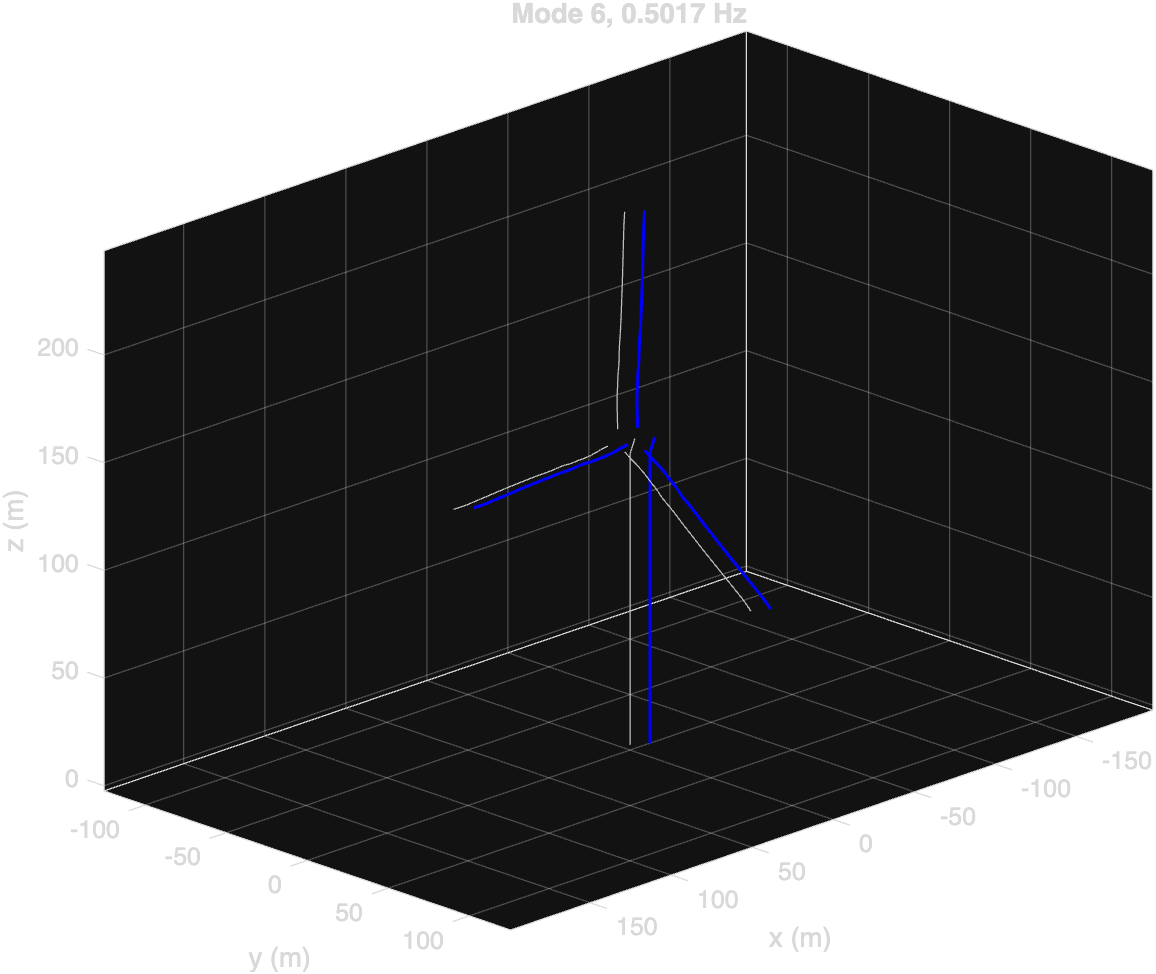
\includegraphics[width=\textwidth,height=0.69\textheight,keepaspectratio]{39_forma_modal_06.png}
\caption{Forma modal 6 a 0 RPM: rama dominada por palas, 0.501694 Hz.}
\label{fig:resultado-origen-39}
\end{figure}

\section{Respuesta sísmica con Newmark}

\subsection{Ecuación, entrada y proyección}

La coordenada $\bm q(t)$ describe movimiento \textbf{relativo al terreno}. Los operadores físicos se congelan en el equilibrio de 0 o 12 RPM y se resuelve

\[
\bm M_r\ddot{\bm q}
+\bm D_r\dot{\bm q}
+\bm K_r\bm q
=-\bm M_r\bm\Gamma_{\mathrm{eff}}\bm a_g(t)
+\bm f_{\mathrm{other}}(t),
\]

donde

\[
\bm M_r=\bm T_c^T\bm M_{\mathrm{full}}\bm T_c,
\qquad
\bm M_r\bm\Gamma_{\mathrm{eff}}
=\bm T_c^T\bm M_{\mathrm{full}}\bm R_{\mathrm{full}}.
\]

$\bm R_{\mathrm{full}}$ coloca una unidad en los GDL traslacionales de todos los nodos para cada dirección excitada. Al proyectar con masa aparece $\bm\Gamma_{\mathrm{eff}}$, que genera la fuerza inercial correcta incluso cuando las MPC ligan raíces y cubo. La influencia cinemática $\bm\Gamma_{\mathrm{kin}}$ se usa únicamente para reconstruir movimiento absoluto compatible:

\[
\bm u_{\mathrm{abs}}
=\bm T_c\bm q+\bm R_{\mathrm{full}}\bm u_g,
\quad
\bm v_{\mathrm{abs}}
=\bm T_c\dot{\bm q}+\bm R_{\mathrm{full}}\bm v_g,
\quad
\bm a_{\mathrm{abs}}
=\bm T_c\ddot{\bm q}+\bm R_{\mathrm{full}}\bm a_g.
\]

El lector de acelerogramas acepta arreglos, tablas, estructuras o archivos; convierte las unidades a SI, interpola al paso solicitado y, si faltan $\bm v_g$ o $\bm u_g$, las integra. También permite escala y corrección de línea base. Para estos resultados se suministraron directamente desplazamiento, velocidad y aceleración analíticos, con escala uno y sin corrección de línea base.

El movimiento sintético se aplica en las direcciones globales $x$ y $y$:

\[
u_{gx}(t)=0.003\sin^3(2\pi\,0.65\,t),\qquad
u_{gy}(t)=0.0018\sin^3(2\pi\,0.90\,t),
\qquad 0\leq t\leq1\ \mathrm{s},
\]

con $\bm v_g=\dot{\bm u}_g$ y $\bm a_g=\ddot{\bm u}_g$. Los máximos de desplazamiento son 3.0 y 1.8 mm; los de velocidad, aproximadamente 0.01415 y 0.01175 m/s; y las PGA, 0.1501 y 0.1727 m/s$^2$ (0.0153 y 0.0176 g). El estado inicial es nulo, pero el registro de un segundo no termina con todas sus derivadas en cero ni incluye una cola de vibración libre. Por ello sirve para comparar la respuesta de los dos puntos operativos, no como acelerograma de diseño.

\begin{figure}[!htbp]
\centering
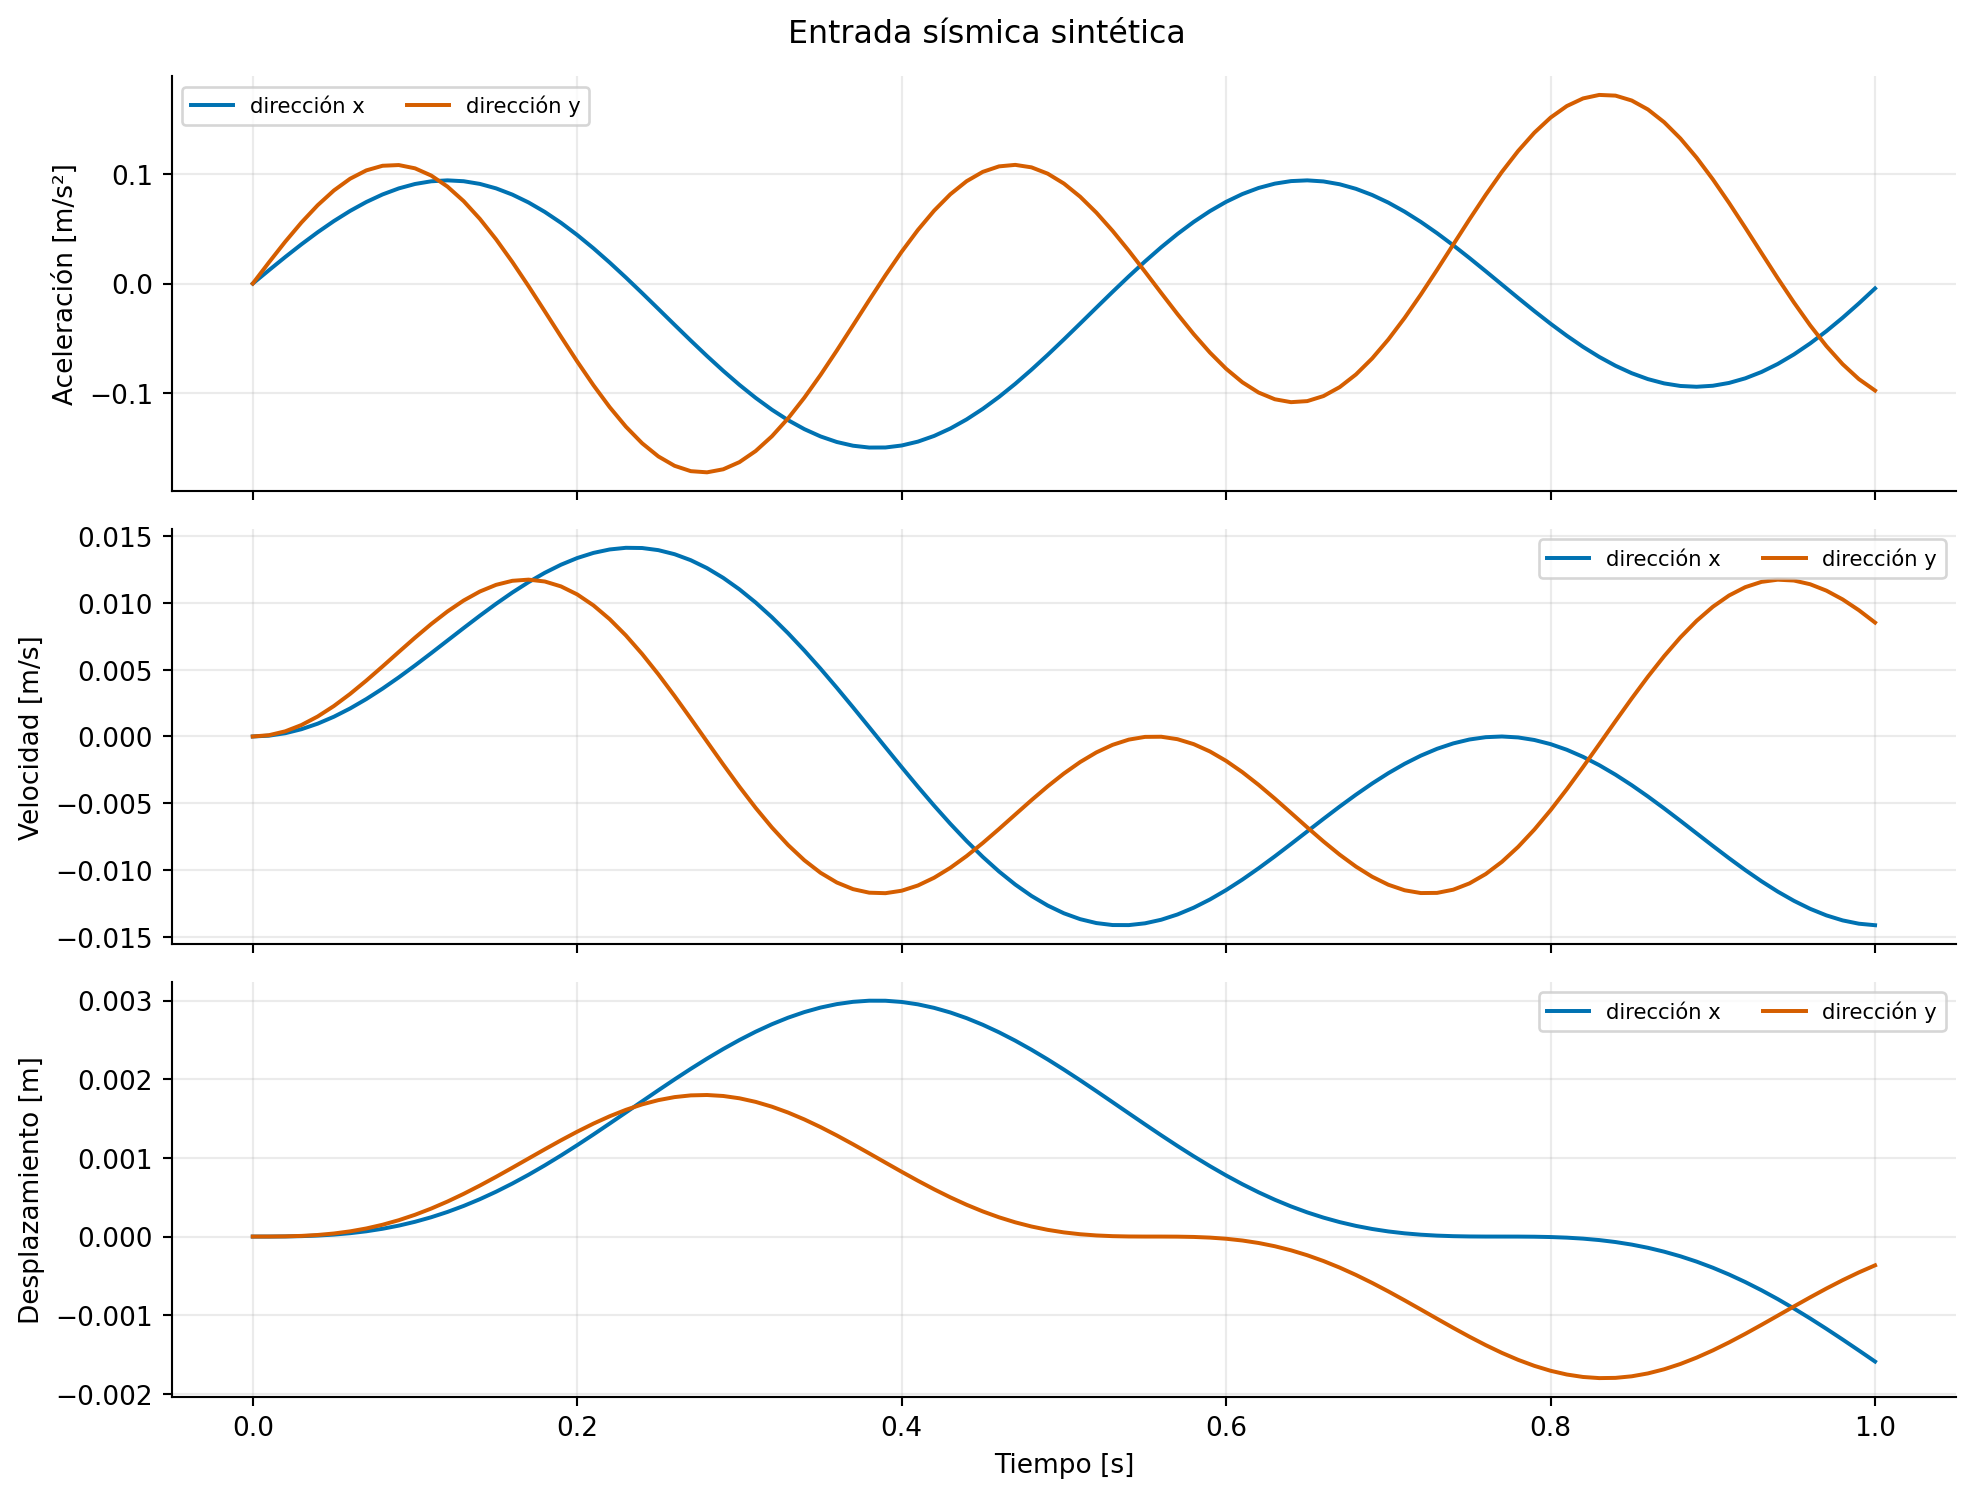
\includegraphics[width=\textwidth,height=0.69\textheight,keepaspectratio]{23_movimiento_sismico_entrada.png}
\caption{Entrada sísmica sintética en las direcciones globales x e y: aceleración, velocidad y desplazamiento del terreno en SI.}
\label{fig:resultado-origen-23}
\end{figure}

\subsection{Integración y convergencia temporal}

Se utilizó Newmark de aceleración promedio constante, $\beta=1/4$ y $\gamma=1/2$. Para un paso $\Delta t$ se definen

\[
a_0=\frac{1}{\beta\Delta t^2},
\qquad
a_1=\frac{\gamma}{\beta\Delta t},
\qquad
\bm K_{\mathrm{eff}}
=\bm K_r+a_0\bm M_r+a_1\bm D_r .
\]

En cada instante se construye una carga efectiva con la fuerza sísmica y los estados del paso anterior, se factoriza $\bm K_{\mathrm{eff}}$ y se obtiene $\bm q_{n+1}$ mediante solución lineal, sin invertir matrices. Luego,

\[
\ddot{\bm q}_{n+1}
=a_0(\bm q_{n+1}-\bm q_n)
-\frac{1}{\beta\Delta t}\dot{\bm q}_n
-\left(\frac{1}{2\beta}-1\right)\ddot{\bm q}_n,
\]

\[
\dot{\bm q}_{n+1}
=\dot{\bm q}_n+\Delta t
\left[(1-\gamma)\ddot{\bm q}_n+\gamma\ddot{\bm q}_{n+1}\right].
\]

El esquema es de segundo orden para el problema lineal. Un oscilador de un GDL dio error relativo fino $2.1861\times10^{-6}$ frente al valor esperado $10^{-4}$ y orden 1.9975 frente al esperado mínimo 1.9. En el modelo completo se usaron $\Delta t=\{0.02,0.01,0.005,0.0025,0.00125\}$ s: el orden observado fue 2.0017 frente al mínimo 1.8; la diferencia relativa entre las dos soluciones más finas fue $3.0719\times10^{-4}$ frente a $10^{-3}$, y la diferencia de máximos fue $2.3236\times10^{-4}$. La respuesta publicada usa $\Delta t=0.01$ s.

\begin{figure}[!htbp]
\centering
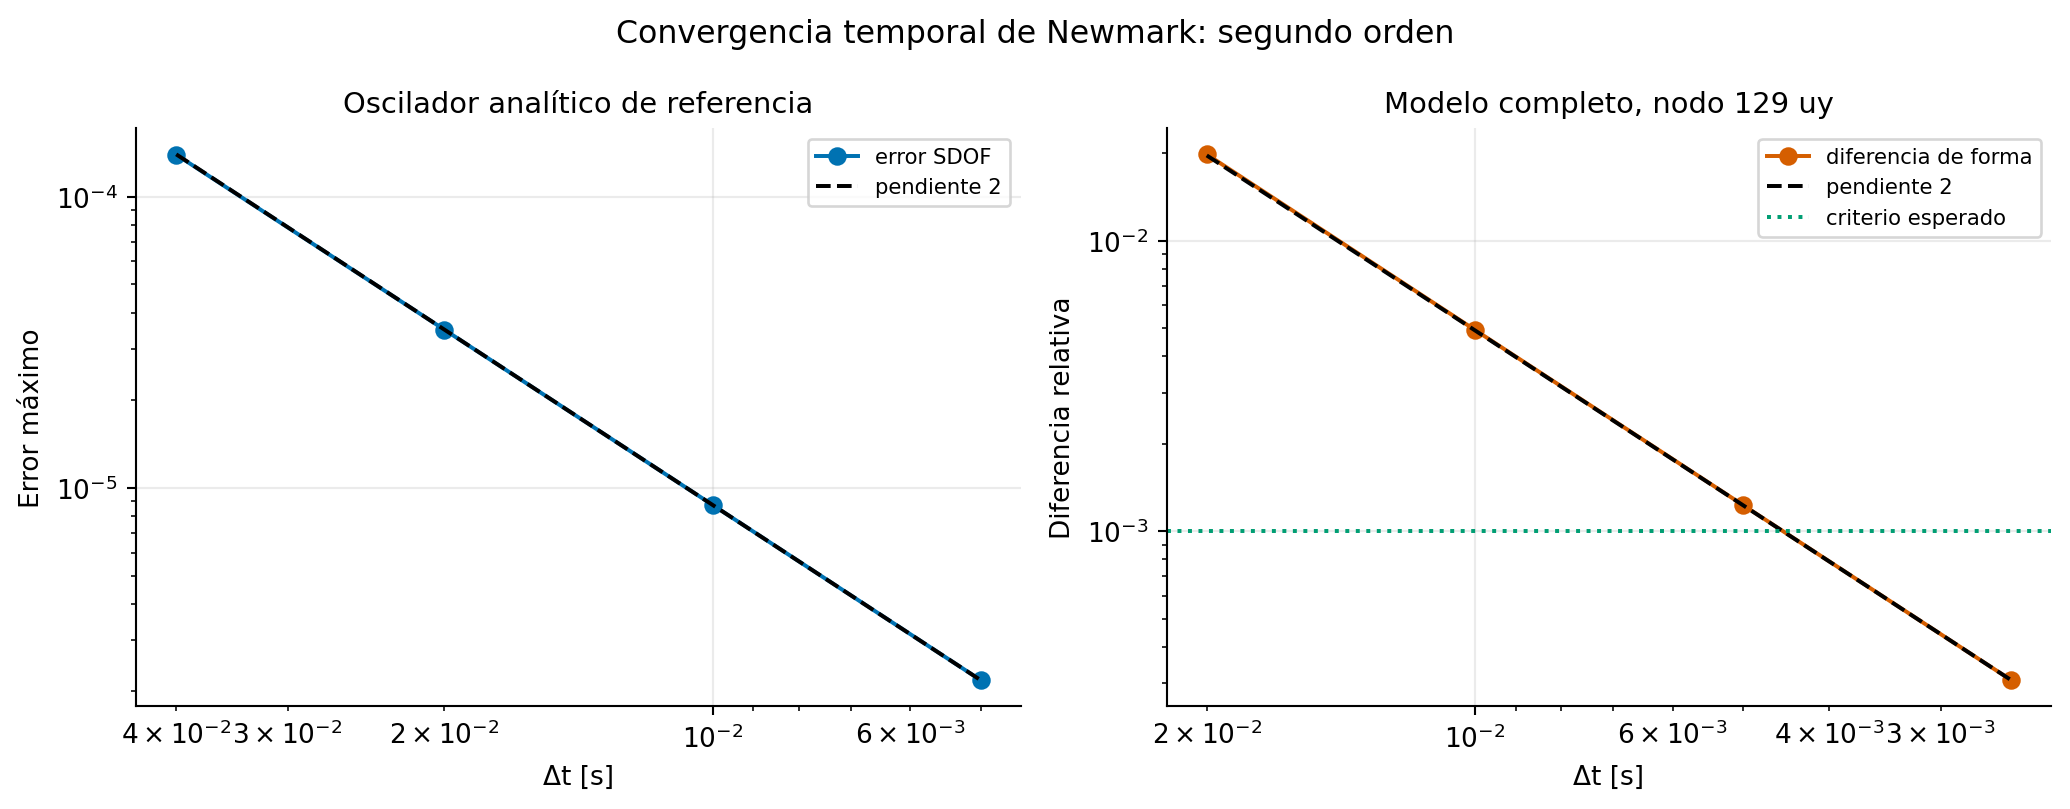
\includegraphics[width=\textwidth,height=0.69\textheight,keepaspectratio]{26_convergencia_temporal_newmark.png}
\caption{Convergencia temporal: la pendiente próxima a dos confirma el orden esperado de Newmark en el oscilador de referencia y en el canal nodo 129--uy.}
\label{fig:resultado-origen-26}
\end{figure}

\subsection{Respuesta, reacciones y fuerzas internas}

Se observan el nodo 1 en la base, el nodo 129 en la góndola, el nodo 130 en el rotor y los nodos 56, 92 y 128 en las puntas de las tres palas. Los ejes $x,y,z$ son los globales mostrados en la geometría. Antes de interpretar las amplitudes, las métricas numéricas se comparan con sus valores esperados:

\begingroup
\small
\renewcommand{\arraystretch}{1.16}
\begin{center}
\begin{tabularx}{\textwidth}{@{}YYYY@{}}
\toprule
\textbf{Métrica} & \textbf{Resultado} & \textbf{Valor esperado} & \textbf{Interpretación} \\
\midrule
Proyección de masa del sismo & \texttt{3.8771e-17}\allowbreak{} & $\leq10^{-12}$ & la fuerza reducida representa el campo completo \\
Residuo dinámico máximo & \texttt{6.1205e-13}\allowbreak{} & $\leq10^{-9}$ & cierre de la ecuación semidiscreta \\
Balance energético relativo & \texttt{1.0584e-12}\allowbreak{} & $\leq10^{-6}$ & trabajo de entrada y energía del sistema \\
Cinemática absoluta & \texttt{4.4345e-17}\allowbreak{} & $\leq10^{-12}$ & suma coherente de respuesta relativa y terreno \\
Equilibrio proyectado de restricciones & \texttt{6.2262e-13}\allowbreak{} & $\leq10^{-9}$ & compatibilidad entre fuerzas completas y reducidas \\
\bottomrule
\end{tabularx}
\end{center}
\endgroup

Estas tolerancias califican el error del procedimiento numérico; no son límites de servicio ni de resistencia de la turbina.

En el canal $u_y$ de la punta de pala del nodo 128 se obtuvo un desplazamiento relativo máximo absoluto de 15.167 mm a 0 RPM y 12.849 mm a 12 RPM; las aceleraciones absolutas máximas correspondientes fueron 1.816 y 1.687 m/s$^2$. Esto equivale a reducciones de 15.28\% y 7.10\% en ese canal. El máximo de aceleración entre todos los nodos observados del caso a 12 RPM fue 1.739 m/s$^2$, en el nodo 92 y dirección $x$. El cambio muestra que la rotación y el estado de equilibrio modifican la respuesta del caso sintético, pero no constituye por sí solo un factor de diseño.

\begin{figure}[!htbp]
\centering
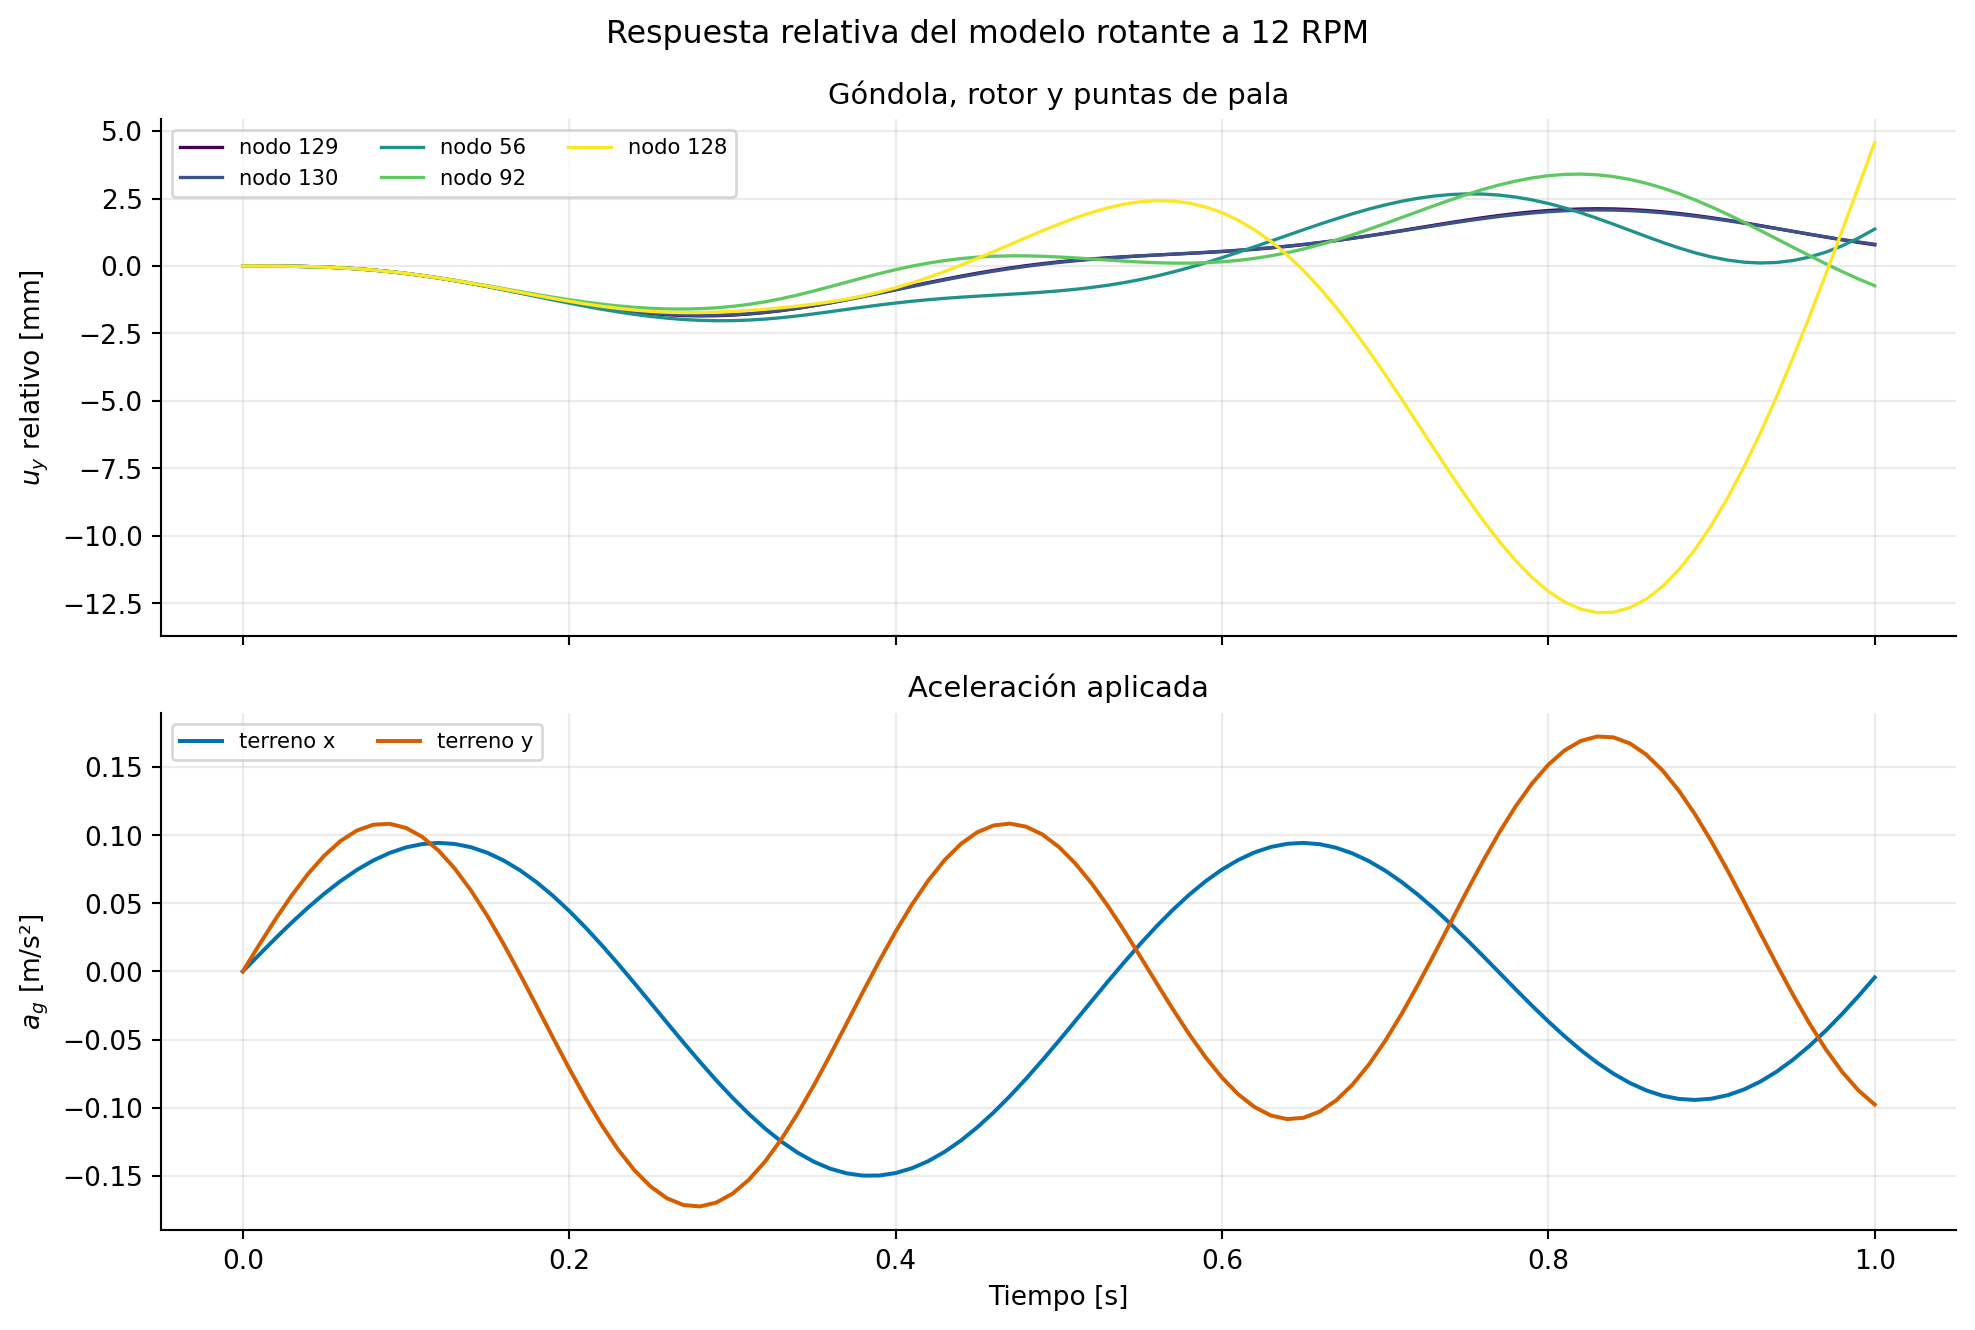
\includegraphics[width=\textwidth,height=0.69\textheight,keepaspectratio]{24_respuesta_sismica.png}
\caption{Respuesta relativa de góndola, rotor y puntas a 12 RPM, junto con la aceleración de terreno aplicada en x e y.}
\label{fig:resultado-origen-24}
\end{figure}

\begin{figure}[!htbp]
\centering
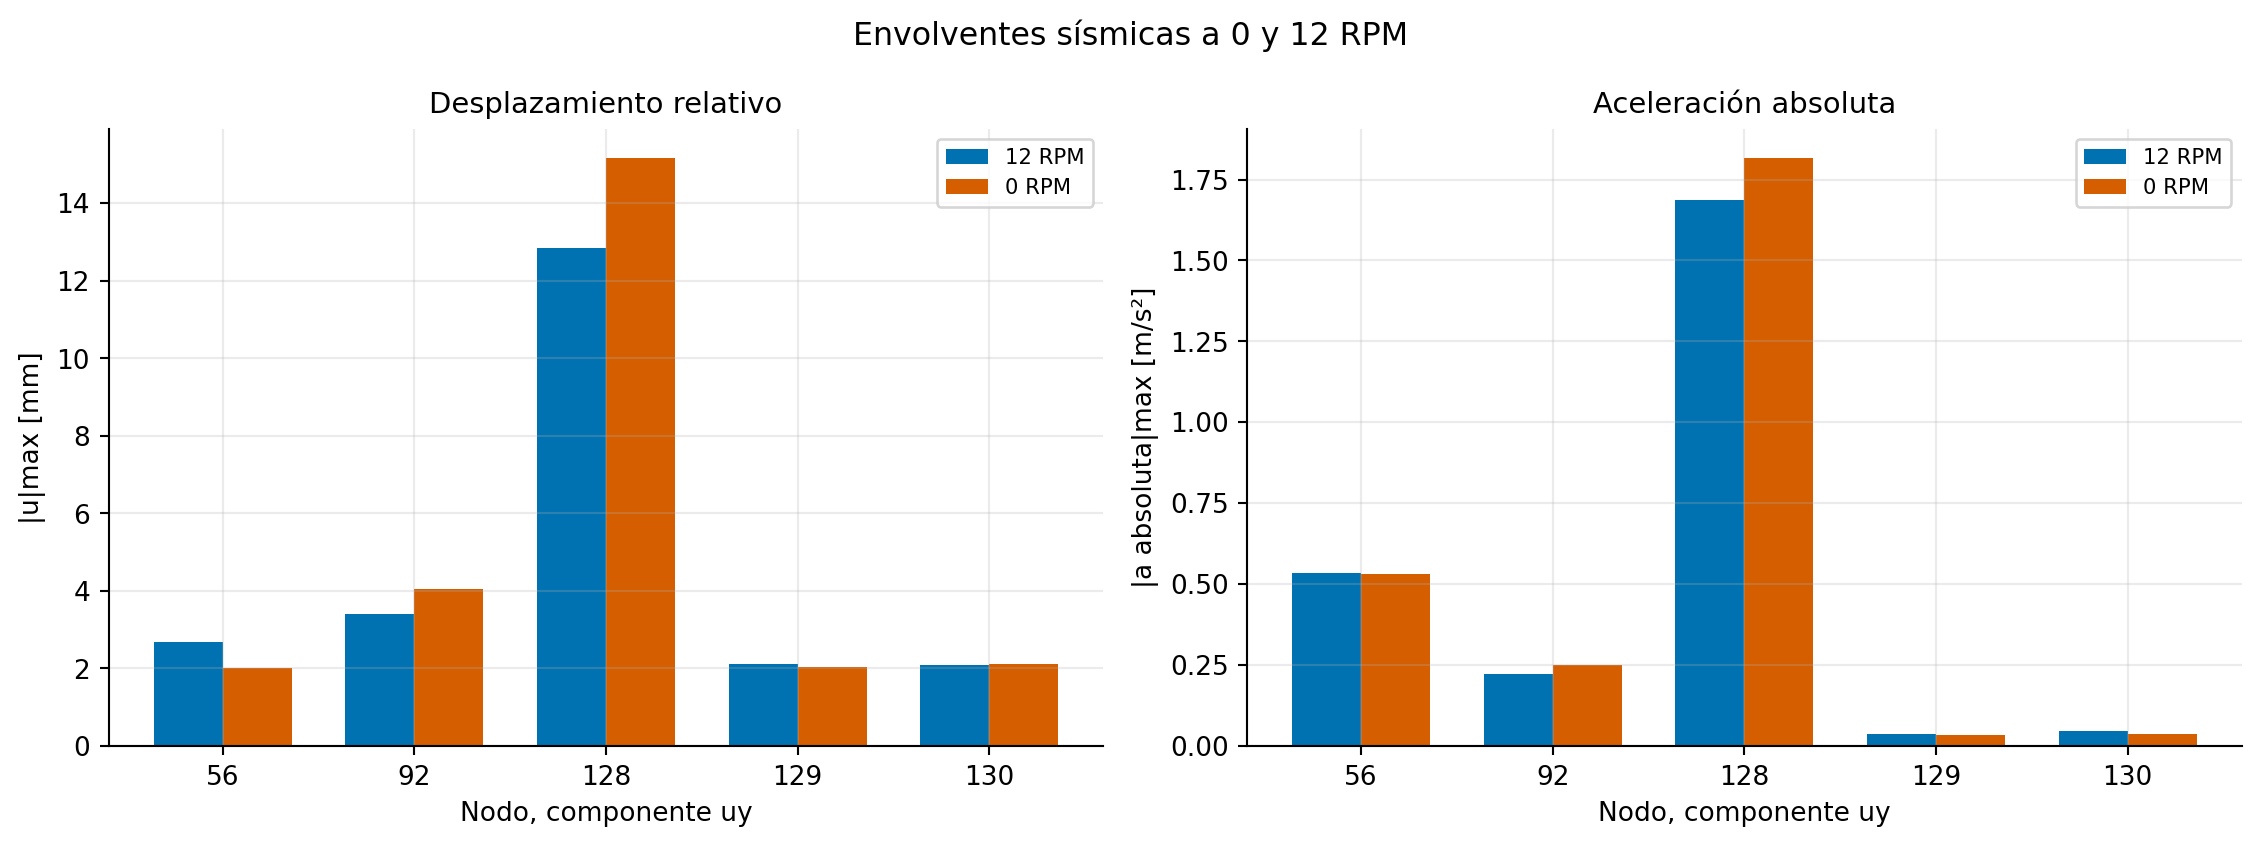
\includegraphics[width=\textwidth,height=0.69\textheight,keepaspectratio]{25_extremos_respuesta_sismica.png}
\caption{Envolventes uy y aceleración absoluta de nodos instrumentados.}
\label{fig:resultado-origen-25}
\end{figure}

En el caso rotante de 12 RPM, las reacciones máximas del nodo 1 fueron 91.035, 77.183 y 53.671 kN en $F_x,F_y,F_z$, y 3.520, 4.314 y 0.0418 MN\,$\cdot$\,m en $M_x,M_y,M_z$. Son incrementos debidos al movimiento sísmico alrededor del equilibrio operativo y no incluyen una comparación con capacidad resistente.

\begin{figure}[!htbp]
\centering
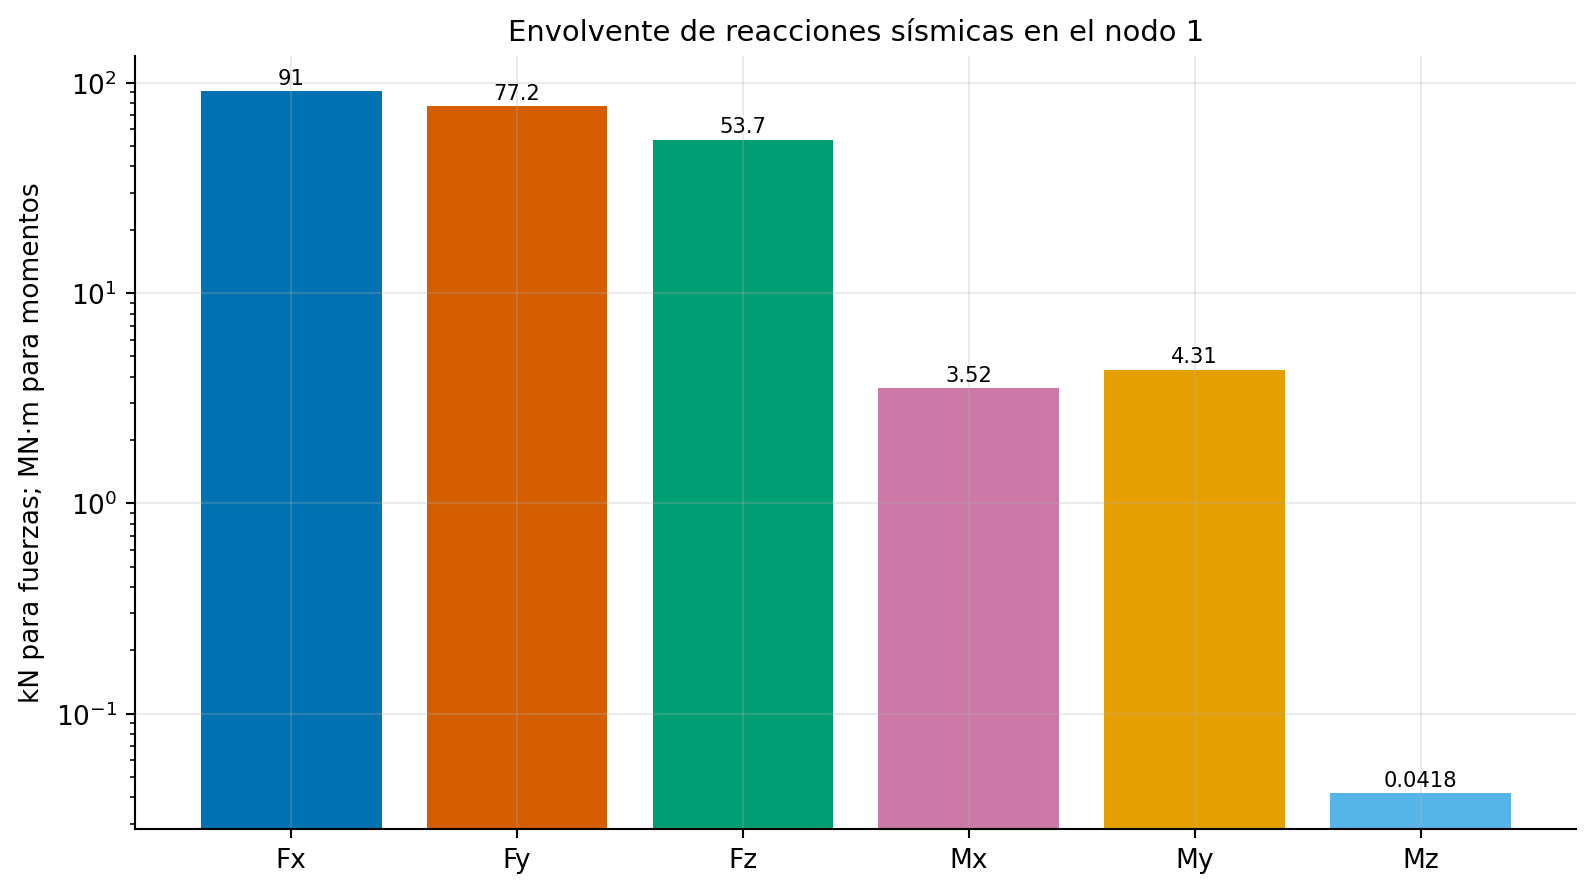
\includegraphics[width=\textwidth,height=0.69\textheight,keepaspectratio]{27_reacciones_base.png}
\caption{Reacciones máximas de base del caso rotante a 12 RPM; escala logarítmica común para las tres fuerzas y los tres momentos.}
\label{fig:resultado-origen-27}
\end{figure}

Se recuperaron fuerzas de extremo locales y globales para los 133 elementos. En el caso de 12 RPM, los máximos fueron: axial 71.706 kN en la pala, elemento 87; cortantes $V_2=75.892$ kN y $V_3=87.317$ kN en la torre, elemento 1; torsión 92.146 kN\,$\cdot$\,m en la transición, elemento 126; y momentos $M_2=3.992$ MN\,$\cdot$\,m y $M_3=3.394$ MN\,$\cdot$\,m en la torre, elemento 1.

\begin{figure}[!htbp]
\centering
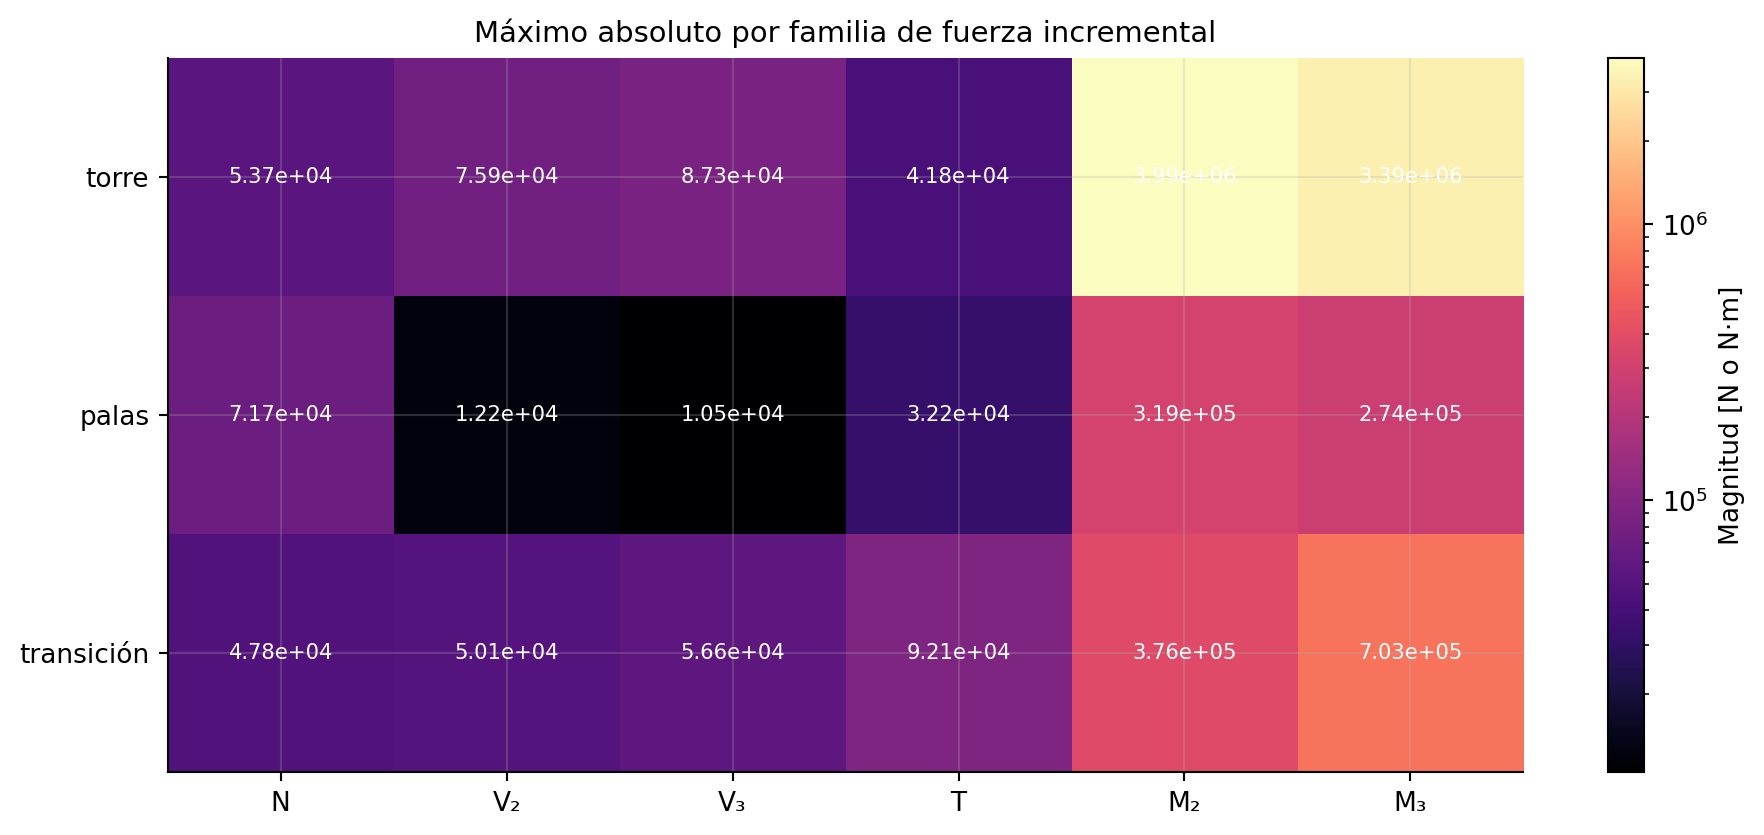
\includegraphics[width=\textwidth,height=0.69\textheight,keepaspectratio]{28_envolventes_fuerzas_elementales.png}
\caption{Envolventes del caso rotante a 12 RPM: axial, cortantes, torsión y momentos por familia de elemento. Son incrementos linealizados y no incluyen de nuevo la precarga estática.}
\label{fig:resultado-origen-28}
\end{figure}

\section{Qué puede concluirse y qué no}

\subsection{Conclusiones demostradas}

\begin{enumerate}
\item La conversión produce una turbina de 138 nodos y 133 elementos flexibles: 19 de torre, 105 de palas y 9 transiciones. Las MPC y el apoyo reducen $828\rightarrow810\rightarrow804$ GDL sin introducir resortes de penalización.
\item El elemento Timoshenko de 12 GDL tiene rango de rigidez 6 y nulidad 6. Sus seis primeros valores corresponden a tres traslaciones y tres rotaciones de cuerpo rígido; los seis restantes son modos deformacionales con frecuencias positivas entre 248.467 y 1010.603 Hz para el caso primitivo.
\item El modelo completo conectado conserva exactamente seis modos rígidos cuando está libre y ninguno cuando se fija la base. Por tanto, la primera frecuencia flexible no está contaminada por mecanismos espurios.
\item En la viga uniforme con 64 elementos, los errores relativos de desplazamiento, primera frecuencia y segunda frecuencia son $6.103\times10^{-5}$, $3.643\times10^{-5}$ y $5.838\times10^{-4}$, respectivamente, todos menores que $10^{-3}$.
\item La masa total es 2,601,611.15 kg. La masa consistente es la referencia; HRZ cambia hasta 1.0738\% las primeras ocho frecuencias de torre, lo que muestra que la distribución de masa, no solo su suma, afecta el espectro.
\item Entre 0 y 12 RPM, el desplazamiento máximo de equilibrio aumenta de 1.3915 a 1.4624 m y la norma centrífuga de 0 a 2.1867 MN. La carga centrífuga escala con $\Omega^2$ y las palas incrementan su tracción.
\item La giroscopía está dominada por el cubo y crece linealmente con la velocidad. El amortiguamiento Rayleigh de 1\% en 0.2 y 2 Hz es un supuesto, y las cargas aerodinámicas son nulas por ausencia de coeficientes de viento.
\item El QEP transforma 804 GDL en un lápiz de orden 1608. Las 12 ramas cubren 0.161234--1.599818 Hz a 0 RPM y cambian con el giro; aparecen coincidencias con 1P y 3P que deben tratarse como candidatos de resonancia.
\item Newmark reproduce el orden temporal dos. En el canal nodo 128--$u_y$, el máximo baja de 15.167 a 12.849 mm al pasar de 0 a 12 RPM; en el caso rotante se obtienen además reacciones y fuerzas internas incrementales.
\item No existe todavía un resultado de carga de viento: giro prescrito no equivale a excitación aerodinámica. Tampoco existe un criterio de capacidad que permita afirmar cumplimiento estructural o sísmico.
\end{enumerate}

\subsection{Límites que impiden una afirmación predictiva}

\begin{enumerate}
\item La rigidez y el amortiguamiento del tren 129--130 son parámetros de referencia, no datos calibrados.
\item Los CG de góndola y cubo están colocalizados con sus maestros porque no hay offsets medidos.
\item Las nueve transiciones tipo 4 son una herencia conservada, no una caracterización identificada del tren.
\item Los objetivos de Rayleigh no provienen de identificación modal experimental.
\item $\bm K_a=\bm C_a=\bm0$; la interfaz de tangentes no sustituye coeficientes físicos ni un análisis aeroelástico.
\item El registro sísmico es sintético: no hay espectro objetivo, escalamiento normativo, combinación direccional ni criterios de diseño.
\item El Campbell usa azimut congelado y espectro parcial; no es Floquet ni una certificación de estabilidad completa.
\item La cimentación flexible disponible es demostrativa y no fue calibrada.
\item La convergencia espacial se demostró en una viga analítica; falta refinar la turbina completa con una política físicamente defendible de interpolación de propiedades.
\item No existe todavía correlación con identificación modal, SCADA, mediciones de campo o un modelo de mayor fidelidad.
\end{enumerate}

\subsection{Trabajo científico recomendado}

La siguiente etapa científica es cerrar la identificación física:

\begin{enumerate}
\item obtener rigidez/amortiguamiento del tren y offsets/inercia completos;
\item calibrar modos y amortiguamiento contra medición o un modelo de referencia;
\item incorporar aerodinámica linealizada o aeroelástica con datos trazables;
\item seleccionar y escalar registros sísmicos según la norma aplicable;
\item modelar y calibrar suelo--cimentación;
\item ejecutar refinamiento de la turbina completa y análisis de sensibilidad e incertidumbre;
\item ampliar Campbell a periodicidad completa/Floquet cuando sea necesario;
\item comparar respuestas con mediciones o simulaciones independientes.
\end{enumerate}

\FloatBarrier
\bibliography{MECOM_2026_Useche}
\end{document}
